

%!TEX TS-program = latex
\documentclass[caractereUtf,maitrise]{style/scienceUdeS}

\long\def\beginpgfgraphicnamed#1#2\endpgfgraphicnamed{\includegraphics{#1}}


\usepackage{array}
% Pour inclure des sch\'emas en format pdf avec la commande
% \beginpgfgraphicnamed{figure_0}
% \endpgfgraphicnamed
% Voir pgfmanual \'a la page 654 pour plus d'information

% \usepackage{program}
\usepackage{algorithmic}
\usepackage{algorithm}
\usepackage[pdftex]{color}




%% Gabarit pour maitrise et pour maitrise GL
%%
%% Version 2010/08/11 v1.8
%%
%% Benoit Fraikin
%% Faculte des Sciences
%% Universite de Sherbrooke
%% Sherbrooke (Quebec), Canada

% =========================================== Options principales
% - bibliothequeNationale : pr\'esente le document pour la copie de la 
%   biblioth\`eque nationale. Attention, certaines commandes ne
%   fonctionnent plus.
%
% - caractereUtf : active les caract\`eres cod\'es en UTF8 au lieu du latin1
% - caractereLatin : active les caract\`eres cod\'es en latin1 au lieu du UTF8
%
% - logopdflatex : utilise le logo de l'universit\'e en pdf, pour ceux 
%   qui utilise pdflatex et non latex.
%
% - pasDeFigure : le document ne contient pas de figure (\begin{figure})
% - pasDeTableau : le document ne contient pas de tableau (\begin{table})
% - pasDeListing : le document ne contient pas de listing (\begin{lstlisting})
%
% - maitrise : pour une ma\^itrise en informatique
% - maitriseGL : pour une ma\^itrise en g\'enie logiciel
%                (ne diff\`ere pas de l'option "maitrise" pour l'instant)
% - these : pour une these de doctorat
% =========================================== Options secondaires
% - hypertexte
% - rectoverso
% - simpleface
% - draft
% - final
%=================================================================
% \newcommand{\co}{\color{blue}}

\newcommand{\co}{}


\begin{document}
%====================== DEBUT DU DOCUMENT ========================
\modeFrancais
% \include{contenu_maitrise/debut}

\newtheorem{frtheoreme}{Th\'eor\`eme}[section]
\newtheorem{frlemme}[frtheoreme]{Lemme}
\newtheorem{frprop}[frtheoreme]{Proposition}
\newtheorem{frcoro}[frtheoreme]{Corollaire}
\newtheorem{frdefinition}{D\'efinition}[section]


\auteur{Romain Cotte}
\titre{L'enjeu de la diff\'erentiation automatique dans les m\'ethodes de Newton d'ordres sup\'erieurs}


\MotsCles{diff\'erentiation automatique; Tapenade; optimisation; m\'ethode de Newton; ordres sup\'erieurs.}

% DESCRIPTION DU SOMMAIRE (EN FRANCAIS) -----------
\sommaire{
Les m\'ethodes plus avanc\'ees d'optimisation avec ou sans contraintes n\'ecessitent le calcul des d\'eriv\'ees
de la fonction. En ce sens, la diff\'erentiation automatique est devenu un outil primordial.
 Malgr\'e le fait qu'il soit omnipr\'esent, cet outil est encore en d\'eveloppement et en recherche. Il ne pr\'esente
pas les inconv\'enients classiques des m\'ethodes habituelles de d\'erivation mais reste complexe 
\`a utiliser. Ce travail consiste \`a utiliser un outil de diff\'erentiation permettant de calculer des d\'eriv\'ees 
d'ordres sup\'erieurs afin d'obtenir des directions am\'elior\'ees.
Nous d\'efinirons d'abord de mani\`ere g\'en\'erale un type d'algorithme d'optimisation \`a l'aide des directions suffisamment
 descendantes. Leurs caract\'eristiques seront analys\'ees pour modifier des m\'ethodes de type Newton afin d'avoir une
 meilleure fiabilit\'e de convergence. Nous \'etudierons les op\'erations critiques et l'ordre du coût de ces m\'ethodes\\
Dans une deuxi\`eme partie, nous verrons les calculs d'alg\`ebre lin\'eaire requis pour nos algorithmes
Ensuite, nous pr\'esenterons le fonctionnement de la diff\'erentiation automatique et en quoi c'en est un outil indispensable
 \`a ce genre de m\'ethodes.
Puis, nous expliquerons pourquoi nous avons choisi l'outil Tapenade pour la diff\'erentiation automatique et
 la librairie de Mor\'e, Garbow, Hillstrom pour la collection de fonctions tests.
Enfin, nous comparerons les m\'ethodes de types Newton.
}

% REMERCIEMENTS -----------------------------------
\remerciements{Je souhaite exprimer mes sinc\`eres remerciements \`a mon directeur de recherche, Jean-Pierre Dussault, qui 
a toujours \'et\'e disponible pour moi. Son aide m'a \'et\'e particuli\`erement pr\'ecieuse et m'a fait progresser pour aller de l'avant. C'est 
aussi une personne avec un cot\'e humain tr\`es agr\'eable et avec qui il a \'et\'e tr\`es int\'eressant et plaisant de travailler. \\
Ensuite, je voudrais remercier mes deux colocataires, Emmanuelle Meunier et Maggie Poudrier, qui furent tr\`es accueillantes et
chaleureuses. Elles m'ont fait d\'ecouvrir la r\'egion du Qu\'ebec et sont \`a l'image de ce que sont beaucoup de gens ici. \\
Je voudrais surtout remercier mes parents qui m'ont toujours soutenu dans mes \'etudes et qui me soutiendraient dans n'importe quel voie.
Enfin, je remercie Martin Guay, pour ses conseils et son soutient.
}

% LISTE DES ABREVIATIONS --------------------------
\abreviations{
  \begin{description}
  \item[AMPL] {\it A Mathematical Programming Language}
  \item[BK] {\it Bunch-Kaufman}
  \item[CUTEr] {\it A Constrained and Unconstrained Testing Environment, revisited}
  \item[DA] Diff\'erentiation Automatique
  \item[DED] Demi Espace de Diminution
  \item[GAO] Graphe Acyclique Orient\'e
  \item[INRIA] Institut National de Recherche en Informatique et en Automatique
  \item[LAPACK] {\it Linear Algebra PACKage}
  \item[MGH] {\it Mor\'e, Garbow et Hilstrom}
  \item[NaN] {\it Not a Number}
  \item[RA] {\it Recompute-All} Tout recalculer
  \item[SA] {\it Store-All} Tout stocker
  \item[SIF] {\it Standard Input Format}
  \end{description}
  \begin{description}
  \item[.]$M$ caract\`ere en majuscule pour les matrices
  \item[.]$c$ en minuscule pour les vecteurs colonnes
%$c=\left( \begin{array}{c}c_1\\c_2\\ \vdots  \\c_n\end{array}\right) $\\
  \item[.]$c^T$ la transpos\'ee : $c^T= \left( \begin{array}{cccc}c_1 & c_2 & \hdots  & c_n\end{array}\right) $
  \item[.]$\nabla f(x)$ le gradient de $f$ en $x$ : $\nabla f(x):\mathbb{R}^n\rightarrow \mathbb{R}$ une matrice ligne\\
$\nabla f(x)=
\left( \begin{array}{cccc} \frac{\partial f}{\partial x_1}& \frac{\partial f}{\partial x_2} 
 & \hdots  &\frac{\partial f}{\partial x_n}\end{array}\right)$ \\
$F(x)^T:=\nabla f(x) $

  \item[.]$\nabla^2 f(x)$ $: \mathbb{R}^n\rightarrow \mathbb{R}^n$ le hessien de la fonction.\\
$\nabla^2 f(x)= \left( \begin{array}{ccc}
 \frac{\partial^2 f}{\partial x_1\partial x_1} & \hdots & \frac{\partial^2 f}{\partial x_1\partial x_n}\\
 \vdots &  & \vdots \\
  \frac{\partial^2 f}{\partial x_n\partial x_1} & \hdots & \frac{\partial^2 f}{\partial x_n\partial x_1}
\end{array}
\right)$ sym\'etrique
 \item[.]$\#(f)$ correspond au coût de l'\'evaluation de $f$
 \item[.]{\tt [ ]} correspond \`a la liste vide
 \item[.]{\tt [$a$]} la liste compos\'ee d'un \'el\'ement : $a$
 \item[.]$::$ op\'erateur de contructeur de liste {\tt $a::$[ ]$=$[$a$], $t::\bar{q}$} o\`u $t$ est un \'el\'ement et $\bar{q}$ est une liste
 \item[.]$\lVert v\rVert=\lVert v\rVert_{2}=\sqrt{\sum_{i=1}^{n}v_i^2}=\sqrt{v^Tv}$
 \item[.]{\tt >\$} correspond au prompt bash sous unix
 \item[.] \verb!--->! correspond \`a {\it Scilab}
 \item[.] $\neg$ non logique
 

  \end{description}
}

%=================================================================
\modeFrancais{}
\enteteDeLaThese{}
\renewcommand{\chaptermark}[1]{\markboth{\textsc{\chaptername\ \thechapter.\ #1}}{}}
\renewcommand{\sectionmark}[1]{\markright{\textsc{\thesection. #1}}	}
    
%========================== INTRODUCTION ===========================

\modeFrancais{}
% \include{contenu_maitrise/introduction}
\Introduction


C'est par une repr\'esentation math\'ematique d'un ph\'enom\`ene physique, \'economique, humain que la programmation math\'ematique cherche \`a trouver
un optimum, c'est-\`a-dire l'\'etat jug\'e le meilleur ou le plus favorable \`a un probl\`eme. Plus pr\'ecis\'ement, la programmation non-lin\'eaire
est une m\'ethode permettant de r\'esoudre des \'equations et in\'equations qui g\'en\'eralement mod\'elisent le ph\'enom\`ene de notre mod\`ele.
Le but est de calculer un point minimisant (ou maximisant) une fonction objectif. Le probl\`eme peut être soumis \`a un ensemble de contraintes,
ce qui aura pour effet de r\'eduire le domaine de r\'ealisabilit\'e.
L'\'etude faite dans ce texte se limite \`a la programmation non-lin\'eaire sans contraintes. 
{\co 
Nous allons voir qu'il existe de nouveaux types d'algorithmes bas\'es sur celui de Newton. Ils b\'en\'eficient d'un meilleur ordre de convergence,
n\'eanmoins les calculs requis pour chaque it\'eration sont plus pouss\'es; calculs de d\'eriv\'ees d'ordre sup\'erieur.
 Ce travail consiste \`a utiliser les progr\`es de la Diff\'erentiation Automatique (DA) afin d'observer si le compromis entre l'ordre de convergence
et le temps de calcul est raisonnable.
 Le calcul de d\'eriv\'ees est un domaine complexe, d'autant plus que nous avons besoin d'efficacit\'e et de pr\'ecision d'une part et de pouvoir automatiser
ces calculs d'autre part.
Ainsi, l'outil de DA semble un outil id\'eal car contrairement aux diff\'erences finies, il est capable de fournir
le gradient de notre fonction \`a un coût proportionnel \`a l'\'evaluation de la fonction donc \`a un coût raisonnable. Par exemple, en grande dimension,
 de l'ordre de $10000$, alors qu'il faut plusieurs secondes pour obtenir le gradient par diff\'erences finies, la DA est capable de le calculer
 presque instantan\'ement ($\leq 4ms$). Bien qu'il soit encore en constant progr\`es, il a d\'ej\`a fait ses preuves
et est largement utilis\'e en optimisation comme avec le langage AMPL {\it A Mathematical Programming Language}.  
Un outil de DA a \'et\'e \'elabor\'e ({\it Sciad}) par Benoit Hamelin, et une estimation des coûts de calcul a \'et\'e faite 
par d\'ecompte du nombre d'op\'erations. Cependant, il n'est pas exploitable pour des grandes dimensions ($\geq 5$).
Nous allons d\'evelopper un environnement d'exp\'erimenation efficace au sein de {\it Scilab} afin de comparer les m\'ethodes d'optimisation
grâce \`a la DA qui concr\'etise les progr\`es pr\'ec\'edents en termes de temps de calcul.
Cet outil nous permettra d'atteindre des d\'eriv\'ees sup\'erieures. Cela ouvre la voie \`a de nouvelles m\'ethodes que nous 
allons tester. 

Dans une premi\`ere partie nous introduirons le probl\`eme d'optimisation, les m\'ethodes de descentes et leur complexit\'e parall\`element \`a leur ordre de convergence.
Ensuite, nous \'etudierons les op\'erations critiques; la r\'esolution de syst\`emes lin\'eaire d'une part et le calcul des d\'eriv\'ees d'autre part. Par cons\'equent, 
nous pr\'esenterons le fonctionnement de la DA avec deux modes d'ex\'ecution, le mode direct et le mode inverse qui ont diff\'erentes complexit\'es. Puis,
apr\`es avoir d\'etaill\'e les outils avec les r\'esultats obtenus nous comparerons les m\'ethodes d'ordres sup\'erieurs en terme d'it\'erations et de temps de calculs.

}


% Un article par chapitre
%=========================== CHAPITRE 1 ============================
\modeFrancais{}
\chapter[Algorithmes pour l'optimisation sans contraintes] 
        {\singlespacing%
         Algorithmes pour l'optimisation sans contraintes}
         \label{ch:chapitre-1}








\section{Introduction aux directions de descente}
Commençons par d\'efinir le contexte avec un peu de vocabulaire et les hypoth\`eses faites sur le probl\`eme. Puis nous allons analyser
 les concepts n\'ecessaires pour la suite. 
\subsection{Hypoth\`eses de travail}
Dans l'ensemble du texte, nous faisons deux hypoth\`eses : la continuit\'e, voir les d\'efinitions \ref{annexe:A:def}, et la diff\'erentiabilit\'e.
Soit le probl\`eme d'optimisation suivant :
\begin{equation}
\min_{x\in \mathbb{R}^n} f(x).
\label{eq:princ}
\end{equation}
Il s'agit d'un probl\`eme sans contraintes. La fonction objectif $f$, \`a valeurs de
 $\mathbb{R}^n$ dans $\mathbb{R}$, est continue et diff\'erentiable. L'ordre de diff\'erentiabilit\'e va d\'ependre de la m\'ethode choisie. 
 Cela exclut les probl\`emes en nombres entiers. On parle de probl\`eme d'optimisation \`a $n$ variables de d\'ecision avec $0<n$. 
Il existe deux types de solutions : les minima locaux, dont aucun point de leur voisinage n'est meilleur et les minima globaux, dont aucun des points
du domaine n'est meilleur. Par la suite, nous ne traiterons que les minima locaux. 

En notant $\nabla f(x) $ ou $F(x)^T:\mathbb{R}^n\rightarrow \mathbb{R}^n$ le gradient de la fonction objectif, une matrice ligne et 
$ \nabla^2f(x)$ ou $\nabla F(x): \mathbb{R}^n\rightarrow \mathbb{R}^{n\times n} $ son hessien, la condition n\'ecessaire d'optimalit\'e 
indique que si $x^*$ est un minimum local et que $f$ est diff\'erentiable dans un voisinage ouvert $V$ de $x^*$ alors 
\begin{equation}
\label{equ:prem}
\nabla f(x^*)=0.
\end{equation}
Ces points sont nomm\'es points stationnaires.
Si, de plus, $f$ est deux fois diff\'erentiable sur $V$ alors 
\begin{equation}
\label{equ:sec}
\nabla^2 f(x^*) \text{ est semi d\'efinie positive.}
% \label{eq:cond}
\end{equation}
La condition \eqref{equ:prem} s'appelle la condition n\'ecessaire du premier ordre et la condition \eqref{equ:sec} correspond \`a la condition n\'ecessaire du second ordre.
Lorsque la matrice est d\'efinie positive, il s'agit d'une condition suffisante, \cite{opt}.


\subsection{M\'ethodes avec recherche lin\'eaire}
Soit une fonction $f:\ \mathbb{R}^n \rightarrow \mathbb{R}$ continûment diff\'erentiable sur $\mathbb{R}^n$. {\co D\'efinissons
la fonction $h_{x,d}(\theta)=f(x+\theta d)$ qui permet de se placer dans le sous espace de $\mathbb{R}^n$ de dimension un.}
Pour le probl\`eme de minimisation \eqref{eq:princ}, les algorithmes couramment utilis\'es sont g\'en\'eralement les algorithmes de 
descente car ils permettent d'obtenir une convergence plus forte que pour des probl\`emes d'\'equations
non lin\'eaires.





 Donnons la d\'efinition d'une direction de descente.

%-----------------------D\'efinition direction de descente
\begin{frdefinition}
\label{def:1}
Soit $x \in \mathbb{R}^n$ et $d \neq 0$ un vecteur de $\mathbb{R}^n$, alors d est une direction de
descente de $f$ au point $x$ s'il existe $0<\theta_m$ tel que pour tout $\theta \in ]0,\theta_m]$,
$h_{x,d}(\theta)<f(x)$. \\
\end{frdefinition}
%
Il s'agit d'algorithmes it\'eratifs bas\'es sur le fait que si un point $x$ ne satisfait pas aux conditions d'optimalit\'e, alors il est 
possible de construire un autre point $x'$ qui v\'erifie $f(x')<f(x)$.
L'ensemble du {\it Demi Espace de Diminution} en $x$, not\'e $DED(x)$ est l'ensemble des directions qui satisfait \`a la relation :
$\nabla f(x)d<0$. Ces algorithmes ont tous la même forme;  trouver une direction dans le $DED(x)$ et 
ensuite approcher la fonction $h_{x,d}$ pour passer du point $x_k$ au suivant $x_{k+1}=x_k+\theta d$. N\'eanmoins, il faut s'assurer que la suite ${x_k}$
poss\`ede bien des points d'accumulation satisfaisant aux conditions.


%-----------------------D\'efinition direction suffisamment descente
\begin{frdefinition}
\label{def:2}
 Une direction d est consid\'er\'ee suffisamment descendante s'il existe deux constantes positives $\gamma_0$ et $\gamma_1$ 
 ind\'ependantes de $x$ telles que d satisfasse aux in\'egalit\'es suivantes : 

\begin{equation}  % L'environnement equation num\'erote
		  % l'\'equation. L'\'etoile sp\'ecifie de ne pas mettre
		  % de num\'ero
\label{equ:1}
\nabla f(x)d \leq -\gamma_0 \lVert \nabla f(x) \rVert^2 ,
\end{equation}
\begin{equation}
\label{equ:2}
\lVert d \rVert \leq \gamma_1 \lVert \nabla f(x) \rVert.
\end{equation}

%$$\nabla f(x)d \leq -\gamma_0 \lVert \nabla f(x) \rVert^2$$
%$$\lVert d \rVert \leq \gamma_1 \lVert \nabla f(x) \rVert$$
\end{frdefinition}






%Voici l'\'equation~\eqref{equ:1} qui est tr\`es p\'enible :




\begin{figure}
\caption{Directions suffisamment descendantes}
\begin{center}
  \beginpgfgraphicnamed{figures/figure_2}
  \endpgfgraphicnamed
\end{center}
\end{figure}
\noindent
Cette d\'efinition assure que toute direction $d$ utilis\'ee par un algorithme de descente est un vecteur assez long, et fait un angle assez
aigu avec l'oppos\'e de $\nabla f$. La strat\'egie, appel\'ee {\it linesearch}, consiste \`a minimiser $h_{x,d}(\theta)$ par rapport \`a $\theta$. %\min_{\theta}
\'Evidemment, le minimum $\theta_m$ est approximatif, nous aurons pas besoin d'une pr\'ecision aussi grande que le minimum $x^*$. 
On peut d\'emontrer que pour une point dans le voisinage de la solution v\'erifiant les conditions suffisantes du 
second ordre, pour des directions \'etudi\'ees dans ce m\'emoire, la recherche lin\'eaire n'est plus active.






\begin{frdefinition}
\label{def:3}
Un pas $\theta$ est dit admissible pour une direction suffisamment descendante $d$ lorsqu'il satisfait aux deux in\'egalit\'es suivantes, nomm\'ees
 crit\`ere d'Armijo et de Wolfe respectivement :
\begin{equation}
\label{equ:3}
f(x+\theta d)-f(x) \leq \tau_0 \theta \nabla f(x)d, \ \tau_0 \in ]0,\frac{1}{2}[
\tag{Armijo}
\end{equation}
\begin{equation}
\label{equ:4}
\tau_1 \nabla f(x)d \leq  \nabla f(x+\theta d)d , \ \tau_1 \in ]\tau_0,1[.
\tag{Wolfe}
\end{equation}
 


\end{frdefinition}

\paragraph{Famille de directions suffisamment descendantes}
Consid\'erons le cas g\'en\'eral d'une direction $\bar{d}=-H\nabla f(x)^T$, comme la direction de Newton, il s'agit d'une
transformation lin\'eaire de la direction de pente la plus forte. En supposant que $H$ est 
une matrice d\'efinie positive, alors la direction $\bar{d}$ v\'erifie les conditions d'une direction suffisamment 
descendante. En effet
$$\nabla f(x)\bar{d}=-\nabla f(x)H\nabla f(x)^T.$$
En notant $\lambda_{min}$ la plus petite valeur propre de H \ref{annexe:A:def} , on a
$$\nabla f(x)H\nabla f(x)^T \geq \lambda_{min} \lVert \nabla f(x)\rVert^2,$$
$$\nabla f(x)\bar{d}\leq -\lambda_{min}\lVert \nabla f(x)\rVert^2.$$
Et d'autre part $$\lVert \bar{d}\rVert \leq \lambda_{max}\lVert \nabla f(x)\rVert.$$
L'ensemble des algorithmes de descente peut être g\'en\'eralis\'e sous la forme suivante : %\ref{alg:1}.
\begin{algorithm}                     % enter the algorithm environment
\caption{Algorithme de descente}          % give the algorithm a caption
\label{alg:1}                           % and a label for \ref{} commands later in the document
\begin{algorithmic}  
\WHILE{$\neg$ fini}
\STATE $d \leftarrow$  direction qui satisfait la d\'efinition \ref{def:2}
\STATE $\theta \leftarrow$  qui satisfait la d\'efinition \ref{def:3}, les crit\`eres d'Armijo et Wolfe
\STATE $x_{k+1} \leftarrow x_k+\theta d$
\ENDWHILE
\end{algorithmic}
\end{algorithm}


\begin{frtheoreme}
Soit un algorithme de descente appliqu\'e au probl\`eme :\\
$$\min_{x\in \mathbb{R}^n} f(x), \ f \in \mathcal{C}^1(\mathbb{R}^n)$$
supposons qu'\`a chaque it\'eration, la direction utilis\'ee $d_k$ est une direction suffisamment descendante,
 et pour laquellle le pas utilis\'e dans cette direction est un pas admissible ; alors, tous les points
d’accumulation de la suite $\{x_k\}$ engendr\'ee par l'algorithme sont des points stationnaires pour le
probl\`eme $\min f(x)$.
\end{frtheoreme}




\section{Recherche lin\'eaire}
% ----------------------------------------------------
Pour s'assurer que les m\'ethodes utilis\'ees convergent correctement, une possibilit\'e est d'utiliser une recherche lin\'eaire. En effet, celle-ci
va nous garantir que l'on ne s'\'eloigne pas trop du point courant. La direction de Newton par exemple peut fournir des directions 
de norme \'elev\'ee et du même coup la convergence n'est pas syst\'ematique. Ceci se remarque d'autant que la dimension est grande.
Il existe plusieurs techniques pour nous assurer que la valeur de la fonction objectif diminue bien au court des it\'erations
si on poss\`ede une direction de descente, comme la r\'egion de confiance \cite{nocedal99}.




\section{M\'ethode de Newton}

% But : R\'esolution d'\'equations non lin\'eaires
% algorithme efficace pour trouver des approximations d'un z\'ero d'une fonction
% Soit $f:\mathbb{R}^n\rightarrow \mathbb{R}$ et le probl\`eme de trouver une solution
% au syst\`eme de n \'equations avec n inconnues :
% $$f_i(x_1,\hdots,x_n)=0, \ 1\leq i\leq n$$
% o\`u les $f_1,\hdots, f_n$ sont les composantes de $F$.
% On suppose que $F$ est continûment diff\'erentiable sur un ouvert convexe, ici $\mathbb{R}^n$ et 
% qu'il existe $x^*$ tel que $F(x^*)=0$ et $F'(x^*)$ est non singuli\`ere.

La m\'ethode de Newton joue un rôle central dans la r\'esolution d'\'equations non lin\'eaires et ainsi dans l'optimisation 
non lin\'eaire. Elle permet de trouver les racines d'une fonction. Comme le montre la condition n\'ecessaire du premier ordre,
il faut trouver un point tel que $F(x)^T:=\nabla f(x)=0$.

 L'id\'ee est de simplifier notre \'equation, tr\`es souvent complexe, en une \'equation plus simple : une \'equation 
quadratique. Pour obtenir cette simplification nous utilisons la relation de Taylor.


% 
% \begin{frdefinition}\textbf {(Mod\`ele lin\'eaire d'une fonction)} \\
% Soit $f:\mathbb{R}^n\rightarrow \mathbb{R}$ une fonction diff\'erentiable. Le mod\`ele lin\'eaire de $f$ en 
% $x^*$ est une fonction $l_{x^*}:\mathbb{R}^n\rightarrow \mathbb{R}$ d\'efinie par 
% \begin{equation}
% l_{x^*}(x)=f(x^*)+\nabla f(x^*)(x-x^*)
% \end{equation}
% o\`u $\nabla f(x^*)$ est le gradient de $f$ en $x^*$. 
% \end{frdefinition}


\begin{frdefinition}\textbf {(Mod\`ele quadratique d'une fonction)} \\
Soit $f:\mathbb{R}^n\rightarrow \mathbb{R}$ une fonction deux fois diff\'erentiable. Le mod\`ele quadratique de $f$ en 
$\bar{x}$ est une fonction $q_{\bar{x}}:\mathbb{R}^n\rightarrow \mathbb{R}$ d\'efinie par 
$$q_{\bar{x}}(x)=f(\bar{x})+\nabla f(\bar{x})(x-\bar{x})+\frac{1}{2}(x-\bar{x})^T\nabla^2 f(\bar{x})(x-\bar{x})$$
o\`u $\nabla f(\bar{x})$ est le gradient de $f$ en $\bar{x}$ et $\nabla^2 f(\bar{x})$ est la matrice hessienne de
$f$ en $\bar{x}$. En posant $d=x-\bar{x}$, on obtient la formulation \'equivalente : 
\begin{equation*}
q_{\bar{x}}(d)=f(\bar{x})+\nabla f(\bar{x})d+\frac{1}{2}d^T\nabla^2 f(\bar{x})d.
\end{equation*}
\end{frdefinition}
Si nous minimisons le mod\`ele quadratique au lieu de la fonction :
\begin{equation*}
\min_{d\in \mathbb{R}^n} q_{\bar{x}}(d)=f(\bar{x})+\nabla f(\bar{x})d+\frac{1}{2}d^T\nabla^2f(x)d.
\end{equation*}
%
La condition suffisante d'optimalit\'e du premier ordre nous donne :
\begin{equation*}
\nabla q_{\bar{x}}(d)=\nabla f(\bar{x})+\nabla^2f(x)d=0.
\end{equation*}
%
L'\'equation $\nabla^2 f(\bar{x})d_N=-\nabla f(\bar{x})$ est appel\'ee \'equation de Newton et $d_N$ direction de Newton.
En supposant que la matrice $\nabla^2f(x)$ est d\'efinie positive et donc inversible, la 
solution revient \`a trouver le minimum du mod\`ele quadratique de la fonction en $x_k$, d'o\`u :
\begin{equation*}
x_{k+1}=\arg\min_{x\in\mathbb{R}^n} q_{x_k}(x)
\end{equation*}
La solution peut s'\'ecrire 
\begin{equation*}
x_{k+1}\leftarrow x_k\underbrace{-\nabla F(x_k)^{-1}F(x_k)}_{d_N}
\end{equation*}
\begin{equation*}
\text{o\`u } d_N=-\nabla^2f(x)^{-1}\nabla f(x)^T.
\end{equation*}
% Cette direction correspond \`a la direction de Newton et elle intervient dans la 
% r\'esolution de syst\`emes d'\'equations non lin\'eaires. En notant
%  $F : \mathbb{R}^n \rightarrow \mathbb{R}^n$ le gradient de $f$, on recherche ses z\'eros. 
% $$x_{k+1}\leftarrow x_k\underbrace{-\nabla F(x_k)^{-1}F(x_k)}_{d_N}$$
% Cela revient au même de consid\'erer la fonction $F:\mathbb{R}^n\rightarrow \mathbb{R}^n$; c'est comme s'il y avait
% $n$ syst\`emes et $\nabla F(\bar{x})$ correspond au hessien.
% 
% 
% 
% 
%
L'id\'eal est de commencer \`a partir d'une approximation de $x^*$, notre minimum local; nommons le $x_0$. 
On calcule d'abord le mod\`ele quadratique en $x_0$ pour obtenir son minimum $x_1$. 
Si les conditions d'optimalit\'e sont satisfaites alors l'algorithme s'arrête, sinon on recalcule l'approximation
quadratique en $x_1$.
% En posant $d=x-x^*$, si on veut satisfaire la condition n\'ecessaire du premier ordre il faut que : 
% \begin{equation}
% l_{x^*}(x+d_N)=F(x^*)+\nabla F(x^*)d=0
% \end{equation}

\begin{figure}
\caption{Deux it\'erations de la m\'ethode de Newton dans $\mathbb{R}$}
\begin{center}
\fbox{
\begin{minipage}[c]{0.4\textwidth}
\begin{center}
\beginpgfgraphicnamed{figures/figure_7}
\endpgfgraphicnamed
\end{center}
\end{minipage}
}
\end{center}
\label{fig:Newton}
\end{figure}
%
Dans le cas unidimensionnel, avec plusieurs exp\'erimentations, nous pouvons constater que 
la m\'ethode de Newton converge tr\`es vite lorsque
\begin{itemize}
\item la fonction n'est pas trop non lin\'eaire c'est-\`a-dire que les variations de la fonction ne sont pas trop grandes
pour une petite variation de $x$.
\item la d\'eriv\'ee de la fonction n'est pas trop proche de $0$.
\item le point initial $x_0$ n'est pas trop loin de la solution.
\end{itemize}
Si une de ces conditions n'est pas satisfaite, il se peut que l'algorithme diverge.





Fourier \cite{convnewton} a d\'emontr\'e la convergence quadratique locale dans le cas r\'eel mais 
le th\'eor\`eme de Kantorovich nous assure la convergence sous certaines conditions dans le 
voisinage de $x_0$. De plus, il donne une borne de l'erreur pour chaque it\'er\'e.

\begin{frtheoreme}(Kantorovich \cite{Kantorovich})
\label{th:Kantorovich}
Soit $x_0 \in D_0$ tel que $\nabla F(x_0)^{-1}$ existe et que \\
$$\lVert \nabla F(x_0)^{-1} \rVert \leq B$$
$$\lVert \nabla F(x_0)F(x_0) \rVert \leq \eta$$
$$ \lVert \nabla F(x_0)- \nabla F(y)\rVert \leq K\lVert x-y \rVert \text{ pour tout }x\text{ et }y\text{ dans }D_0 $$
avec $h=BK\eta \leq \frac{1}{2}$\\
Soit $\Omega_*=\left\{x\ |\ \lVert x-x_0 \rVert \leq t^*\right\}$ o\`u $t^*=\left(\frac{1-\sqrt{1-2h}}{h} \right)\eta$\\
Si $\Omega_* \subset D_0$ alors les it\'erations de Newton; $x_{k+1}=x_k-\nabla F(x_k)^{-1}F(x_k)$ sont bien
d\'efinies, restent dans $\Omega_*$ et convergent vers $x_*\in \Omega_*$ tel que $F(x^*)=0$. De plus,
$$\lVert x_*-x_k \rVert \leq \frac{\eta}{h}\left(\frac{(1-\sqrt{1-2h})^{2^k}}{2^k}\right)\ k=0,\ 1,\ 2,\ \cdots$$
\end{frtheoreme}


Un th\'eor\`eme de convergence pour une m\'ethode it\'erative est appel\'e un th\'eor\`eme de convergence 
locale lorsque l'on suppose l'existence d'une solution $x^*$ et le point initial $x_0$ est 
suffisamment proche de $x^*$. D'autre part, un th\'eor\`eme de convergence tel que \ref{th:Kantorovich},
qui ne suppose pas l'existence d'une solution mais suppose certaines conditions sur $x_0$ est
appel\'e une th\'eor\`eme de convergence semi-locale.\\

Sans appliquer les conditions des d\'efinitions \ref{def:2} et \ref{def:3}, l'algorithme de Newton
a une convergence locale et semi-locale. 



\subsection{Ordre de convergence}
Pour pouvoir comparer les algorithmes, nous d\'efinissons la vitesse de convergence qui 
est le t\'emoin th\'eorique de l'efficacit\'e de la m\'ethode.

\begin{frdefinition}
\label{def:convergence}
La vitesse de convergence de la suite $\{x_k\}$ vers le point $x_*$, telle que $\forall k,\ x_k \neq x^*$ s'exprime 
\`a l'aide des scalaires $p$ et $\gamma$ dans l'expression suivante:
$$\lim \sup_{k\rightarrow \infty}\frac{\lvert x_{k+1}-x^*\rvert}{\lvert x_k-x^* \rvert^p}=\gamma< \infty $$
L'ordre de convergence de la suite est donn\'e par la plus grande valeur que p puisse prendre pour que la limite 
ci-haut demeure finie. Lorsque p=1, $\gamma$ est nomm\'ee le taux de convergence.
\end{frdefinition}

Le cas o\`u $p=1$ est dite convergence lin\'eaire, le cas $p=2$, convergence quadratique, $p=3$ cubique, plus $p$
est \'elev\'ee et plus la m\'ethode sera efficace.

\begin{frtheoreme}
Soit $x^*$ une racine isol\'ee de la fonction $g$ telle que $g'(x^*)\neq 0$, avec la fonction $g'$ lipschitzienne (\ref{annexe:A:def}), 
 Alors, il existe un voisinage de $x^*$ tel que si la m\'ethode de Newton 
est initialis\'ee dans ce voisinage, elle produit une suite convergeant vers $x^*$ et la vitesse de convergence 
asymptotique est quadratique.
\end{frtheoreme}


La condition pour que $x_0$ soit proche de la solution se traduit par la convergence locale, c'est-\`a-dire que $x_0$ doit
être choisi dans un certain voisinage de la solution.
Le fait que la fonction ne soit pas trop non lin\'eaire correspond au caract\`ere lipschitzien 
de la fonction. Par exemple, l'algorithme de Newton aura beaucoup de mal \`a trouver le z\'ero de l'\'equation
$\frac{1}{x}-C$ o\`u $C$ est une constante positive, si l'on part d'un point $x_0$ proche de z\'ero.
 Enfin, le th\'eor\`eme de Kantorovich suppose que $F(x_0)^{-1}$ existe. Pour un 
ordinateur il faudrait que $\lVert F(x_0)^{-1}\rVert \geq \epsilon>0$ \`a cause des erreurs
d'arrondis et d'annulation.

La direction $d_N$ est suffisamment descendante si la matrice $\nabla^2 f(x)$ est d\'efinie positive. Dans le 
cas contraire, la suite $\{x_k\}_k$ peut diverger, c'est pour cela que cette matrice va être modifi\'ee pour 
devenir d\'efinie positive.

\subsection{It\'eration de Newton modifi\'ee}

Dans le but de satisfaire les conditions pour la m\'ethode de descente, il faut modifier la direction $d_N$.
 Sinon, la m\'ethode peut ne plus être globalement convergente. 
De la même mani\`ere, on consid\`ere l'approximation d'ordre deux pour trouver le minimum de $f$ sauf qu'au lieu
d'avoir la matrice hessienne, nous avons une modification : $B_k$
$$f(x_k+d)=f(x_k)+\nabla f(x_k)d+\frac{1}{2}d^TB_kd$$ 
o\`u $B_k\simeq \nabla^2f(x)$. On va chercher le probl\`eme d'optimisation par rapport \`a la direction $d$ :
$$\min_d\nabla f(x_k)d+\frac{1}{2}d^TB_kd.$$
En d\'erivant par rapport \`a $d$, la condition n\'ecessaire du premier ordre fournit la relation :
$$\nabla f(x_k)^T+B_kd=0$$
$$d=-B_k^{-1}\nabla f(x_k)^T.$$
Le hessien $\nabla^2f(x)$ va être transform\'e pour le rendre d\'efini positif. Il suffit par exemple de prendre :
$$B_k=\nabla^2 f(x_k)+\max(-\lambda_{min}+\epsilon,0)I$$
o\`u $\lambda_{min}$ est la plus petite valeur propre de $\nabla^2 f(x_k)$ et $\epsilon>0$.


L'inconv\'enient de cette formule est dans le calcul de $\lambda_{min}$, il faut avoir l'ensemble des valeurs propres (voir \ref{annexe:A:def})  de
la matrice et ce calcul a une complexit\'e en $\mathcal{O}(n^3)$ avec une constante implicite plutôt d\'efavorable. 
Nous allons directement nous aider de la d\'ecomposition de Cholesky pour modifier la diagonale. Ainsi, on esp\`ere avoir
une complexit\'e totale inf\'erieure.
% Pour cela, nous utiliserons une d\'ecomposition de Cholesky modifi\'ee pour que toutes les 
% valeurs propres soient strictement positives.

% Convergence locale quadratique




%   Voir \ref{chap3:cholesky}.


% \section{R\'egion de confiance}
% Une autre technique qui nous permet de ne pas trop s'\'ecarter du point courant est la m\'ethode par r\'egion de confiance. La zone de 
% confiance, de laquelle on ne va pas pouvoir s'\'ecarter va être d\'etermin\'ee par approximation quadratique de la fonction. Si cette
% approximation est trop erron\'ee, la zone devra être r\'eduite, sinon, nous l'augmenterons.\\



\section{M\'ethodes d'ordre sup\'erieur \`a deux}
Les m\'ethodes de Halley et de Chebychev sont des techniques c\'el\`ebres pour r\'esoudre des \'equations non lin\'eaires. Ces algorithmes
sont tr\`es proches de la m\'ethode de Newton et ont une convergence cubique. Le gain de convergence s'obtient par une analyse
plus pr\'ecise de la fonction puisqu'elles requi\`erent la d\'eriv\'ee seconde de $F$ donc la d\'eriv\'ee troisi\`eme de l'objectif $f$.
En fin de section nous verrons une m\'ethode du même type qui a fait l'objet de recherches r\'ecentes.

\subsection{M\'ethode de Halley}
Cette m\'ethode a \'et\'e d\'ecouverte par Edmond Halley (1656-1742), elle s'applique \`a une fonction $\mathcal{C}^2$.
Au lieu de faire une approximation lin\'eaire de la fonction $F$, on part d'une approximation quadratique :
$$F(x+d)=F(x)+\nabla F(x)d + \frac{1}{2}d^T\nabla^2F(x)d + \mathcal{O}({\lVert d\rVert^3}) $$
Cauchy a d\'emontr\'e sous certaines conditions la convergence semi-locale cubique.
En effectuant le d\'eveloppement de Taylor limit\'e $\sqrt{1-x}\simeq 1-\frac{1}{2}x $, on obtient la m\'ethode de Halley (1694):
$$x_{k+1}=x_k-[\nabla F(x_k)-\frac{1}{2}\nabla^2F(x_k)\nabla F(x_k)^{-1}F(x_k)]^{-1}F(x_k)$$
%
Cela revient \`a r\'esoudre les diff\'erents syst\`emes : 
$$F(x_k)+\nabla F(x_k)c_k=0 \Leftrightarrow c_k=-\nabla F(x_k)^{-1}F(x_k)$$
$$F(x_k)+\nabla F(x_k)d_k+\frac{1}{2}\nabla^2F(x_k)c_kd_k=0  \Leftrightarrow  d_k=-[\nabla F(x_k)-\frac{1}{2}\nabla^2F(x_k)c_k]^{-1}F(x_k)$$
$$x_{k+1}=x_k+d_k, 0\leq k$$



\subsection{M\'ethode de Chebychev}


Chebyshev proposa une m\'ethode d'ordre deux en 1841, de convergence cubique :
\begin{equation}
x_{k+1}=x_k-\nabla F(x_k)^{-1}F(x_k)-\frac{1}{2}\nabla F(x_k)^{-1}\nabla^2F(x_k)[\nabla F(x_k)^{-1}F(x_k)]^2
\label{equ:cheb}
\end{equation}
ce qui revient \`a r\'esoudre :
$$F(x_k)+\nabla F(x_k)c_k=0 \Leftrightarrow c_k=-\nabla F(x_k)^{-1}F(x_k)$$
$$F(x_k)+\nabla F(x_k)d_k+\frac{1}{2}\nabla^2F(x_k)c_k^2=0 \Leftrightarrow  d_k=-c_k-\frac{1}{2}\nabla F(x_k)^{-1}\nabla^2F(x_k)c_k^2$$
$$x_{k+1}=x_k+d_k, 0\leq k$$




\subsection{M\'ethode d'extrapolation d'ordre trois}

% En consid\'erant chacune de ces m\'ethodes comme des directions de d\'eplacement,
%  on g\'en\`ere de nouveaux algorithmes. Globalement, on peut r\'esumer ces m\'ethodes
%  comme suit:\\

Les m\'ethodes pr\'esent\'ees peuvent être r\'esum\'ees comme suit. Soit $F$ une fonction de $\mathbb{R}^n$
dans $\mathbb{R}^n$. Chaque m\'ethode est vue comme une direction de d\'eplacement avec laquelle une 
suite d'it\'er\'es est construit \[x_{k+1}=x_k+d_k\]
La condition n\'ecessaire du premier ordre doit être satisfaite, on cherche $x^*$ tel que 
\[F(x^*)=0\]
La m\'ethode de Newton revient \`a r\'esoudre le syst\`eme : 
\[F(x)+\nabla F(x)d_N=0.\]
Celle de Halley revient \`a faire : 
\[F(x)+\nabla F(x) d_H+\frac{1}{2} \nabla^2 F(x)d_N d_H=0.\]
Et celle de Chebychev :
\[F(x)+\nabla F(x) d_C+\frac{1}{2}\nabla^2 F(x)d_Nd_N=0.\]
%
%
% \red 
\`A partir de ces directions de Halley, Newton et Chebyshev, d'apr\`es \cite{Kchouk}, on peut d\'evelopper de nouvelles m\'ethodes sur le même plan
mais \`a un ordre sup\'erieur : 

\begin{equation}
 F(x)+\nabla F(x)d+\frac{1}{2}\nabla^2 F(x){
d_1d_2}+\frac{1}{6}\nabla^3 F(x){
 d_3d_4d_5}=0
\label{eq:extra}
\end{equation}
o\`u la direction recherch\'ee est $d$ et les directions $d_i$ sont des directions connues.


% Ces m\'ethodes peuvent être illustr\'ees par les dessins pr\'esent\'es ici. Ils repr\'esentent les zones de convergence (ou bassin d'attractions) de chaque m\'ethode, c'est-\`a-dire les surfaces \`a l'int\'erieur desquelles un point de d\'epart x0 va converger vers une solution donn\'ee en un nombre d\'etermin\'e d'it\'erations. On observe, d\'ependamment de la m\'ethode choisie, des surfaces plus ou moins grandes et plus ou moins homog\`enes. Ces bassins d'attractions r\'esument l'information sur les convergences des m\'ethodes.


% \section{M\'ethode de Super-Halley}
% $$x_{k+1}=x_k-[I+\frac{1}{2}L(x_k)(I-\alpha L(x_k)^{-1}]\nabla F(x_k)^{-1}F(x_k)$$
% o\`u $$L(x)=\nabla F(x){-1}\nabla^2 F(x)\nabla F(x)^{-1}F(x)$$





Les m\'ethodes qui viennent d'être pr\'esent\'ees ne sont pas universelles et souffrent des 
mêmes d\'efauts que la m\'ethode de Newton \`a savoir que la convergence est seulement locale et les fonctions
doivent être lipschitziennes. Comme la plupart des algorithmes en optimisation, il
n'existe pas de m\'ethode meilleure que toutes. Dans certains cas de figure, les m\'ethodes qui sont a priori
moins efficaces ; c'est-\`a-dire de moins bonne convergence, peuvent r\'esoudre certains programmes non lin\'eaires en moins d'it\'erations.


\section{Ordre de la complexit\'e}
\label{chap1:ordre}
Une borne th\'eorique de la complexit\'e bien connue est celle de Griewank \cite{Iri89onautomatic}, qui \'enonce que 
le coût d'\'evaluation du gradient n\'ecessite jamais plus de cinq fois le coût de l'\'evaluation
de la fonction en mode inverse et $n$ fois le coût de l'\'evaluation en mode direct.
Par ailleurs, Mihael Ulbrich et Stephan Ulbrich \cite{Ulbrich} donnent des bornes plus pr\'ecises sur les deux modes tangent et direct
de la DA, \'etudi\'es plus loin au chapitre \ref{sec:da}.
En notant $\#(f)$, le coût d'\'evaluation de $f$, les bornes de complexit\'e pour le mode direct sont :

$$(n+1)\#(f) \leq \#(f,\nabla f)\leq (3n+1)\#(f)$$
$$\frac{n^2+3n+2}{2}\#(f) \leq \#(f,\nabla f,\nabla^2f)\leq \frac{7n^2+11n+2}{2}\#(f)$$
%
On remarque qu'en mode direct, le coût du gradient est de l'ordre de la dimension de l'espace de d\'efinition par le coût de la fonction.
Cela va vite devenir lourd si nous voulons obtenir des ordres trois, voire quatre.
En revanche, avec le mode inverse la borne de complexit\'e, dûe \`a W. Baur et V. Strassen\cite{Baur}, ne d\'epend plus de $n$ et nous avons :
\begin{equation*}
\#(f,\nabla f)\leq 4\#(f)
% \tag{W. Baur et V. Strassen\cite{Baur}}
\end{equation*}
\begin{equation*}
\#(f,\nabla^2 f)\leq 16n\#(f)
\end{equation*}


En r\'ealit\'e, dans beaucoup de cas, nous avons besoin du calcul du gradient multipli\'e par un vecteur ou de la hessienne multipli\'ee par un vecteur, ce qui va simplifier la 
complexit\'e avec la DA.
Bien qu'il y ait une remarque sur l'op\'eration $\nabla^2 f.d $, M. et S. Ulbrich ne donnent pas de borne pr\'ecise pour cette op\'eration.
Quand on applique le mode direct dans une certaine direction, le coût est proportionnel au coût de $f$. En g\'en\'eralisant aux d\'erivations
sup\'erieures, les op\'erations $\nabla^3 f\cdot u \cdot v$ et $\nabla^4 f\cdot u \cdot v \cdot w$ ne d\'ependent pas de $n$. Ce qui est 
le plus surprenant dans le tableau c'est qu'il est possible d'obtenir le gradient qui est de dimension $n$ \`a un coût proportionnel \`a
la fonction. Intuitivement, on pourrait croire qu'il est possible d'obtenir de la même mani\`ere les hessiens et ordres plus \'elev\'es avec 
le même coût. En r\'ealit\'e, nous verrons que ce r\'esutlat ne peux pas s'obtenir avec une certaine contrainte de stockage.

\begin{center}
\begin{tabular}{|l|r|}\hline
Op\'eration  & coût \\\hline
Gradient : $\nabla f(x)$ & $\leq 4\#(f)$ \\
Hessien : $\nabla^2 f(x)$ & $\leq 16n\#(f)$ \\
Hessien$\times$ vecteur : $\nabla^2 f(x)\cdot v$ & $\mathcal{O}(\#(f))$\\
$\nabla^3 f\times$ vecteur $\times$ vecteur : $\nabla^3 f(x)\cdot v_1\cdot v_2$ & $\mathcal{O}(\#(f))$\\
$\nabla^3 f\times$ vecteur : $\nabla^3 f(x)\cdot v_1$ & $\mathcal{O}(n\#(f))$\\
$\nabla^4 f\times$ vecteur $\times$ vecteur$\times$ vecteur : $\nabla^4 f(x)\cdot v_1\cdot v_2\cdot v_3$ & $\mathcal{O}(\#(f))$\\
% D\'ecomposition de Cholesky : $A+E=LDL^T$ & $\mathcal{O}(n^3)$\\
% Changement de la diagonale : $\hat{D}\leftarrow D $ & $\mathcal{O}(n)$\\
% R\'esolution & $\mathcal{O}(n^2)$\\
\hline
\end{tabular}
\end{center}

\noindent
Bien sûr, il s'agit de bornes approximatives, nous verrons ce qu'il en est en pratique. Voyons maintenant en d\'etail
l'ordre de complexit\'e de chaque m\'ethode.
% Ceci est d'un point de
% verrons que les proc\'ed\'es de diff\'erentiation automatique pour des dimensions \'elev\'ees d\'ependent de la capacit\'e de stockage.

% Gradient : $\leq 5\times C(f)$\\
% Hessien : $n C(f)$ \\
% Hessien$\times$Vecteur : $n \times C(f)$\\
% Tenseur$\times$Vecteur : \\
% Tenseur$\times$Vecteur$\times$Vecteur : \\
% Factorisation pour inversion et r\'esolution : $\mathcal{O}(n^3)$\\
% Changement de la diagonale : $\mathcal{O}(n)$\\
% R\'esolution : $\mathcal{O}(n^2)$\\


\subsection{Newton modifi\'e}
Pour calculer la direction de Newton modifi\'ee, le calcul du gradient et du hessien sont
 n\'ecessaires. En effet, la direction est obtenue en r\'esolvant le syst\`eme
$$\nabla^2 f(x)d_N=-\nabla f(x)^T\leftrightarrow d_N=-\left[\nabla^2 f(x)\right]^{-1}\nabla f(x)^T$$
la matrice $\nabla^2 f(x)$ est carr\'ee et sym\'etrique puisque
 \begin{align*}
\left[\nabla^2 f(x)\right]_{ij} & =\frac{\partial^2 f(x)}{\partial x_i \partial x_j} \\
				& = \frac{\partial^2 f(x)}{\partial x_j \partial x_i} \\
				& = \left[\nabla^2 f(x)\right]_{ji} 
\end{align*}


\begin{algorithm}%[h]                     % enter the algorithm environment
\caption{Direction de Newton modifi\'ee}          % give the algorithm a caption
\label{alg:2}                           % and a label for \ref{} commands later in the document
\begin{algorithmic}  
\STATE \textbf{Pr\'ealables:} %Variables en entr\'ee :  
\begin{itemize}
\item[$\bullet$] $\nabla f(x)\in \mathbb{R}^n$ le gradient en $x$
\item[$\bullet$] $\nabla^2 f(x)\in \mathbb{R}^{n\times n}$ le hessien en $x$
\end{itemize}
\STATE \textbf{Variable en sortie:} $r$
% \hline
\STATE $g \leftarrow \nabla f(x)^T$
\STATE $H \leftarrow \nabla^2 f(x)$
\STATE $A,P \leftarrow $ d\'ecomposition de $H$
\COMMENT{$P$ \'etant la matrice de permutation}
\STATE $A' \leftarrow$ modification de la diagonale de $A$
\STATE $d_N \leftarrow$ r\'esolution($A',\ P,\ g)$ 
\COMMENT{R\'esolution du syst\`eme $A^{''}x=g$ o\`u $A^{''}$ est la matrice $A'$ avec les bonnes permutations}

%[R\'esolution du syst\`eme $A^{''}x=g$ o\`u $A^{''}$ est la matrice $A'$ avec les bonnes permutations]

\STATE $r\leftarrow (d_N,A',P)$ 
\COMMENT{On retourne la direction mais aussi la
 d\'ecomposition et la permutation que l'on pourra r\'eutiliser par la suite}
\end{algorithmic}
\end{algorithm}


% Le nombre d'addition requis pour cette d\'ecomposition est $\frac{1}{6}n^3+\frac{3}{2}n^2$ et  $\frac{1}{6}n^3+n^2$ 

% \begin{verbatim}
% function [d,g,h,ABmod,Ipiv]= Dn(x,n,m)
%     g=G(x,n,m);
%     h=H(x,n,m);
%     [ABmod , Ipiv] = mfact(h);
%     d=-msol(ABmod,Ipiv,g)
% endfunction
% \end{verbatim}

% \begin{frtheoreme}(Cauchy \cite{cauchy})
% Soit $X=\\mathbb{R}$, $F=f\in C^2$, $x_0 \in X$, $f'(x_0)\neq 0$, $\sigma_0=-f(x_0)/f'(x_0)$, $\eta=\lvert \sigma_0 \rvert$,\\
% $I=\left\{\begin{array}{rcl}
% [x_0,\ x_0+2\sigma_0] & \mbox{si} & \sigma_0 \geq 0 \\
% [x_0+2\sigma_0,\ x_0] & \mbox{si} & \sigma_0<0 \\
% \end{array}\right.$\\
% Et $\lvert f^{''}(x) \rvert \leq K$ dans $I$. Alors, on a le r\'esultat suivant :\\
% $(i)$ Si \\
% $2K\eta < \lvert f'(x_0)\rvert$,
% alors \ref{} a une unique solution $x^*$ dans $I$\\
% $(ii)$ Si $\lvert f'(x)\rvert \geq m$ dans $I$ et \\
% $2K\eta < m$,\\
% alors la s\'equence de Newton {$x_k$} commençant \`a $x_0$ satisfait :\\
% $\lvert x_{k+1} \rvert \leq \frac{K}{2m}\lvert x_k -x_{k-1} \rvert^2$, $k\geq 1$\\
% et \\
% $x^* \in [x_k, \ x_k+2\sigma_k] $, o\`u $\sigma_k =-f(x_k)/f'(x_k)=k_{k+1}-x_k$, et ainsi \\
% $\lvert x^*-x_k \lvert \leq 2\x_{k+1}-x_k\rvert$ ($k\geq 0$)\\
% $\leq \frac{K}{m}\lvert x_k-x_{k-1}\rvert^2 (k\geq 1)$ \\
% $\leq 2\eta\left( \frac{K\eta}{2m} \right)^{2k-1} (k\geq 0)$ 
% \end{frtheoreme}
\noindent
L'algorithme \ref{alg:2} r\'esume les \'etapes du calcul de la direction de Newton modifi\'ee.
La matrice $\nabla^2 f(x)$ est factoris\'ee pour pouvoir r\'eutiliser la d\'ecomposition. 
$P$ est un vecteur qui contient les informations sur les permutations \`a faire et la matrice $A$ est
modifi\'ee pour obtenir une direction de descente lorsque la matrice n'est pas d\'efinie positive (\ref{annexe:A:def}).
Pour chaque calcul de la direction en $x$ les op\'erations sont 
\begin{itemize}
\item Calcul du hessien $\nabla^2 f(x)$
\item Factorisation $LDL^T=PAP^T$
\item Changement de la diagonale $D'=D+\Tilde{D}$
\item R\'esolution de syst\`emes triangulaires $Lx=b$ 
\end{itemize}

Ce qui a un comportement en $\frac{n^3}{3}+n^2$ et la convergence est quadratique.


\subsection{Chebychev}

Pour calculer la direction de Chebychev $d_C$, on va r\'eutiliser le calcul 
de la direction de Newton qui apparaît plusieurs fois dans l'\'equation \eqref{equ:cheb}. %ligne 505

\begin{algorithm}                     % enter the algorithm environment
\caption{Direction de Chebychev}          % give the algorithm a caption
\label{alg:3}                           % and a label for \ref{} commands later in the document
\begin{algorithmic}  
\STATE \textbf{Pr\'ealables:} %Variables en entr\'ee :  
\begin{itemize}
\item[$\bullet$] $\nabla f(x)\in \mathbb{R}^n$ le gradient en $x$
\item[$\bullet$] $\nabla^2 f(x)\in \mathbb{R}^{n\times n}$ le hessien en $x$
\item[$\bullet$] La fonction $g\in \mathbb{R}^n\times\mathbb{R}^n \rightarrow \mathbb{R}^{n} : u,\ v \mapsto \nabla^3 f(x)\cdot u\cdot v$ qui fait le calcul en fonction
de deux vecteurs quelconques $u$ et $v$
\item[$\bullet$] $(d_N,A',P)\leftarrow$ Direction de Newton
\end{itemize}
% \STATE Variables en entr\'ee :  $g : v,\ y \mapsto \nabla^3 f(x).v.y$, $r \leftarrow$ Direction de Newton
% [$\mapsto$ indique qu'il s'agit d'une fonction, nous n'avons pas besoin de $\nabla^3 f(x)$ en entier]

\STATE \textbf{Variable en sortie :} $d_C$
\STATE $w \leftarrow \nabla^3 f(x) \cdot d_N \cdot d_N = g(d_N,d_N)$
\STATE $d \leftarrow$ r\'esolution($A',\ P,\ w)$ 
\STATE $d_C \leftarrow d_N-\frac{1}{2}d$
\end{algorithmic}
\end{algorithm}


 $w=\nabla^2 (\nabla f(x)\cdot d_n)\cdot d_n$ contient un tenseur $\times$ vecteur$\times$ vecteur donc un vecteur.\\
%  $A'$ contient la d\'ecomposition de A avec les \'el\'ements diagonaux modifi\'es.

Pour chaque calcul de la direction de Chebychev :
\begin{itemize}
\item Calcul de la direction de Newton : l'algorithme r\'eutilise les valeurs calcul\'ees dans l'algorithme de Newton.
\item $\nabla^3 f(x)\cdot d\cdot d$
\item R\'esolution de syst\`emes triangulaires $Lx=b$ 
\end{itemize}

La complexit\'e de la direction de Chebychev est de l'ordre de $\frac{n^3}{3}+(2+C)n^2$ et la m\'ethode a une convergence cubique.




\subsection{Halley}

Pour calculer la direction de Halley $d_H$, on va r\'eutiliser le calcul 
de la direction de Chebychev et de Newton. %Voir l'algorithme \ref{alg:4}

\begin{algorithm}                     % enter the algorithm environment
\caption{Direction de Halley}          % give the algorithm a caption
\label{alg:4}                           % and a label for \ref{} commands later in the document
\begin{algorithmic}  
\STATE \textbf{Pr\'ealables:} %Variables en entr\'ee :  
\begin{itemize}
\item[$\bullet$] $\nabla f(x)\in \mathbb{R}^n$ le gradient en $x$
\item[$\bullet$] $\nabla^2 f(x)\in \mathbb{R}^{n\times n}$ le hessien en $x$
\item[$\bullet$] La fonction $g\in \mathbb{R}^{n} \rightarrow \mathbb{R}^{n\times n} : u \mapsto \nabla^3 f(x)\cdot u$ qui effectue
 le produit scalaire du tenseur $\nabla^3 f(x)$ et d'un vecteur
\item[$\bullet$] $(d_N,A',P)\leftarrow$ Direction de Newton
\item[$\bullet$] $d_C\leftarrow$ Direction de Chebychev

\end{itemize}
% \STATE Variables en entr\'ee :  $g : v,\ y \mapsto \nabla^3 f(x).v.y$, $r \leftarrow$ Direction de Newton
% [$\mapsto$ indique qu'il s'agit d'une fonction, nous n'avons pas besoin de $\nabla^3 f(x)$ en entier]

\STATE \textbf{Variable en sortie :} $d_C$
\STATE $A \leftarrow \nabla^3 f(x) \cdot d_N$
\STATE $M \leftarrow \frac{1}{2}A+\nabla^2 f(x)$
\STATE $d_H \leftarrow$ r\'esolution($Md_H=\nabla f(x)^T)$ 
\end{algorithmic}
\end{algorithm}



\begin{itemize}
\item Calcul de la direction de Chebychev et donc celle de Newton
\item $\nabla^3 f(x)\cdot v$
\item D\'ecomposition de Cholesky modifi\'ee
\item Changement de la diagonale
\item R\'esolution de syst\`emes triangulaires $Lx=b$ 
\end{itemize}



Soit un coût de $\frac{2}{3}n^3+(2+C+D)n^2$ o\`u $C$ et $D$ sont des constantes d\'ependantes de l'efficacit\'e du logiciel de DA.
Pour rappel, cette m\'ethode a une convergence cubique.
Pour bien comprendre la difficult\'e, pour effectuer cette m\'ethode, il faut être capable de calculer $\nabla^3 f(x)\cdot d$ pour une 
certaine direction $d$.




\subsection{Extrapolation d'ordre trois}


\begin{algorithm}                     % enter the algorithm environment
\caption{Direction d'extrapolation d'odre trois}          % give the algorithm a caption
\label{alg:3}                           % and a label for \ref{} commands later in the document
\begin{algorithmic}  
\STATE \textbf{Pr\'ealables:} %Variables en entr\'ee :  
\begin{itemize}
\item[$\bullet$] $(d_N,A',P)\leftarrow$ Direction de Newton
\item[$\bullet$] $d_C \leftarrow$ Direction de Cheychev 
\item[$\bullet$] La fonction $g: u,\ v \mapsto \nabla^3 f(x)\cdot u\cdot v$ qui fait le calcul en fonction
de deux vecteurs quelconque $u$ et $v$
\item[$\bullet$] La fonction $h: u,\ v,\ w \mapsto \nabla^4 f(x)\cdot u\cdot v\cdot w$
\end{itemize}
\STATE \textbf{Variable en sortie :} $d_3$
\STATE $d \leftarrow 2d_C-d_N$
\STATE $v \leftarrow$ $\nabla^3 f(x).d.d_N$
\STATE $w\leftarrow$ r\'esolution($A',\ P,\ v)$ 
\STATE $z\leftarrow\nabla^4 f(x).d_N^3=h(d_N,d_N,d_N)$
\STATE $t\leftarrow$ r\'esolution($A',\ P,\ z)$ 
\STATE $d_3 \leftarrow d_N-\frac{1}{2}w-\frac{1}{6}t$
\end{algorithmic}
\end{algorithm}


Les op\'erations requises sont :

\begin{itemize}
\item Calcul de la direction de Chebychev et donc celle de Newton
\item $\nabla^3 f(x)\cdot d\cdot d$
\item $\nabla^4 f(x)\cdot d\cdot d\cdot d$
\item Deux r\'esolutions de syst\`emes triangulaires $Lx=b$ 
\end{itemize}

Le coût total est de l'ordre de $\frac{1}{3}n^3 +(3+C+E)n^2$ o\`u $C$ et $E$ vont d\'ependre de l'outil de DA et avec une convergence
quartique.



\subsection{R\'esum\'e}
R\'esumons l'ordre de convergence et la complexit\'e des calculs sous forme d'un tableau. Les r\'esolutions des syst\`emes lin\'eaires
et la modification de la diagonale sont n\'eglig\'es par rapport aux autres calculs.\\

\begin{tabular}{|l|c|c|c|}\hline
M\'ethode & Ordre du coût par rapport \`a $\#(f)$ & Convergence \\
\hline
Newton modifi\'e& $\frac{1}{3}n^3+n^2$ & quadratique\\
Chebychev & $\frac{1}{3}n^3+(2+C)n^2$  & cubique \\
Halley & $\frac{2}{3}n^3+(2+C+D)n^2$ & cubique \\
Extrapolation d'ordre 3 & $\frac{1}{3}n^3 +(2+C+E)n^2$  & quartique \\
\hline
\end{tabular}\\


\noindent
Ainsi, on peut observer que pour le même ordre de complexit\'e, la convergence de l'algorithme de 
Chebychev est meilleure que celle de Newton. Si nous arrivons \`a atteindre les bornes th\'eoriques des calculs, la m\'ethode 
de Chebychev devrait prendre moins de temps d'ex\'ecution surtout pour des dimensions plus \'elev\'ees pour att\'enuer la constante $C$.
De plus, il va être int\'eressant de comparer les m\'ethodes classiques avec l'extrapolation d'ordre trois puisqu'elle a une meilleure
convergence.





\section{Tests d'algorithmes d'optimisation}

Comme beaucoup de tests en optimisation furent insuffisants et pas toujours r\'ev\'elateurs, Mor\'e, Garbow et Hillstrom, voir r\'ef\'erence 
\cite{355936}, ont cr\'e\'e une banque de fonctions, {\co voir le tableau \ref{tab:mgh}}, dans le but de tester des algorithmes d'optimisation sans contraintes.
 Nous savons que le point initial a une importance primordiale dans l'algorithme, pour cette raison, ils ont choisi de ne 
pas toujours le placer dans un voisinage de la solution. 
Cette librairie va aussi me servir de r\'ef\'erence pour pouvoir \'evaluer si les gradients et hessiens calcul\'es par l'outil d\'evelopp\'e \`a partir de {\it Tapenade} \ref{sec:tapenade}
 sont exacts. En effet, pour chaque fonction, la libraire a \'et\'e traduite dans le langage scilab et il est possible de calculer les gradients
et hessiens des fonctions.
%  Comme ces fonctions sont \'ecrites en Fortran, cet outil est bien adapt\'e.



\subsection{Les routines en Fortran; propri\'et\'es des fonctions}


Pour $f_i : \mathbb{R}^n \rightarrow \mathbb{R}$ pour $i=1, \cdots ,n$, on cherche \`a r\'esoudre 
$$\min \left\{\sum_{i=1}^{m}f_i^2(x):x \in \mathbb{R}^n \right\} $$

Chaque routine fournit le vecteur $f(x)$, le scalaire $f(x)^Tf(x)$, la jacobienne de $f$, et le gradient qui est calcul\'e par
l'op\'eration $ \nabla f(x)=f(x)^T\nabla f(x)$.



L'entête des fonctions est toujours le même, ce qui va permettre d'automatiser la diff\'erentiation.\\
{\center\tt subroutine getfun( x, n, f, m, ftf, fj, lfj, g, mode)}\\
{\tt n} : dimension de x, \\
{\tt x(n)} : vecteur de variables\\
{\tt f(m)} : vecteur r\'esultat \\
{\tt ftf} : valeur de la fonction objectif qui vaut la somme des carr\'es de {\tt f}\\
{\tt m} : dimension de f, \\
{\tt fj(m,n)} : matrice jacobienne de f\\
{\tt g(n)} : contient le produit de la matrice transpos\'ee {\tt fj} et du vecteur {\tt f} \'evalu\'e en x,
{\tt g} est la moiti\'e du gradient de la somme des carr\'es de {\tt f}\\
{\tt mode} : permet d'initialiser ou de choisir les quantit\'es \`a calculer\\


On veut obtenir la d\'eriv\'ee de {\tt ftf} par rapport \`a {\tt x}. Dans toutes les fonctions, on aura le même cas de figure.




Voir le tableau \ref{tab:mgh} pour la liste des fonctions. Les 19 premiers probl\`emes ont des variables de taille fixe. Les nombres
entre parenth\`eses sont les variables de dimension modifiable.


% X(N)   (DOUBLE)  : Output for MODE < -1 and MODE = 0.
% C                    When MODE < -1, X is the best-known solution to the
% C                    problem (if available).
% C                    When MODE =  0, X is the initial iterate.
% C N      (INTEGER) : Output for MODE = -1.
% C                    The number of variables in the problem.
% C F(M)   (DOUBLE)  : When MODE = ABCD with A > 0, F is the vector of
% C                    residual functions evaluated at X. Space must be
% C                    allocated for the vector F whenever GETFUN is
% C                    called with MODE > 0.
% C M      (INTEGER) : Output for MODE = -1.
% C                    The number of residuals in the problem.
% C FTF    (DOUBLE)  : When MODE = ABCD with B > 0, FTF contains the sum
% C                    of squares of the residuals evaluated at X.
% C                    For MODE < -1, FTF is the smallest known value
% C                    of the sum of squares.
% C FJ(M,N) (DOUBLE) : When MODE = ABCD > 0 with C > 0, FJ contains
% C                    the Jacobian matrix of the vector of residuals
% C                    evaluated at X. Space must be allocated for
% C                    FJ whenever CD > 0.
% C G(N)   (DOUBLE)  : When MODE = ABCD with D > 0, the vector G contains
% C                    the product of the transpose of the matrix FJ
% C                    and the vector F evaluted at X. That is, G is the
% C                    gradient of half the sum of squares evaluated at X.
% C NPROBS (INTEGER) : Number of different problems in the file. Set when
% C                    MODE = -1 and passed through COMMON /PROBLM/.
% C NSTRTS (INTEGER) : Number of different starting values. Set when
% C                    MODE = -1 and passed through COMMON /PROBLM/.





% Les algorithmes de convergence d\'ependent beaucoup du point initial choisi. 





% \subsection{Matrices creuses}
% \'Etant donn\'e que nous voulons faire des tests de calcul sur des fonctions types, il est pertinent
% d'\'etudier le comportement des fonctions et notamment si la matrice hessienne est creuse.
% La figure \ref{fig:bound} indique par des points les \'el\'ements non nuls de la matrice hessienne
% pour la fonction discr\`ete \`a valeurs finies.
% On n'exploite pas le fait que la matrice soit creuse mais les coûts de calculs seront probablement
% diminu\'es quand même car les op\'erations seront faites sur des z\'eros.
% 
% 
% 
% \begin{figure}
% \caption{Matrice hessienne de la fonction disc\`ete \`a valeurs finies (28)}
% \center
% 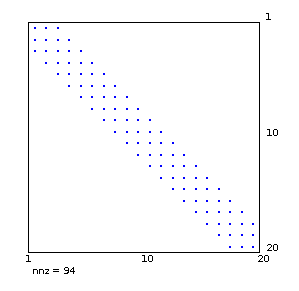
\includegraphics[scale=0.7]{figures/bound.png}
% \label{fig:bound}
% \end{figure}
% 
% Nous allons pr\'esenter trois exemples de fonction appartenant \`a la librairie; la fonction bien connue Rosenbrock, g\'en\'eralis\'ee \`a dimension variable, 
% une fonction trigonom\'etrique et une fonction utilisant les polynômes de Chebychev.
% 
% 
% 
% Comme les polynômes sont de plus en plus compliqu\'es \`a calculer quand la dimension augmente, le coût de $f$
% ne va pas être lin\'eaire par rapport \`a $n$.





\section{Pr\'ecision des objectifs}
Maintenant que nous avons pr\'esent\'e les algorithmes, nous pouvons mieux pr\'eciser les objectifs du pr\'esent travail.
Le but est d'adapter une libraire sous scilab et d'être capable d'une part de fournir les d\'eriv\'ees des fonctions qui v\'erifient
les complexit\'es expos\'ees en \ref{chap1:ordre} et d'autre part r\'esoudre les syst\`emes lin\'eaires.
La difficult\'e des m\'ethodes r\'eside dans l'ensemble des op\'erations critiques : 
\begin{itemize}
\item $\nabla f(x)$
\item $\nabla f(x)\cdot u$
\item $\nabla^2 f(x)$
\item $\nabla^2 f(x)\cdot u$
\item $\nabla^3 f(x)\cdot u$
\item $\nabla^3 f(x)\cdot u\cdot v$
\item $\nabla^4 f(x)\cdot u\cdot v \cdot w$
\item d\'ecomposition de Cholesky $LDL^T = P(A+E)P^T$
\item r\'esolution du syst\`eme $LDL^Tx =b$
\end{itemize}


{\co 
Nous voulons exploiter au mieux l'utilisation de la DA afin d'obtenir des temps de calcul raisonnable pour les d\'eriv\'ees. 
Nous allons ainsi pr\'esenter la r\'esolution des syst\`emes lin\'eaire requis par les \'equations et par cons\'equent 
la d\'ecomposition de Cholesky modifi\'ee et la r\'esolution des syst\`emes triangulaires. Bien entendu, il nous faudra
une efficacit\'e assur\'e pour que ces calculs ne soient pas un frein \`a ceux de la DA.
Puis nous analyserons les processus de la diff\'erentiation automatique dans 
l'obtention des d\'eriv\'ees. Nous verrons ainsi qu'il existe deux modes bien distincts pour les calculs et diff\'erentes techniques 
d'impl\'ementation. Puis, nous d\'etaillerons les choix au niveau des outils et des librairies pour les op\'erations critiques et leurs tests.
 Enfin, nous observerons les r\'esultats obtenus pour les temps d'ex\'ecution et l'efficacit\'e des m\'ethodes.}




{\small\center

\begin{table}[h!]
\caption{Liste des fonctions de la librairie MGH, les variables entre parenth\`eses sont modifiables.}
\center
\begin{tabular}{|r|r|r|l|}
\hline
 No & $n$ & $m$ & Nom \\
\hline
 1. &   2 &   2 &  Rosenbrock\\
 2. &   2 &   2 &  Freudenstein and Roth\\
 3. &   2 &   2 &  Powell Badly Scaled\\
 4. &   2 &   3 &  Brown Badly Scaled\\
 5. &   2 &   3 &  Beale\\
 6. &   2 &  10 &  Jennrich and Sampson\\
 7. &   3 &   3 &  Helical Valley\\
 8. &   3 &  15 &  Bard\\
 9. &   3 &  15 &  Gaussian\\
10. &   3 &  16 &  Meyer\\
11. &   3 &  10 &  Gulf Research and Development\\
12. &   3 &  10 &  Box 3-Dimensional\\
13. &   4 &   4 &  Powell Singular\\
14. &   4 &   6 &  Wood\\
15. &   4 &  11 &  Kowalik and Osborne\\
16. &   4 &  20 &  Brown and Dennis\\
17. &   5 &  33 &  Osborne 1\\
18. &   6 &  13 &  Biggs EXP6\\
19. &   11&  65 &  Osborne 2\\
20. & (20)&  31 &  Watson\\
21. & (10)& (10)&  Extended Rosenbrock\\
22. & (10)& (10)&  Extended Powell Singular\\
23. & ( 4)& ( 5)&  Penalty I\\
24. & ( 4)& ( 8)&  Penalty II\\
25. & (10)& (12)&  Variably Dimensioned\\
26. & (10)& (10)&  Trigonometric\\
27. & (10)& (10)&  Brown Almost Linear\\
28. & (10)& (10)&  Discrete Boundary Value\\
29. & (10)& (10)& Discrete Integral Equation\\
30. & (10)& (10)&  Broyden Tridiagonal\\
31. & (10)& (10)&  Broyden Banded\\
32. & (10)& (20)&  Linear --- Full Rank\\
33. & (10)& (20)&  Linear --- Rank 1\\
34. & (10)& (20)&  Linear --- Rank 1 with Zero Columns and Rows\\
35. & (10)& (10)&  Chebyquad\\
\hline
\end{tabular}
\label{tab:mgh}
\end{table}
}








%Nous verrons aussi les limitations d'un outil (Tapenade).
% \subsection{Halley}
% Complexit\'e : $C(d_N)+$ Tenseur$\times$Vecteur



% http://www.springerlink.com/content/k63463/#section=397656&page=1

% http://plato.asu.edu/sub/nlounres.html
 % fichier chapitre-1.tex

%=========================== CHAPITRE 2 ============================
\modeFrancais{}
\chapter[Calculs d'alg\`ebre lin\'eaire : inversion du hessien] 
        {\singlespacing%
         Calculs d'alg\`ebre lin\'eaire : inversion du hessien}
         \label{ch:chapitre-2}



\section{R\'esolution de syst\`eme lin\'eaire}
{\co Comme nous l'avons vu, le calcul des it\'er\'es passe par la r\'esolution de syst\`emes lin\'eaires.} Dans l'exemple de Newton,
 il faut r\'esoudre $\nabla^2 f(x)d_N=\nabla f(x)^T$ o\`u $\nabla^2 f(x^*)\in \mathbb{R}^{n\times n}$
 est une matrice sym\'etrique et $\nabla f(x)^T \in \mathbb{R}^n$.
Il s'agit donc d'un syst\`eme lin\'eaire de la forme $Ax=b$ de grande taille. Il n'est pas envisageable 
d'adopter une r\'esolution du type Cramer, pour que ce soit efficace, nous devons
 modifier la matrice $A$, il existe plusieurs d\'ecompositions:
{\co 
\subsection{Survol des d\'ecompositions classiques pour la r\'esolution}}
\begin{description}
  \item[\'Elimination de Gauss-Jordan] \hfill \\
Aussi appel\'e pivot de Gauss, elle s'applique sur une matrice $A \in \mathbb{R}^{n\times n}$ non singuli\`ere.
 La strat\'egie est de r\'eduire gr\^ace aux op\'erations \'el\'ementaires sur les colonnes de $A$ pour obtenir une matrice triangulaire sup\'erieure. 
Il y a $n-1$ \'etapes, premi\`erement, $A^{(1)}\leftarrow A$ et $b^{(1)}\leftarrow b$ sont initialis\'es. Au bout
de la $k$i\`eme \'etape, nous avons $A^{(k)}x=b^{(k)}$ %o\`u
$$A^{(k)}= \left[
\begin{array}{rl}
 A^{(k)}_{11} & A^{(k)}_{12} \\
 0       & A^{(k)}_{22} \\
\end{array}\right]$$
o\`u $A^{(k)}_{11} \in \mathbb{R}^{(k-1)\times(k-1)}$ est une matrice triangulaire sup\'erieure.

L'\'elimination de Gauss-Jordan a un coût de $\frac{2}{3}n^3$.


  \item[D\'ecomposition LU] \hfill \\
Pour une matrice $A\in \mathbb{R}^{n\times n}$, cette d\'ecomposition fournit deux matrices $LU$ o\`u
$L$ est une matrice triangulaire inf\'erieure et $U$ une matrice triangulaire sup\'erieure. Il existe une unique d\'ecomposition si
et seulement si $A_k=A(1:k,1:k)$ est non singuli\`ere pour $k=1:n-1$, sinon elle existe mais n'est pas unique.

La d\'ecomposition LU a un coût de l'ordre de $\frac{2}{3}n^3$.


  \item[D\'ecomposition de Cholesky] \hfill \\


Cette d\'ecomposition, dûe au fran\c{c}ais Andr\'e-Louis Cholesky (1875-1918 alors qu'il \'etait commandant en chef) permet de r\'esoudre de mani\`ere efficace des syst\`emes
 d'\'equation lin\'eaire de la forme $Ax=b$ lorsque $A$ est une matrice d\'efinie positive.

\begin{frtheoreme}
 Si A est une matrice r\'eelle sym\'etrique,  d\'efinie positive, alors il existe une unique matrice L
triangulaire inf\'erieure et inversible, telle que
 $$A = LL^T$$
\end{frtheoreme}



\begin{algorithm}                     % enter the algorithm environment
\caption{Factorisation de Cholesky}          % give the algorithm a caption
\label{alg:chol}                           % and a label for \ref{} commands later in the document
\begin{algorithmic}  
\STATE \textbf{Pr\'ealables:} %Variables en entr\'ee :  
\begin{itemize}
\item[$\bullet$] Soit $A \in \mathbb{R}^{n\times n}$ une matrice sym\'etrique d\'efinie positive
\end{itemize}
\STATE \textbf{En sortie:} %Variables en entr\'ee :  
\begin{itemize}
\item[$\bullet$] calcule $R$ o\`u $A=R^TR$ et $R=(r_{ij})_{1\leq i,j\leq n}$
\end{itemize}
\FOR{$j = 1:n$} 
\FOR{$i = 1:n$} 
\STATE $r_{ij}\leftarrow(a_{ij}-\sum_{k=1}^{i-1}r_{ki}r_{kj})/r_{ii}$
\ENDFOR
\STATE $r_{jj}=(a_{jj}-\sum_{k=1}^{j-1}r_{kj}^2)^{1/2}$
\ENDFOR
\end{algorithmic}
\end{algorithm}


Pour r\'esoudre le syst\`eme, $Ax = LL^Tx = b$, on commence par r\'esoudre $Ly=b$ puis $L^Tx=y$.
Le nombre d'op\'erations requis pour cette d\'ecomposition est de l'ordre de $\frac{1}{3}n^3$. Il s'agit de la m\'ethode 
la plus efficace donc celle que l'on devrait utiliser, cependant lorsque la m\'ethode de Newton est appliqu\'ee,
la matrice hessienne n'est a priori pas d\'efinie positive. C'est pour cette raison que l'algorithme de Cholesky a \'et\'e 
modifi\'e. La matrice va être corrig\'ee pour obtenir une d\'ecomposition d\'efinie positive
 et plutôt bien conditionn\'ee.
\end{description}


\subsection{D\'ecomposition de Cholesky Modifi\'ee}
\label{chap1:decomposition}

Soit une matrice $A$, sym\'etrique mais pas n\'ecessairement d\'efinie positive. L'algorithme de Cholesky modifi\'ee
calcule la d\'ecomposition $P(A+E)P^T=LDL^T$ o\`u $P$ est une matrice de permutation, $E$ est une
perturbation pour rendre la matrice $A+E$ d\'efinie positive, $D$ est une matrice diagonale et 
$L$ une matrice triangulaire inf\'erieure. La norme de $E$ devrait être petite et $A+E$ 
bien conditionn\'ee. Cette technique est largement utilis\'ee en optimisation comme dans notre cas ou bien pour 
calculer des pr\'e-conditionneurs d\'efinis positifs.
Comme le soulignent Cheng et Higham dans \cite{Higham}, les objectifs de l'algorithme de Cholesky modifi\'e peuvent être d\'eclar\'es
comme suit :
\begin{itemize}
\item[O1] Si $A$ est "suffisamment d\'efinie positive", alors $E$ devrait être \'egale \`a z\'ero.
\item[O2] Si $A$ est ind\'efinie, $\lVert E \rVert$ ne devrait pas être plus grand que 
\[\min\{\lVert \Delta A \rVert: A+\Delta A \text{ est d\'efinie positive } \} \]
pour une norme appropri\'ee.
\item[O3] La matrice $A+E$ devrait être raisonnablement bien conditionn\'ee. 
\item[O4] Le coût de l'algorithme devrait être le même que le coût de la d\'ecomposition standard de Cholesky
 pour l'ordre le plus \'elev\'e.
\end{itemize}



  \section{Utilisation de la d\'ecomposition de Cholesky modifi\'ee}

\label{chap3:cholesky}

Il existe plusieurs versions de la d\'ecomposition de Cholesky modifi\'ee en Scilab mais pas 
de version efficace. Cela est li\'e intrins\`equement \`a {\it Scilab} qui est un langage de haut niveau et n'est pas performant pour effectuer du code
imp\'eratif sur des grandes dimensions comparativement au C ou Fortran.
Par cons\'equent, nous avons choisi deux routines appartenant \`a Lapack\footnote{\url{http://www.netlib.org/lapack/}}, une libraire sur les syst\`emes lin\'eaires \'ecrite en fortran.
 La premi\`ere permet la d\'ecomposition 
de Cholesky modifi\'ee et la deuxi\`eme la r\'esolution du syst\`eme avec cette d\'ecomposition, nomm\'ee {\tt dsytrf} et {\tt dsytrs} respectivement. 
Cette d\'ecomposition de Cholesky modifi\'ee utilise la m\'ethode de pivotement de Bunch-Kaufman (BK) \cite{Bunch}.

Soit une matrice $A \in \mathbb{R}^{n\times n}$ non nulle, la factorisation fournit $$P(A+E)P^T=L(D+F)L^T.$$ $F$ est choisie pour que $D+F$ et ainsi
$A+E$ soient d\'efinies positives. Cette technique a \'et\'e propos\'ee par Mor\'e et Sorensen \cite{More}. L'id\'ee consiste \`a 
trouver une permutation $\Pi$ et un entier $s=1$ ou $2$ tel que 

\begin{equation*}
\Pi A \Pi^T = 
\left[
\begin{array}{cc}
 E & C^T \\
 C & B \\
\end{array}\right]
\end{equation*}
avec $E\in \mathbb{R}^{s\times s}$ non singuli\`ere et $B\in \mathbb{R}^{(n-s)\times (n-s)}$. En choisissant correctement $\Pi$, nous avons la factorisation :

\begin{equation*}
\Pi A \Pi^T = 
\left[
\begin{array}{cc}
 I_s & 0 \\
 CE^{-1} & I_{n-s} \\
\end{array}\right]
\left[
\begin{array}{cc}
 E & 0 \\
 0 & B-CE^{-1}C^T \\
\end{array}\right]
\left[
\begin{array}{cc}
 I_s & E^{-1}C^T \\
 0 & I_{n-s} \\
\end{array}\right]
\end{equation*}
Le proc\'ed\'e est r\'ep\'et\'e r\'ecursivement sur la matrice $S=B-CE^{-1}C^T$ de taille\\ $(n-s)\times (n-s)$. On remarque ainsi qu'au lieu
d'utiliser un pivot de taille $1\times 1$, on peut utiliser une matrice $2\times2$.




 Selon Cheng et Higham \cite{Higham}, l'algorithme de BK, que celui de Schnabel et Heskow \cite{choleskymod}, a un coût identique
 \`a la d\'ecomposition de Cholesky standard relativement
aux termes d'ordre les plus \'elev\'es, cependant les objectifs O1 et O3 de la partie \ref{chap1:decomposition} sont difficilement satisfaits.
Il se peut que la matrice $A+E$ soit mal conditionn\'ee car $\lVert L \rVert_{\infty}$ n'est pas born\'ee et par cons\'equent les valeurs propres de $D$ peuvent 
largement diff\'erer de $A$. 
Les auteurs proposent ainsi une autre version de l'algorithme de BK, permettant de satisfaire les conditions mais nous consid\'ererons que 
les routines de lapack permettrons d'obtenir des directions satisfaisantes d'autant plus que nous utiliserons une recherche lin\'eaire ce qui injectera
un niveau de contrôle en plus.

Afin d'obtenir une matrice d\'efinie positive, nous profitons de cette d\'ecomposition pour changer les \'el\'ements diagonaux.
L'avantage, c'est que l'on a plus besoin de faire ces changements sur une matrice $n$ par $n$ mais seulement $2\times2$ ou $1\times1$.

\begin{algorithm}                     % enter the algorithm environment
\caption{Changement de la diagonale}          % give the algorithm a caption
\label{alg:diag}                           % and a label for \ref{} commands later in the document
\begin{algorithmic}
\STATE \textbf{Pr\'ealables:} %Variables en entr\'ee :  
\begin{itemize}
\item[$\bullet$] $\epsilon>0$
\item[$\bullet$] $\Tilde{D}$ la matrice diagonale par bloc
\end{itemize}
\STATE \textbf{Sortie} %Variables en entr\'ee :  
\begin{itemize}
\item[$\bullet$] $D$ la matrice diagonale par bloc avec pour valeur 
propre minimale $\lambda_{min} \geq \epsilon$
\end{itemize}

\STATE Pour chaque bloc de la diagonale $\Tilde{D_k}$,
\IF{$\Tilde{D_k}$ est de dimension $1\times1$}
\STATE $D_k\leftarrow \max(\Tilde{D_k},\epsilon)$
\ELSE 
%\COMMENT{$D$ est de dimension $2\times2$} 
\STATE $[Z,W]=spec(\Tilde{D_k)}$
\COMMENT{Il s'agit de la diagonalisation de $\Tilde{D_k}$ : $ZWZ^T=\Tilde{D_k}$ avec $W$ matrice diagonale}
\STATE $D_k\leftarrow Z*diag(max(diag(W),\epsilon))*Z^T$
\ENDIF
\end{algorithmic}
\end{algorithm}


% function D=moddiag(D,Ipiv)
% [nr,n]=size(D);
% eps=0.00001
% 
% first(1)=%t
% for j=1:n-1
% 	    if(Ipiv(j)<0 & first(j)) then first(j+1)=%f, D(j,j+1)= D(j+1,j)
% 	    else first(j+1)=%t
% 	    end
% end
% for i=1:n
%       if(first(i)) then
% 	  if(Ipiv(i)<0) then
% 	      [Z,W]=spec(D(i:i+1,i:i+1));
% 	      D(i:i+1,i:i+1)=Z*diag(max(diag(W),eps))*Z'
% 	      else D(i,i)=max(D(i,i),eps)
% 	  end
%       end
% end
% endfunction
% eps=0.00001
% A=rand(2,2)
% A=A+A'
% [Z,W]=spec(A)
% A2=Z*diag(max(diag(W),eps))*Z'



\section{R\'esolution des syst\`emes lin\'eaires}

\label{chap2:decomp}
Pour commencer, il est \`a noter que la r\'esolution 
des syst\`emes triangulaires dans {\it Scilab} n'est g\'en\'eralement pas efficace. Il s'av\`ere que la d\'etection du syst\`eme triangulaire 
n'est pas faite syst\'ematiquement. La figure \ref{fig:lu} r\'ev\`ele que sur les quatre tests de r\'esolution
 $Lx=e$, $L'x=e$, $U'x=e$, $Ux=e$ o\`u $L$ et $U$ proviennent de la d\'ecomposition $LU$ r\'ealis\'e par {\it Scilab} et
 $e=(1)_{1\leq i\leq n}$ un vecteur colonne, une seule est performante.

\begin{figure}
\caption{R\'esolution d'un syst\`eme triangulaire par {\it Scilab} avec une d\'ecomposition LU, sur les quatre versions,
qu'une seule n'est efficace.}
\center
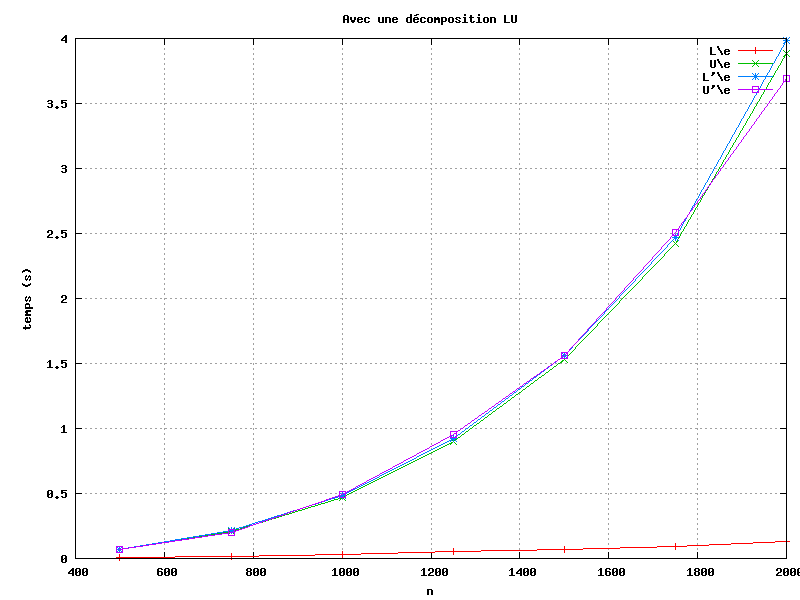
\includegraphics[scale=0.39]{figures/LU.png}
\label{fig:lu}
\end{figure}


\begin{figure}
\caption{R\'esolution d'un syst\`eme triangulaire par {\it Scilab} avec une d\'ecomposition de Cholesky}
\center
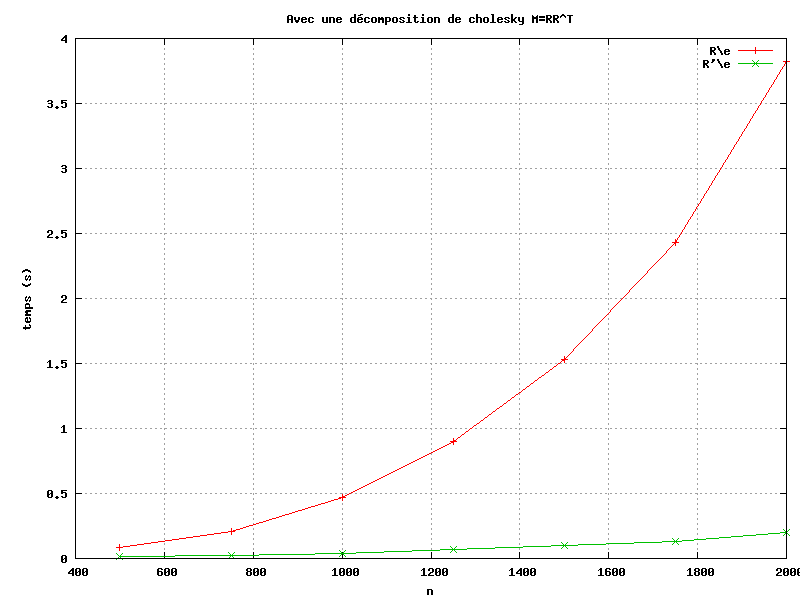
\includegraphics[scale=0.39]{figures/chol.png}
\label{fig:chol}
\end{figure}

C'est pour cette raison que nous avons pr\'ef\'er\'e choisir une d\'ecomposition \'ecrite en fortran pour nos calculs.


La r\'esolution des syst\`emes $Ax=b$ s'effectue en trois temps. Tout d'abord, $A$ qui est par exemple 
la hessienne de notre fonction, est d\'ecompos\'ee en

 $$L\Tilde{D}L^T=P^T(A+E)P$$ o\`u $D$ est une matrice diagonale par bloc soit de taille $1\times 1$, soit $2\times 2$.
 La factorisation a un coût de $\frac{1}{3}n^3$. Ensuite, on modifie chacun de ces blocs
pour le rendre d\'efini positif : $D\leftarrow \Tilde{D}+\Delta \Tilde{D}$. Cette op\'eration est 
de l'ordre de $n$ mais elle est effectu\'ee avec {\it Scilab}
 Enfin, on r\'esout le syst\`eme $LDL^Tx=b$ qui est une op\'eration en $n^2$.








\subsection{Temps de calcul de l'ensemble de la r\'esolution}


Comme le montre la figure \ref{fig:temps8}, la factorisation modifi\'ee est l'op\'eration qui prend le plus de temps,
elle a un comportement en $n^3$. La r\'esolution du syst\`eme lin\'eaire est plus rapide que le changement de la 
diagonale parce qu'elle est ex\'ecut\'ee en fortran.
\begin{figure}
\caption{R\'esolution du syst\`eme $Ax=b$ avec la factorisation de Cholesky modifi\'ee}
\center
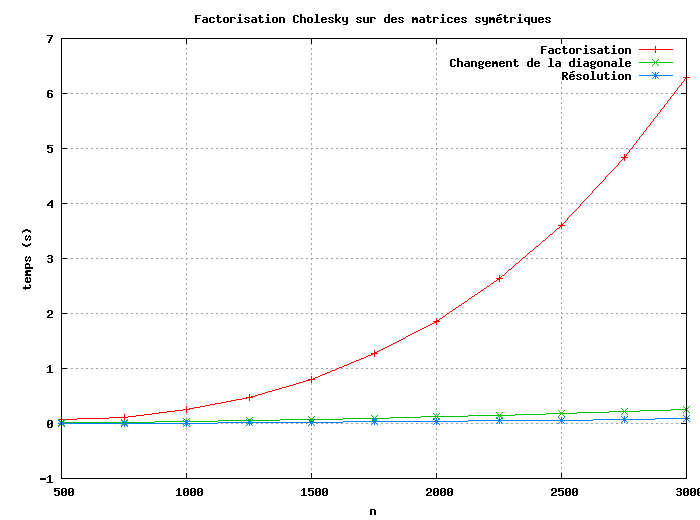
\includegraphics[scale=0.4]{figures/temps8.png}
\label{fig:temps8}
\end{figure}


\begin{table}[h]
	\begin{center}
\begin{tabular}{|c|c|c|c|c|}\hline
n & D\'ecomposition & Arrangement & R\'esolution & $A \backslash b$ avec Scilab\\
 & $A\leftarrow LDL^T$ & $D\leftarrow \Tilde{D}+\Delta \Tilde{D}$& $Lu=b$, $\Tilde{D}v=u$, $L^Tx=v$ & \\
\hline
$500 $&$  0.037000 $&$  0.011000 $&$ 0.002000 $&$ 0.090000$\\\hline
$750 $&$ 0.122000 $&$ 0.026000 $&$ 0.005000 $&$ 0.220000$\\\hline
$1000 $&$ 0.254000 $&$ 0.038000 $&$ 0.010000 $&$ 0.486000$\\\hline
$1250 $&$ 0.475000 $&$ 0.055000 $&$ 0.015000 $&$ 0.944000$\\\hline
$1500 $&$ 0.809000 $&$ 0.075000 $&$ 0.022000 $&$ 1.607000$\\\hline
$1750 $&$ 1.278000 $&$ 0.097000 $&$ 0.030000 $&$ 2.543000$\\\hline
$2000 $&$ 1.863000 $&$ 0.123000 $&$ 0.038000 $&$ 3.732000$\\\hline
$2250 $&$ 2.636000 $&$ 0.149000 $&$ 0.047000 $&$ 5.413000$\\\hline
$2500 $&$ 3.602000 $&$ 0.179000 $&$ 0.057000 $&$ 7.402000$\\\hline
$2750 $&$ 4.830000 $&$ 0.215000 $&$ 0.070000 $&$ 10.116000$\\\hline
$3000 $&$ 6.320000 $&$ 0.251000 $&$ 0.084000 $&$ 13.327000$\\\hline
\end{tabular}
	\end{center}
	\caption{Temps de calcul en seconde pour chaque \'etape de la r\'esolution du syst\`eme $Ax=b$, bien que la modification de la diagonale soit
$\mathcal{O}(n)$, elle est moins efficace que la r\'esolution car elle est cod\'ee en {\it Scilab}.}
	\label{tab:newton}
\end{table}



{\co 
\subsection{Conclusion}
Nous venons d'obtenir une interface reliant {\it Scilab} \`a {\it Fortran} nous permettant d'obtenir
une r\'esolution de syst\`emes lin\'eaire de mani\`ere efficace et ce même si la matrice n'est pas d\'efinie 
positive. 
\`A pr\'esent, nous allons nous interesser \`a la diff\'erentition automatique, les probl\`ematiques qu'elle
soul\`eve et diff\'erents modes qui existent. Nous verrons plus tard si les outils sont suffisamment performants
pour valider les bornes de complexit\'e d\'efinies dans le chapitre 1.
}




 % fichier chapitre-2.tex
% 

%=========================== CHAPITRE 3 ============================
\modeFrancais{}
\chapter[Obtention des d\'eriv\'ees : Diff\'erentiation automatique] 
        {\singlespacing%
         Obtention des d\'eriv\'ees : Diff\'erentiation automatique}
         \label{ch:chapitre-3}


\section{Introduction}
{\co Comme le souligne Corliss \cite{Corliss1991b}, la DA est une technique introduite vers 1962 avec le mode direct mais n'a pas r\'eussi \`a s'imposer.
 Ce n'est que plus tard, en 1982, grâce \`a l'am\'elioration des techniques de programmations et l'introduction du mode inverse que la DA a
 connu plus de succ\`es.
Griewank est \`a l'origine de grands progr\`es et il s'en ait suivi une forte augmentation du nombre d'outils, de techniques et d'applications 
de la diff\'erentiation automatique. 
L'implantation de la DA se divise en deux formes : la surcharge des op\'erateurs et la transformation du code.
La surcharge des op\'erateurs consitent \`a \'etandre la s\'emantique des op\'erations, c'est-\`a-dire que chaque variable est surcharg\'ee
par sa d\'eriv\'ee et les op\'erations s'op\`erent ces les deux quantit\'es. }
La tranformation de code, ne fait que retourner le code de la d\'eriv\'ees. Le code est analys\'e puis transformer, en fait les lignes 
correspondant au calcul de la diff\'erenti\'ee sont rajout\'ees. Ce code est parfois \'ecrit \`a la main mais la DA a suffisamment fait de progr\`es pour g\'en\'erer un code en quelques minutes (pour les gros programmes) et 
d'une qualit\'e comparable d'apr\`es l'article \cite{diffautoopa}.

 Nous verrons ainsi quelles sont les points forts et faibles de ces deux
proc\'ed\'es.



% --------------------- \`a am\'eliorer -------------------------------
% Il existe deux formes diff\'erentes de DA. Soit par transformation de code, qui analyse le code original pour produire le 
% code de la diff\'erenti\'ee ; le code adjoint. Il est parfois \'ecrit
% \`a la main mais la DA a suffisamment fait de progr\`es pour g\'en\'erer un code en quelques minutes (pour les gros programmes) et 
% d'une qualit\'e comparable d'apr\`es l'article \cite{diffautoopa}.
% Soit la surcharge des op\'erateurs qui consiste \`a sp\'ecifier les calculs de 
% d\'erivation associ\'es \`a chaque op\'eration effectu\'ee.
% --------------------- \`a am\'eliorer -------------------------------


% explication de la diff\'erentiatation automatique : diff\'erence avec la
% diff\'erentiation symbolique et par diff\'erences finies
%

Ainsi, comme indiqu\'e dans \cite{differentiaauto}, le but de la DA est de calculer la d\'eriv\'ee d'une fonction sp\'ecifi\'ee par
un programme, un algorithme. Cette m\'ethode de calcul s'oppose \`a deux autres
bien connues : la diff\'erentiation symbolique et la diff\'erentiation par
diff\'erences finies. La premi\`ere, que l'on peut retrouver dans {\it Maple}, 
utilise l'expression de la fonction pour d\'eterminer sa d\'eriv\'ee.
Cette technique est tr\`es vite limit\'ee d'une part lorsque l'on a des
expressions un peu complexes et d'autre part parce qu'il faut l'expression de la
fonction. \\
Par exemple sur {\it Maple}, si on veut obtenir :
\[\frac{\partial^3((x^2+y^2)*(\ln(x)-\ln(y)))}{\partial y \partial^2x}\]
\verb!diff((x^2+y^2)*(ln(x)-ln(y)), y,x$2);!\\
$\rightarrow$ $-\frac{2y}{x^2}-\frac{2}{y}$
\\
%

{\co
Griewank illustre un exemple de diff\'erentiation symbolique dans \cite{Iri89onautomatic}, avec le logiciel {\it Macsyma}. La fonction
qui permet de calculer l'energie d'Helmholtz est fournie au logiciel. Le r\'esultat correspond \`a la figure \ref{fig:macsyma}. 
En plus du fait que le code g\'en\'er\'e est difficilement comprehensible pour un être humain, le code a du être modifi\'e \`a cause 
du maximum de 19 lignes cons\'ecutives en Fortran. Ainsi, il est extrêment difficile de pouvoir maintenir une telle structure de code.
}

\begin{figure}
\caption{Code produit par diff\'erentiation symbolique \`a partir du logiciel {\it Macsyma}}
\begin{center}
\fbox{
\begin{minipage}[c]{0.7\textwidth}
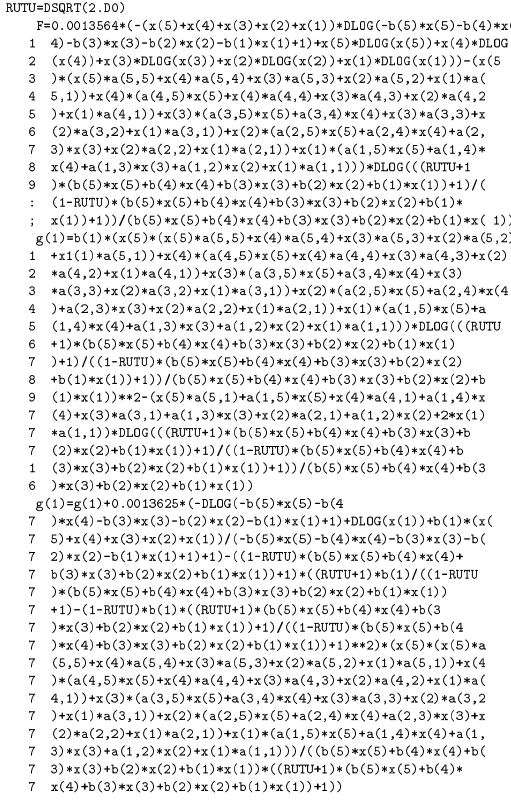
\includegraphics[scale=0.7]{figures/macsyma.png}
\end{minipage}
}
\end{center}
\label{fig:macsyma}
\end{figure}


% 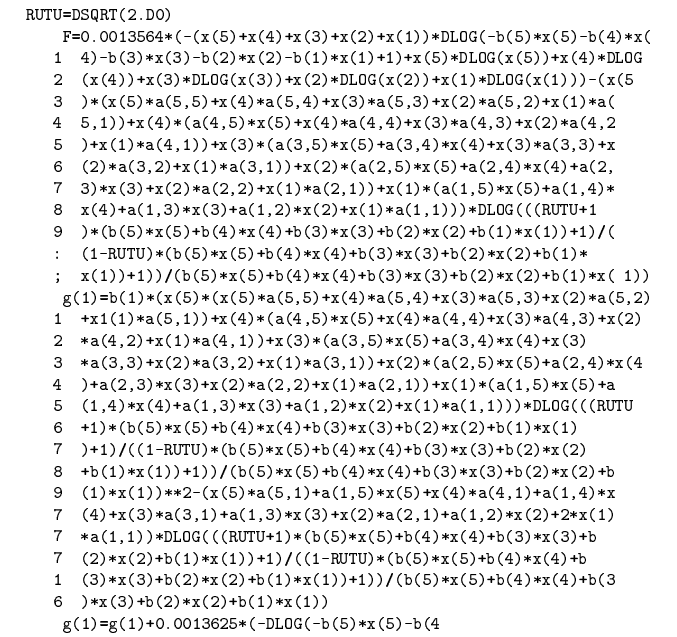
\includegraphics[scale=0.5]{figures/macsyma1.png}\\
% 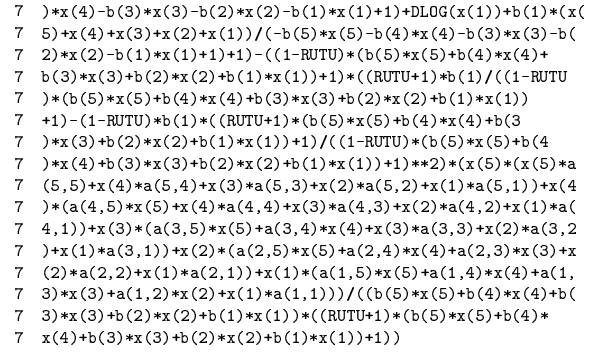
\includegraphics[scale=0.5]{figures/macsyma2.png}\\

La  plupart du temps, il faut diff\'erentier un code constitu\'e de
boucles et de conditions qui est difficilement exprimable par une expression
math\'ematique.
 La diff\'erentiation num\'erique ou par diff\'erences finies
s'appuie sur l'expression th\'eorique de la d\'eriv\'ee: 
$$\lim_{h\rightarrow 0}\frac{f(x+h)-f(x)}{h}$$
Dans le cas \`a plusieurs dimensions:
$$\lim_{\varepsilon \rightarrow 0}\frac{P(X+\varepsilon \cdot dX)-P(X)}{\varepsilon} =
 \nabla P(X)\cdot dX$$
Cependant, il s'agit d'un probl\`eme hasardeux \`a cause de la
discr\'etisation impos\'ee par ordinateur. $h$ doit être choisi dans l'ordre de
 grandeur de la racine de la pr\'ecision machine : si $h$ est trop proche de $0$ la
diff\'erence va être mal approch\'ee ; l'\'ecart entre $f(x+h)$ et $f(x)$
 \'etant trop faible et si $h$ est trop grand, on s'\'eloigne de la v\'eritable
valeur de la d\'eriv\'ee. Ainsi, nous allons voir que la diff\'erentiation
automatique pallie \`a ces deux inconv\'enients majeurs. \\






\section{Principes de la diff\'erentiation automatique}
\label{sec:da}

{\co Contrairement \`a la diff\'erentiation symbolique, l'objectif de la diff\'erentiation automatique n'est pas de concevoir l'expression de la d\'eriv\'ee mais uniquement
le programme qui la calcule.}
La DA calcule la d\'eriv\'ee de mani\`ere analytique, c'est-\`a-dire qu'elle obtient le calcul exact de la d\'eriv\'ee. Ainsi, il n'y a pas d'erreurs
d'approximations. \`A chaque fois qu'appara\^it une variable dans le programme source,
le programme diff\'erenti\'e va calculer une variable additionnelle de la même forme : sa diff\'erenti\'ee.
Il est \`a noter que la DA ne vise pas \`a fournir l'expression math\'ematique de la d\'eriv\'ee, puisqu'elle ne fournit que du
code permettant son \'evaluation.
Il existe deux mani\`eres d'utiliser la DA, soit le code est transform\'e pour obtenir un nouveau programme qui
calculera directement la diff\'erenti\'ee, soit par surcharge des op\'erateurs. Nous allons d\'ecrire en d\'etail ces diff\'erentes approches.
Pour la deuxi\`eme approche, il s'agit d'ajouter aux fonctions de base (l'addition, cos, log) les op\'erations de d\'erivations.

Par exemple, en prenant {\tt x}, {\tt y}, {\tt z} comme variables et {\tt V} comme vecteur,
lors de l'instruction :\\
$${\tt x= y*V(10)+z}$$\\
le programme diff\'erenti\'e va  calculer :
$$\dot{\tt x}= \dot{\tt y}*{\tt V(10)} + {\tt y}*\dot{\tt V}{\tt(10)}+\dot{\tt z} $$
en utilisant les r\`egles de d\'erivations usuelles sur les fonctions. Il n'y a plus
d'approximations, c'est un calcul exact. 
Le principe est de consid\'erer que chaque programme peut s'\'ecrire comme une s\'equence
d'instructions.
$$I_1;I_2;...;I_{p-1};I_{p}$$
Cette suite peut être identifi\'ee comme une composition de fonctions 
$$f=f_p\circ f_{p-1} \circ \cdots \circ f_1$$
par la r\`egle de d\'erivation sur la composition~(\ref{annexe:A}) on obtient :\\

\begin{align*}
f'(X) = & (f'_p\circ f_{p-1} \circ f_{p-2} \circ ... \circ f_1(X))\\
& . (f'_{p-1} \circ f_{p-2} \circ ... \circ f_1(X))\\
& \cdots\\
& . f'_1(X)\\
= & f'_p(W_{p-1}) . f'_{p-1}(W_{p-2}) . \cdots .f'_1(W_0).\\
\end{align*}
En notant $W_0=X$ et $W_k=f_k(W_{k-1})$.
%
Comme plusieurs donn\'ees sont trait\'ees, tous les $f'_k$ sont des matrices Jacobiennes de 
taille relativement grande dans un cas g\'en\'eral. Calculer la diff\'erenti\'ee revient \`a calculer
les multiplications de ces matrices. Cependant, il n'est pas possible de calculer ce produit avec un co\^ut 
raisonnable. Par exemple, avec dix variables, si on effectue une quinzaine d'instructions
cela revient \`a faire de l'ordre de $10^4$ op\'erations. La complexit\'e est exponentielle. Dans la plupart
des cas, l'application qui utilise $\nabla f(X)$  n'a en r\'ealit\'e que besoin d'une direction de la jacobienne :
 $\nabla f(X).\dot{X}$ pour une certain vecteur $\dot{X}$.
Nous allons voir les deux modes de diff\'erentiation, le mode tangent et le mode inverse. Dans le premier mode, 
les calculs de la fonctions se propagent parall\`element aux d\'eriv\'ees tandis que dans le mode inverse, le calcul
s'effectue \`a rebours en partant de la fin du code.







    \subsection{Mode tangent ou mode direct}

\label{chap2:tangent}
Dans notre cas, comme par exemple pour la direction de Chebychev, nous avons besoin de calculer $\nabla^3f(x)\cdot u\cdot v$ et non $\nabla^3f(x)$.
 En prenant cela en compte, le calcul va être largement simplifi\'e. \`A l'ordre un : $\dot{Y}=f'(X).\dot{X}$
$$\dot{Y}=f'_p(W_{p-1}) . f'_{p-1}(W_{p-2}) . \cdots .f'_1(W_0).\dot{X}.$$\\
Pour profiter de la multiplication avec le vecteur, le calcul va se faire de droite \`a gauche afin d'\'eviter d'avoir des multiplications de 
Matrice$\times$Matrice (correspond au mode multi-directionnel pour Tapenande) mais plut\^ot Matrice$\times$Vecteur. De plus, de cette mani\`ere, les appels aux $W_i$ vont
se faire dans l'ordre, donc en même temps qu'ils seront calcul\'es. Cette m\'ethode donne une combinaison lin\'eaire des 
colonnes de la matrice Jacobienne.
Voici un exemple illustr\'e pour la fonction $f(x_1,x_2)=(x_1-cos(x_2))^2$. Dans le Graphe Acyclique Orient\'e \ref{fig:gao}, le 
gradient de chaque quantit\'e en partant des feuilles va être propag\'e.


\begin{figure}
\caption{GAO : $f(x_1,x_2)=(x_1-cos(x_2))^2$ pour \'evaluer la fonction, le parcours se fait 
\`a partir des feuilles de l'arbre jusqu'\`a la racine.}
\begin{center}
\fbox{
\begin{minipage}[c]{0.45\textwidth}
\beginpgfgraphicnamed{figures/figure_14}
\endpgfgraphicnamed
\end{minipage}
}
\end{center}
\label{fig:gao}
\end{figure}




% \floatstyle{ruled}
% \newfloat{Program}{tbp}{lop}[section]
% \begin{Program}
% \begin{verbatim}
% . . . program text . . .
% \end{verbatim}
% \caption{. . . caption . . . }
% \end{Program}








\begin{figure}
\caption{GAO : mode tangent, il suit le même parcours que celui de l'\'evaluation}
\begin{center}
\fbox{
\begin{minipage}[c]{0.6\textwidth}
\beginpgfgraphicnamed{figures/figure_11}
\endpgfgraphicnamed
\end{minipage}
}
\end{center}
\label{fig:modetangent}
\end{figure}



\vspace{1cm}
\begin{tabular}{|l|c|l|c|c|}
  \hline
  $y$ & Valeurs de $y$ & $\dot{y}$ & Valeurs de $\dot{y}$ & Valeurs vectorielles
\\
  \hline
  $y_1$ &  $x_1$ &  $\dot{y_1}$ & $\dot{x_1}$ & [$1$ \ $0$] \\
  $y_2$ & $x_2$ & $\dot{y_2}$ & $\dot{x_2}$ & [$0$ \ $1$] \\
  $y_3$ & $cos(y_2)$ & $\dot{y_3}$ & $-\dot{y_2}sin(y_2)$ & -[$0$ \ $sin(x_2)$]
\\
  $y_4$ & $y_1-y_3$ & $\dot{y_4}$ & $\dot{y_1}-\dot{y_3}$ & [$1$ \ $sin(x_2)$]
\\
  $y_5$ & $y_4^2$ &  $\dot{y_5}$ & $2\dot{y_4}y_4$ & $2$[$x_1-cos(x_2)$ \
$(x_1-cos(x_2))sin(x_2)$]\\
  
  \hline
\end{tabular}



\vspace{1cm}

Le programme g\'en\'er\'e par la DA \'evalue simultan\'ement la fonction et le gradient. Le nombre de lignes obtenu
est environ deux fois celui du programme d'origine puisque chaque affectation est accompagn\'ee du calcul du
gradient. En g\'en\'eral, comme c'est expliqu\'e dans \cite{Iri89onautomatic}, le mode tangent multiplie le nombre
 d'op\'erations arithm\'etiques de $n$. Chaque quantit\'e 
$x_i$ est pr\'ec\'ed\'ee du calcul de $\nabla x_i$ de taille $n$. Dans l'exemple, on peut observer que les quantit\'es propag\'ees ont 
une dimension \'equivalente au nombre de composante de l'argument. Ainsi, le coût dû au calcul du gradient est de l'ordre de 
$n$ fois le co\^ut de l'\'evaluation de la fonction.
\vspace{0.51cm}



% \end{figure}

% 

    \subsection{Mode inverse}
{\co Comme nous venons de le voir, le mode tangent propage un vecteur de la taille du gradient dans le graphe, par cons\'equent, le coût 
est proportionnel \`a $n\#(f)$. En revanche, le mode inverse ne va que propager un scalaire dans le graphe mais le parcours va se faire dans le 
sens inverse \`a celui de l'\'evaluation. C'est parce que les calculs ne se font que sur un scalaire que le coût du gradient est proportionnel
 au coût de l'\'evaluation de la fonction. 
Ainsi, il va être pr\'ef\'erable de choisir le mode inverse au mode tangent.}

Le mode inverse va nous permettre d'obtenir une ligne de la Jacobienne c'est-\`a-dire un gradient par rapport \`a 
une composante $k$.
$$\overline{X}=f'^T(X).\overline{Y}$$ 
\begin{equation}\overline{X}=f_{1}^{'T}(W_{0}) . f_{2}^{'T}(W_{1}) . \cdots .f_p^{'T}(W_{p-1}) . \overline{Y}
\label{eq:inv}
\end{equation}
L'id\'ee sous-jacente est l'utilisation des quantit\'es adjointes :

$$y_i^*= \frac{\partial f}{\partial y_i} $$
% $$y_j^*= \sum \frac{\partial f}{\partial y_j}y_i^*$$
$$\bar{y_j}= \sum_{i \in I_j} \frac{\partial f}{\partial y_j}\bar{y_i}$$
% $$\text{ o\`u tous les }\bar{y_i}\text{ sont des quantit\'es scalaires }$$
o\`u tous les $\bar{y_i}$ sont des quantit\'es scalaires
 $$I_j=\{i | y_j \text{ intervenant dans } y_i\}.$$


Le parcours du GAO se fait en profondeur, de la racine jusqu'aux feuilles. Contrairement au mode tangent,
comme les quantit\'es propag\'ees sont des scalaires, qu'une seule \'equation n'est impliqu\'ee \`a chaque n\oe ud,
 au lieu d'en avoir $n$, la dimension. Comme l'indique la figure \ref{fig:modeinverse}, les quantit\'es $\bar{y_i}$ se
propagent \`a rebours, dans le sens inverse des quantit\'es $\dot{y_i}$. C'est le fait
que le calcul se propage sur l'ensemble des feuilles qui va permettre de reconstruire le gradient de dimension $n$, chaque feuille
correspondant \`a une composante.
Commençons par observer ce mode sur notre exemple. Cette fois-ci, le parcours n'est plus le même que 
l'\'evaluation de la fonction.


\begin{figure}
\caption{GAO : mode inverse, cette fois-ci, l'arbre est parcouru depuis la racine.}
\begin{center}
\fbox{
\begin{minipage}[c]{0.75\textwidth}
\beginpgfgraphicnamed{figures/figure_12}
\endpgfgraphicnamed
\end{minipage}
}
\end{center}
\label{fig:modeinverse}
\end{figure}


\vspace{1cm}
\begin{tabular}{|l|c|}
  \hline
  $y$ & Valeurs de $y$ \\
  \hline
  $y_1$ & $x_1$ \\
  $y_2$ & $x_2$ \\
  $y_3$ & $cos(y_2)$ \\
  $y_4$ & $y_1-y_3$ \\
  $y_5$ & $y_4^2$ \\
  \hline
\end{tabular}
\hspace{1cm}
\begin{tabular}{|l|c|c|}
  \hline
 $\bar{y}$ & Valeurs de $\bar{y}$ & Valeurs \\
  \hline
 $\bar{y_5}$ & $1$ & $1$ \\
 $\bar{y_4}$ & $2y_4$ & $2(x_1-cos(x_2))$ \\
 $\bar{y_3}$ & $-\bar{y_4}$ & $2(cos(x_2)-x_1)$ \\
 $\bar{y_2}$ & $-\bar{y_3}sin(x_2)$ & $2(x_1-cos(x_2))sin(x_2)$ \\
 $\bar{y_1}$ & $\bar{y_4}$ & $2(x_1-cos(x_2))$ \\
  \hline
\end{tabular}\\

\noindent
%D'apr\`es Griewank \ref{Iri89onautomatic}, {\bf le co\^ut d'\'evaluation du gradient n\'ecessite jamais plus cinq fois le co\^ut de l'\'evaluation de la fonction}.
Dans l'\'equation \ref{eq:inv}, l'op\'eration doit se faire encore de droite \`a gauche pour que le calcul soit efficace. Malheureusement, cette fois-ci,
nous n'avons pas les appels aux $W_i$ dans le même ordre qu'ils sont calcul\'es; cela vient du fait que le parcours
n'est plus dans le même sens. Dans l'exemple, \`a la deuxi\`eme \'etape, la 
quantit\'e $y_4$ est n\'ecessaire, elle fait intervenir $y_1$ et $y_2$ alors que ces \'etats n'ont pas encore \'et\'e parcourus.
Ainsi, il existe deux strat\'egies pour obtenir les $W_i$. Soit on recalcule toutes les quantit\'es, soit on les m\'emorise toutes.




    \subsection{Strat\'egies de la DA pour le mode inverse}
% point noir stockage
% point blanc
% 
% $\overline{I_k} \rightarrow \overline{W_{k-1}}=f_k^{'T}(W_{k-1}).\overline{W_k}$
% 
\label{subsection:strategies}
 \paragraph{Recompute-All}
%  \\
Pour chaque terme $W_p=f_k(W_{p-1})$, on recalcule l'ensemble de la suite $W_i$ \`a chaque fois. L'op\'eration $W_1 =f'(X)$ va être effectu\'ee $p$ fois.
 Cette m\'ethode demande plus de temps d'ex\'ecution puisque les termes ne sont pas m\'emoris\'es, les mêmes 
calculs sont effectu\'es plusieurs fois. {\co Sur les figures commençant \`a \ref{fig:ra} jusqu'\`a \ref{fig:checkpointsa}}, les points noirs repr\'esentent le stockage de $W_k$ sur la pile
d'ex\'ecution et les points blancs repr\'esentent un d\'epilement.


% \vspace{1cm}
\begin{figure}
\caption{Strat\'egie RA : pour chaque quantit\'e \`a calculer, on reparcours le graphe pour faire un pas dans l'algorithme inverse. Prend moins de place mais
plus de temps.}
\fbox{
\begin{minipage}[c]{0.9\textwidth}
\beginpgfgraphicnamed{figures/figure_3}
\endpgfgraphicnamed
\end{minipage}
}
\label{fig:ra}
\end{figure}
% \vspace{1cm}


 \paragraph{Store-All}
Cette fois-ci, tous les termes vont être calcul\'es et enregistr\'es une seule fois. Il s'agit d'une
m\'ethode qui n\'ecessite plus de m\'emoire. Le co\^ut en m\'emoire est lin\'eaire par rapport \`a $p$.


% \vspace{1cm}
\begin{figure}
\caption{Strat\'egie SA : le graphe des \'evaluations est parcouru une seule fois pour toutes les m\'emoriser, l'algorithme inverse n'aura plus qu'\`a d\'epiler. Prend
moins de temps mais plus de capacit\'e de stockage.}
\begin{center}


\fbox{
\begin{minipage}[c]{0.9\textwidth}
\beginpgfgraphicnamed{figures/figure_4}
\endpgfgraphicnamed
\end{minipage}
}

% \beginpgfgraphicnamed{figures/figure_4}
% \endpgfgraphicnamed

\end{center}
\label{fig:sa}
\end{figure}
% \vspace{1cm}



Dans les deux cas, si le probl\`eme a une dimension trop grande, ni la strat\'egie RA, ni la SA ne pourra être
efficace. Une m\'ethode alternative appara\^it comme un bon compromis : le {\it Checkpointing}.
L'id\'ee est de d\'ecomposer le programme en plusieurs parties, si possible imbriqu\'ees et d'effectuer une sauvegarde, un {\it snapshot},
des quantit\'es entre chaque. Encore peu de travail a \'et\'e effectu\'e sur la comparaison de l'emplacement de ces {\it Checkpoints} et cela
reste une probl\`eme ouvert. Il n'y a pour l'instant pas d'emplacement optimal connu pour un algorithme quelconque. N\'eanmoins, 
ils seront \'evidemment plac\'es \`a l'ext\'erieur des sous-routines ou des boucles. \`A partir des ces 
sauvegardes on peut soit appliquer la m\'ethode RA sur la sous partie du code comme l'illustre la figure \ref{fig:checkpointra}, soit
la m\'ethode SA \ref{fig:checkpointsa}. C'est la deuxi\`eme qui a \'et\'e retenue par {\it Tapenade} car la taille de la pile est dans ce cas 
raisonnable et les ex\'ecutions d'empilement et de d\'epilement sont rapides.


\begin{figure}
\caption{Checkpoint RA - on effectue des sauvegardes \`a certains
n\oe uds du GAO et entre chacun de ces n\oe uds on adopte une strat\'egie de tout recalculer.}
\begin{center}
\fbox{
\begin{minipage}[c]{0.9\textwidth}
\beginpgfgraphicnamed{figures/figure_5}
\endpgfgraphicnamed
\end{minipage}
}
\end{center}
% \beginpgfgraphicnamed{figures/figure_5}
% \endpgfgraphicnamed
\label{fig:checkpointra}
\end{figure}
% \vspace{1cm}

\begin{figure}
\caption{Checkpoint SA - l\`a aussi, on sauvegarde les donn\'ees \`a certains n\oe uds mais entre
chaque on utilise une strat\'egie de tout m\'emoriser.}


\fbox{
\begin{minipage}[c]{0.9\textwidth}
\beginpgfgraphicnamed{figures/figure_6}
\endpgfgraphicnamed
\end{minipage}
}



% \beginpgfgraphicnamed{figures/figure_6}
% \endpgfgraphicnamed
\label{fig:checkpointsa}
\end{figure}
\vspace{1cm}




\section{Implantation de la DA}

Deux possibilit\'es s'offrent, soit la surcharge des op\'erateurs, plus flexible, soit la transformation du code.
Dans le premier cas, les op\'erateurs vont être transform\'es pour ajouter les op\'erations de d\'erivation alors que dans
la transformation du code, on ne fait qu'analyser et modifier le code texte qui permet les calculs de la fonction.



\subsection{La surcharge des op\'erateurs}
{\co
Comme l'a fait Karczmarczuk dans l'article \cite{paresseuse}, il est possible de programmer la diff\'erentiation automatique 
par surcharge des op\'erateurs avec un langage fonctionnel. Voir l'annexe \ref{annexe:C}. Malheureusement, les structures de donn\'ees 
sont tr\`es rapidement lourdes \`a g\'erer, surtout qu'il s'agit de listes paresseuses infinies. Bien qu'il s'av\`ere être un outil simple \`a 
manipuler, il n'est pas possible d'obtenir une efficacit\'e acceptable. D'autre part, un outil de surcharge des op\'erateurs \`a \'et\'e effectu\'e
pour {\it Scilab} nomm\'e sciad par Benoit Hamelin. Cependant, il souffre d'un grand overhead et les temps d'ex\'ecution sont long lorsque
la dimension est plus grande que $5$. D'autre part, cette approche consiste \`a faire l'acquisition du graphe en surchargeant les op\'erateurs usuels
et les fonctions \'el\'ementaires, cependant il n'est pas possible de surcharger les structures de contrôle comme les comparaisons et les boucles.
Par cons\'equent, si une condition vient \`a changer, il faut proc\'eder \`a une nouvelle aquisition du graphe alors que dans le cas par 
transformation de code, l'int\'egralit\'e du programme est transform\'e, donc cette difficult\'e n'apparaît pas.}



\subsection{La transformation du code}
Ce proc\'ed\'e n'utilise que le code de la fonction pour g\'en\'erer celui de la d\'eriv\'ee.
Au lieu de surcharger les op\'erateurs, le code est analys\'e pour d\'etecter les variables d\'ependantes.
Ensuite, par un proc\'ed\'e analytique, il applique la d\'erivation sur les op\'erations usuelles; 
{\tt sin(x)} est transform\'ee en {\tt cos(x)*xd} o\`u {\tt xd=}$\dot x$ et il rajoute cette ligne
juste avant.

 Si on reprend le mode tangent sur notre exemple : comme variable de sortie, on a {\tt f} et 
comme variable d'entr\'ee {\tt x}. {\co En Fortran, l'exposant se note {\tt **}.} \\


{\tt
\begin{tabular}{|l|l|}
  \hline
  Code original & Mode tangent \\
  SUBROUTINE F(x, f) & SUBROUTINE F\_d(x, xd, f, fd) \\
  \hline
			& fd = xd(1) + xd(2)*SIN(x(2)) \\
    f=x(1)-COS(x(2))	& f = x(1) - COS(x(2))\\
			& fd = 2*f*fd\\
    f=f**2    		& f = f**2\\  
  \hline
\end{tabular}
}\\

Ainsi, dans le mode tangent, la valeur {\tt fd} renvoie $\nabla F(x).xd$, en {\it Scilab} \\ 
{\tt derivative(F,x)*xd}.
Ce code, nomm\'e code adjoint, reste tr\`es proche du code d'origine et est imp\'eratif. {\co Il b\'en\'eficiera ainsi d'une ex\'ecution 
efficace.

Le tableau ci-dessous donne \`a gauche le code du programme de notre fonction et \`a droite il s'agit de r\'esultat retourn\'e par 
l'outil que nous utiliserons plus tard. L'outil g\'en\`ere des noms d'incr\'ement \'evitant des conflits d'o\`u {\tt ii1}.} \\



{\tt
\begin{tabular}{|l|l|}
  \hline
  Code original & Mode reverse \\
  SUBROUTINE F(x, f) & SUBROUTINE F\_b(x, xb, f, fb) \\
  \hline


     f=x(1)-COS(x(2))   &  f = x(1) - COS(x(2)) \\
     f=f**2	          &  fb = 2*f*fb \\
			  &  DO ii1=1,2 \\
			  &    xb(ii1) = 0.D0 \\
			  &  ENDDO \\
			  &  xb(1) = fb \\
			  &  xb(2) = SIN(x(2))*fb \\
			  &  fb = 0.D0 \\
			  &  END \\
  \hline
\end{tabular}
} \\
\vspace{0.5cm}
\\{\tt xb} renvoie la valeur du gradient, en {\it Scilab}, cela correspond \`a la ligne de commande\\ {\tt ---> xb=derivative(F,x)*fb}.



\subsection{Discussion}

La surcharge des op\'erateurs est plus souple et plus simple \`a utiliser. Il suffit en g\'en\'eral d'enrichir le type de donn\'ees pour effectuer
la diff\'erentiation sur ce nouveau type. La transformation de code source se fait en amont et utilise 
des concepts issus de la compilation en arbre de syntaxe. 
Maintenant que nous venons de voir les principes de fonctionnement, il a fallu
choisir un outil de diff\'erentiation automatique permettant d'implanter 
efficacement les op\'erations : $\nabla f$, $\nabla^2 f\cdot v$, $\nabla^2 f$, $\nabla^3 f\cdot u\cdot v$, $\nabla^3 f\cdot u$, 
$\nabla^4 f\cdot u\cdot v\cdot w$. Malgr\'e le fait 
qu'il existe actuellement plusieurs outils de DA, le choix n'est pas \'evident car pour une 
impl\'ementation efficace, il est pr\'ef\'erable d'utiliser un outil par transformation de code et 
le fait d'obtenir des d\'eriv\'ees sup\'erieures est en g\'en\'eral un point fort de la surcharge des 
op\'erateurs.
De plus, nous avons dû choisir une banque de tests ad\'equate \`a notre outil et qui repr\'esente 
suffisamment de cas de figure afin de tester correctement les algorithmes. Nous allons ainsi pr\'esenter
les temps d'ex\'ecution pour l'ensemble des op\'erations; gradient, hessien, etc...







 % fichier chapitre-3.tex
% Les choix d'impl\'ementations des op\'erations critiques
%=========================== CHAPITRE 4 ============================


\modeFrancais{}
\chapter[Les outils utilis\'es] 
        {\singlespacing%
         Les outils utilis\'es}
         \label{ch:chapitre-4}




Un langage tr\`es connu de mod\'elisation alg\'ebrique en optimisation est AMPL, {\co {\it A Mathematical Programming Language},
 voir le livre \cite{761822}}. D\'evelopp\'e par Fourer, Gay et 
Kernighan, il a \'et\'e conçu pour r\'esoudre des probl\`emes complexes de grande dimension. {\co On peut retrouver une liste de solveurs
sur le site \url{http://en.wikipedia.org/wiki/Optimization_\%28mathematics\%29}. Comme exemple les plus connus 
de solveurs externes, on peut citer MINOS, IPOPT, 
SNOPT, KNITRO.} Une des particularit\'es du langage AMPL est qu'il a une syntaxe tr\`es proche des
expressions math\'ematiques en optimisation. 
AMPL peut fournir $\nabla f$ et $\nabla^2 f$ mais pas les ordres sup\'erieurs. Il n'est donc pour l'instant pas possible de l'utiliser 
pour les directions plus complexes.



% Malheureusement, aucun outil de DA n'est capable de traiter cette syntaxe.

D'autre part, la librairie CUTEr, {\it A Constrained and Unconstrained Testing Environment, revisited},
fait partie des librairies les plus r\'eput\'ees pour tester des algorithmes d'optimisation.
 Elle fournit une collection de probl\`emes et fonctionne sur un grand nombre de plate-formes. 
Les probl\`emes tests sont \'ecrits en SIF  {\it Standard Input Format}.
Malheureusement, même si ce code peut-être transform\'e en Fortran, il est difficilement exploitable par les outils
de diff\'erentiation automatique qui ne g\`erent pas le code SIF.
En revanche, il existe une librairie qui est un sous-ensemble de CUTEr, \'ecrite en Fortan : celle de Mor\'e, Garbow et Hillstrom (MGH) \cite{355936} 
et qui est exploitable par les outils de DA.
 Dans le choix de l'outil de diff\'erentiation automatique, {\it Tapenade} nous est apparu comme le plus ad\'equat car il marche
par transformation de code en mode inverse et direct. De plus, il traite et retourne un code en Fortran que l'on peut de nouveau diff\'erentier.
 Th\'eoriquement, il est possible d'obtenir n'importe quel ordre de d\'erivation mais nous verrons les limitations de cet outil. N\'eanmoins, 
 cet outil a d\'ej\`a fait ses preuves dans certains milieux, {\co par exemple pour mod\'eliser la circulation oc\'eanique, \cite{diffautoopa}.}

Une fois que l'impl\'ementation des d\'eriv\'ees sera faite, le but est de v\'erifier la convergence des algorithmes
 et de comparer les coûts de calculs des m\'ethodes.
La libraire de MGH\footnote{disponible sur \url{http://www.netlib.org/uncon/data/}}, permettra de traiter un large \'eventail de cas possibles et \'evaluera la fiabilit\'e et la robustesse des algorithmes.




\section{Les outils de diff\'erentiation automatique}
Il existe plusieurs outils de diff\'erentiation automatique, d'apr\`es le site sp\'ecialis\'e tr\`es connu en DA :
 autodiff\footnote{\url{http://www.autodiff.org/}}, consulter le tableau \ref{tab:outils}. Les outils qui atteignent un ordre sup\'erieur \`a deux de d\'erivation 
utilisent g\'en\'eralement le mode direct. On observe que la plupart des langages trait\'es sont
C/C++, Fortran et Matlab.


\begin{table}[H]
	\begin{center}
{
\scriptsize
%\footnotesize
%\small
\begin{tabular}{ | l | c | r | c | c | c | } \hline

           &         & Transformation            & Mode   & Mode      & Ordre  \\
  Logiciel & Langage & de code (t)               & direct &  inverse  &        \\
           &         & surcharge (s)             &        &           &        \\

\hline
 ADC &  C/C++ &  s  & 1 & 0 & 2 \\
 ADF  & Fortran77, 95 &  s  & 1 & 0 & 2 \\
 ADG  & Fortran77 & s  & 0 & 1 & $>$2  \\
 ADIC  & C/C++ & t  & 1 & 0 & 2 \\
 ADIFOR  & Fortran77 & t  & 1 & 0 &  2\\
 ADiMat  & MATLAB &  t & 1 & 0 & 2 \\
 ADMAT / ADMIT  & MATLAB & s  & 1 & 1 & 2\\
 ADOL-C  & C/C++ & s  & 1 & 1 & $>$2 \\
 ADOL-F  & Fortran95 & s  & 1 & 1 & $>$2\\
%  APMonitor  & Interpreted & s  & 1 & 0 &  \\
 AUTO\_DERIV  & Fortran77, 95 & s  & 1 & 0 & 2\\
 COSY INFINITY  & Fortran77, 95,C/C++ & s  & 1 & 0 &$>$2 \\
 CppAD  & C/C++ & s  & 1 & 1 & $>$2 \\
 FAD  & Haskell & s  & 1 & 0 & $>$2  \\
 FADBAD/TADIFF  & C/C++ & s  & 1 & 1 & $>$2 \\
 FFADLib  & C/C++ & s  & 1 & 0 & 2 \\
 GRESS  & Fortran77 & t  & 1 & 1 & 1  \\
 HSL\_AD02  & Fortran95 & s  & 1 & 1 & $>$2 \\
 INTLAB  & MATLAB & s  & 1 & 0 & 2 \\
 NAGWare Fortran 95   & Fortran77, 95 & t  & 1 & 0 & $>$2 \\
 OpenAD  & C/C++,Fortran77, 95 &  t  & 1 & 1 & 2  \\
 PCOMP  & Fortran77 & t  & 1 & 1 & 2 \\
 pyadolc  & python & s  & 1 & 1 & 2 \\
 pycppad  & Interpreted,python & s  & 1 & 1 & $>$2\\
 Rapsodia  & C/C++,Fortran95 & s  & 1 & 0 &  $>$2\\
 Sacado  & C/C++ & s  & 1 & 1 & 1 \\
 TAF  & Fortran77, 95 & t  & 1 & 1 & 2 \\
 TAMC  & Fortran77 & t  & 1 & 0 & 1 \\
 TAPENADE  & C/C++,Fortran77, 95 & t  & 1 & 1 & $>$2 \\
%  TaylUR  & Fortran95 &
 TOMLAB /TomSym  & MATLAB & t/s & 1 & 1 & 2\\
\hline


\end{tabular}
}
	\end{center}
	\caption{Plusieurs outils de DA}
	\label{tab:outils}
\end{table}





% Etant donn\'e que nous voulons adapter un outil sous scilab, il est plus facile de lier une librairie 
% au langage Fortran. Nous avons fait le choix de {\it Tapenade} car il traite du code Fortran et permet de produire 
% un code diff\'erenti\'e qui pourra de nouveau être trait\'e. Ainsi, n'importe quel ordre peut être atteint. \\



\section{Un outil de DA: {\it Tapenade}}
\label{sec:tapenade}

%     \subsection{Historique}

{\it Tapenade}\footnote{disponible sur \url{http://www-sop.inria.fr/tropics/}} est un outil de diff\'erentiation automatique qui a commenc\'e \`a être d\'evelopp\'e en 1999
par une \'equipe du projet Tropics \`a l'INRIA. 
% {\it Tapenade} est l'acronyme pour Transformations et Outils Informatiques Pour le Calcul
% Scientifique.
 Il utilise la transformation de code. L'avantage, c'est que l'on va pouvoir diff\'erentier plusieurs fois
puisque le code diff\'erenti\'e est vu comme une routine classique.

    \subsection{Comment utiliser la DA pour les d\'eriv\'ees d'un point de vue th\'eorique}

Ce que l'on cherche, c'est obtenir les d\'eriv\'ees successives du code Fortran de mani\`ere efficace pour 
une dimension assez grande $n=1000$.

$$F=\nabla f \in \mathbb{R}^n \rightarrow \mathbb{R}^n$$
Nous voulons l'expression $\nabla^2 f\cdot v$. Pour calculer par diff\'erentiation automatique, nous allons utiliser l'astuce 
suivante :
$$\nabla_x(\nabla_x f(x) \cdot d)) = \nabla_{xx}^2f(x) \cdot d$$ O\`u $d$ repr\'esente la direction obtenue.
Au lieu de calculer la hessienne, nous allons appliquer le mode direct sur le calcul du gradient par un vecteur.
Regardons sur un exemple : 
$$f(x)=x_1^3x_2^2-10x_1x_2-x_2^3$$
$$\nabla_x f(x)=F(x)=\left( \begin{array}{cc}3x_1^2x_3^2-10x_2 & 2x_1^3x_2-10x_1-3x_2^2\end{array} \right)$$
$$\nabla_{xx}^2f(x)=\left( \begin{array}{cc}
6x_1x_2^2 & 6x_1^2x_2-10 \\
6x_1^2x_2-10 &  2x_1^3-6x_2 \\
\end{array} \right)$$

$$d = \left( \begin{array}{c} 1 \\2 \\ \end{array} \right)$$

$$\nabla_xf(x).d=3x_1^2x_2^2-10x_2+4x_1^3x_2-20x_1-6x_2^2$$
$$\nabla_x(\nabla_x f(x) \cdot d))=
\left( \begin{array}{cc} 6x_1x_2^2+12x_1^2x_2-20 & 6x_1^2x_2-10+4x_1^3-12x_2 \end{array} \right) $$ 

$$\nabla_{xx}^2f(x).d =
 \left( \begin{array}{c} 6x_1x_2^2+12x_1^2x_2-20\\6x_1^2x_2-10+4x_1^3-12x_2 \\ \end{array} \right) $$
%
%
Puisque la matrice hessienne est sym\'etrique, on remarque bien que 
$$\left( \nabla_{xx}^2f(x).d \right)^T = \nabla_x(\nabla_xf(x).d))$$
%
%
En mode inverse :
$$\psi(t)=F(x+t \cdot d)=F(g(t))$$
$g(t)=x+t \cdot d$ o\`u $d$ repr\'esente la direction
$$\psi'(t)=\nabla F(x+t \cdot d)d$$
$$\psi'(0)=\nabla F(x)d$$
%
Ainsi, pour obtenir $\nabla^2 f(x)\cdot v$, nous appliquons le mode direct apr\`es le mode inverse.
Le fait d'appliquer ces deux modes, l'un apr\`es l'autre nous donnent le bon r\'esultat uniquement parce qu'\`a la base
nous utilisons une fonction scalaire et que la matrice hessienne est sym\'etrique. Dans le cas contraire, si la $i$\`eme ligne de $\nabla^2 f$ 
ne correspondrait pas \`a sa $i$\`eme colonne et nous ne pourrions pas utiliser ce proc\'ed\'e. \`A partir de l\`a, nous pouvons r\'eappliquer plusieurs fois 
le mode direct pour atteindre $\nabla (\nabla f \cdot d)\cdot d$.



    %\subsection{La librairie MGH}
    \subsection{Utilisation de {\it Tapenade}}

L'outil peut s'utiliser soit en local, soit en ligne grâce \`a un serveur. Son utilisation s'effectue en plusieurs \'etapes.
D'abord, il faut fournir le code en Fortran qui contient le code \`a diff\'erentier sous la forme d'un fichier. Ensuite,
il faut d\'efinir la routine que l'on souhaite diff\'erentier et les variables d'entr\'ees par rapport \`a laquelle la diff\'erentiation doit
être faite et les variables de sortie d\'ependantes. Enfin, il faut choisir le mode : tangent, inverse ou multi-directionnel.
Supposons que la variable de sortie est $Y \in \mathbb{R}^n$, d\'ependante de $X \in \mathbb{R}^m$. En fait, nous avons $Y=f(X)$ avec
$f:\mathbb{R}^m\rightarrow\mathbb{R}^n$. Notons $J:=\nabla f \in \mathbb{R}^n\times\mathbb{R}^m$ la matrice jacobienne de $f$.
La routine contient donc les arguments $Y$; une variable r\'esultat et $X$ la variable d'entr\'ee.


\paragraph{Mode direct} \hfill \\
Comme expliqu\'e dans le paragraphe \ref{chap2:tangent}, en plus de sp\'ecifier la variable d'entr\'ee $X$,
 nous allons aussi sp\'ecifier une variation $dX$ sur
 laquelle la jacobienne va s'appliquer.\\


$\left( 
\begin{array}{c} 
\dot{y_1} \\
\dot{y_2} \\
\vdots \\
\dot{y_m}

\end{array}
\right)
=dY = J(X) \times dX =
\underbrace{
\left( 
\begin{array}{ccccc} 
\frac{\partial y_1}{\partial x_1} & \frac{\partial y_1}{\partial x_2} &
 \frac{\partial y_1}{\partial x_3} & \cdots & \frac{\partial y_1}{\partial x_m} \\
\frac{\partial y_2}{\partial x_1} & \frac{\partial y_2}{\partial x_2} &
 \frac{\partial y_2}{\partial x_3} & \cdots & \frac{\partial y_2}{\partial x_m} \\
\vdots & \vdots & \vdots & \ddots & \vdots \\
\frac{\partial y_n}{\partial x_1} & \frac{\partial y_n}{\partial x_2} &
 \frac{\partial y_n}{\partial x_3} & \cdots & \frac{\partial y_n}{\partial x_m} \\
\end{array}
\right)}_{\text{Jacobienne en }X}
 \times
\left( 
\begin{array}{c} 
\Tilde{x_1} \\
\Tilde{x_2} \\
\vdots \\
\Tilde{x_m}
\end{array}
\right)
 $ \\
%
Par exemple, si $dX$ est initialis\'ee \`a $e_1$, nous aurons la premi\`ere colonne de la Jacobienne et si $Y$ est un scalaire 
nous aurons la premi\`ere composante de son gradient. Deux nouvelles variables vont être ajout\'ees. De la routine\\
\verb!SUBROUTINE FONCTION(X,Y)!\\
le logiciel g\'en\`ere :\\
\verb!SUBROUTINE FONCTION_D(X, Xd, Y, Yd)!\\
o\`u {\tt Y}, {\tt Yd} sont les variables de sortie et {\tt X}, {\tt Xd} les variables d'entr\'ee. On a donc
{\tt Y=}$F${\tt (X)} et {\tt Yd=}$\nabla F${\tt (X).Xd}


Le mode multidirectionnel revient \`a appliquer \`a plusieurs vecteurs {\tt Xd}, en fait {\tt Xd} est une matrice. %En utilisant le mode directe sur m $(dX)_i=I$ 


\paragraph{Mode inverse} \hfill \\
De même, un vecteur doit être sp\'ecifi\'e en mode inverse mais comme le calcul se fait \`a rebours, l'op\'eration 
est invers\'ee.




$\left( 
\begin{array}{c} 
\bar{x_1} \\
\bar{x_2} \\
\vdots \\
\bar{x_m}

\end{array}
\right)
=dX = \underbrace{J^*(X)}_{J(X)^T} \times dY = 
\underbrace{
\left(
\begin{array}{ccccc} 
\frac{\partial y_1}{\partial x_1} & \frac{\partial y_2}{\partial x_1} &
 \frac{\partial y_3}{\partial x_1} & \cdots & \frac{\partial y_n}{\partial x_1} \\
\frac{\partial y_1}{\partial x_2} & \frac{\partial y_2}{\partial x_2} &
 \frac{\partial y_3}{\partial x_2} & \cdots & \frac{\partial y_n}{\partial x_2} \\
\vdots & \vdots & \vdots & \ddots & \vdots \\
\frac{\partial y_1}{\partial x_m} & \frac{\partial y_2}{\partial x_m} &
 \frac{\partial y_3}{\partial x_m} & \cdots & \frac{\partial y_n}{\partial x_m} \\
\end{array}
\right)}_{\text{Transpos\'ee de la jacobienne en }X}
 \times
\left( 
\begin{array}{c} 
\bar{y_1} \\
\bar{y_2} \\
\vdots \\
\bar{y_m}

\end{array}
\right)
 $ \\ 
En reprenant le même exemple de 
\verb!SUBROUTINE FONCTION(X,Y)!\\
{\it Tapenade} g\'en\`ere :\\
\verb!SUBROUTINE FONCTION_B(X, Xb, Y, Yb)!\\
cette fois-ci {\tt Y} et {\tt \underline{Xb}}$:=dX$ sont les variables de sortie et {\tt X}, {\tt\underline{Yb}}$:=dY$ les variables d'entr\'ee. 
Si nous appliquons sur $dY=e_i$ nous obtiendrons la $i$\`eme ligne de la jacobienne.
Le calcul correspond \`a {\tt Xb=}$\nabla F(${\tt X}$)^T${\tt Yb}





\paragraph{D\'eriv\'ees sup\'erieures} 
Pour les ordres sup\'erieurs, nous allons r\'eappliquer le même proc\'ed\'e sur les fonctions obtenues. Par exemple appliquer le mode direct sur 
le mode inverse, c'est-\`a-dire sur la routine \verb!SUBROUTINE FONCTION_B(X, Xb, Y, Yb)!\\
En sp\'ecifiant de diff\'erentier {\tt Xb} par rapport \`a {\tt x} : \\
\verb! SUBROUTINE FONCTION_B_D(X, Xd, Xb, Xbd, Y, Yb)!\\
variables d'entr\'ee \verb!X Xd Xb Yb!\\
variables de sortie \verb!Xbd, Y!\\
{\tt Xbd}=$\nabla(\nabla F${\tt (X)}$\cdot${\tt Yb}$)^T)\cdot${\tt Xd}\\



Malheureusement, le logiciel {\it Tapenade} n'a pas \'et\'e conçu pour obtenir des d\'eriv\'ees sup\'erieures \`a deux avec le mode inverse. D'autre
part le mode inverse sur inverse n'existe pas (il serait trop compliqu\'e \`a g\'erer).
\`A l'aide d'un Makefile, j'ai g\'en\'er\'e l'ensemble des d\'eriv\'ees dont j'avais besoin. Pour chaque fonction, 
plusieurs fichiers sont g\'en\'er\'es : un pour chaque op\'eration que l'on souhaite. Pour atteindre les d\'eriv\'ees
d'ordre sup\'erieur, les fichiers g\'en\'er\'es sont redonn\'es \`a l'outil pour être de nouveau diff\'erenti\'es.



% Voir \ref{annexe:Ctap}.

% \label{annexe:Ctap}
% Lorsque l'on fait du mode inverse, une pile est cr\'e\'ee afin de stocker les variables. Ensuite,
% si on applique le mode direct, on va devoir g\'erer une double pile.
% Ainsi, au lieu d'avoir {\tt PUSHREAL8(u)}, nous avons {\tt PUSHREAL8\_D(u, ud)}.
% Pour chaque nouvelle d\'eriv\'ee, une nouvelle pile va \^etre additionn\'ee. Cependant, seules
% {\tt PUSHREAL8\_D} et {\tt PUSHREAL8\_D} ont \'et\'e cr\'eees. J'ai dû \'ecrire 
% {\tt PUSHREAL8\_D\_D} et {\tt PUSHREAL8\_D\_DV}. Malheureusement, cela ne suffit pas 
% et dans le code g\'en\'er\'e, certaines routines ne sont pas les bonnes {\tt PUSHREAL8\_D} au lieu
% de {\tt PUSHREAL8\_D\_DV}.
% 






    \subsection{Tests sur la librairie de Mor\'e, Garbow, Hillstrom}




% 
% Pour \'evaluer les temps de calcul de ces op\'erations critiques, j'ai utilis\'e les fonctions trigonom\'etrique et 
% chebyquad.
% 
% 
% \subsection{Matrices creuses}
\'Etant donn\'e que nous voulons faire des tests de calcul sur des fonctions types, il est pertinent
d'\'etudier le comportement des fonctions et notamment si la matrice hessienne est creuse.
La figure \ref{fig:trigo} indique par des points les \'el\'ements non nuls de la matrice hessienne
pour la fonction trigonom\'etrique.
On n'exploite pas le fait que la matrice soit creuse mais les coûts de calculs seront probablement
diminu\'es quand même car les op\'erations seront faites sur des z\'eros.



% \begin{figure}
% \caption{Matrice hessienne de la fonction disc\`ete \`a valeurs finies (28)}
% \center
% 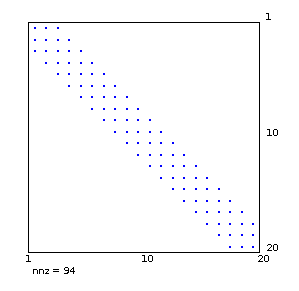
\includegraphics[scale=0.7]{figures/bound.png}
% \label{fig:bound}
% \end{figure}
% 
Nous allons pr\'esenter trois exemples de fonction appartenant \`a la librairie; la fonction bien connue en optimisation Rosenbrock, g\'en\'eralis\'ee \`a dimension variable, 
une fonction trigonom\'etrique et une fonction utilisant les polynômes de Chebychev.
% 
% 
% 
% Comme les polynômes sont de plus en plus compliqu\'es \`a calculer quand la dimension augmente, le coût de $f$
% ne va pas être lin\'eaire par rapport \`a $n$.



\paragraph{Fonction trigonom\'etrique}
\begin{align*}
% \begin{equation}
n \text{ variable, } m=n \\
f_i(x)=n-\sum_{j=1}^{n}cos(x_j)+i(1-cos(x_i))-sin(x_i) \\
x_0= [1/n, \cdots , 1/n] \\
min_x f(x) = 0
% \end{equation}
\end{align*}

% \begin{figure}
% \caption{Matrice hessienne de la fonction trigonom\'etrique}
% \center
% 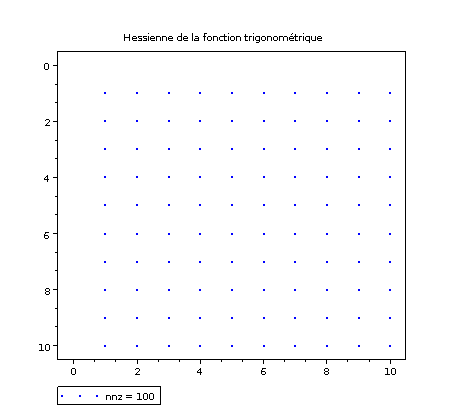
\includegraphics[scale=0.4]{figures/trigo.png}
% \label{fig:trigo}
% \end{figure}


\begin{figure}
\caption{Matrice hessienne de taille 10 par 10 de la fonction trigonom\'etrique, les points bleus repr\'esentent les \'el\'ements non nuls de la
matrice.}

\begin{center}
\fbox{
\begin{minipage}[c]{0.36\textwidth}
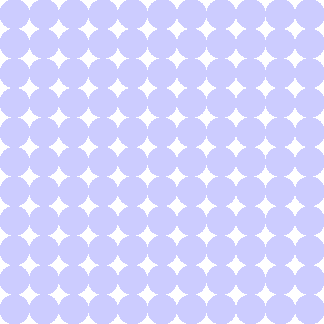
\includegraphics[scale=1]{figures/figure_16}
\end{minipage}
}
\end{center}
\label{fig:trigo}
\end{figure}






La matrice hessienne de la fonction trigonom\'etrique est une matrice pleine \ref{fig:trigo}, cette fonction pourra nous servir 
de r\'ef\'erence car les calculs sont relativement simples.



% \subsection{Fonction Rosenbrock \'etendue}
\paragraph{La fonction Rosenbrock \'etendue}

\begin{align*}
n\text{ variable mais pair } m=2 \\
f_{2i-1}(x)=10(x_{2i}-x^2_{i-1})\\
f_{2i}(x)=1-x_{2i-1}\\
x_0= (\xi_i) \text{ o\`u } \xi_{2i-1}= -1.2  \text{ et } \xi_{2i}=1 \\
min_x f(x) = 0 \text{ en } [1,\cdots ,1]
\end{align*}

Chaque composante de la fonction n'est d\'ependante que de deux variables, c'est pourquoi la matrice hessienne est creuse.

\begin{figure}
\caption{Matrice hessienne de la fonction de Rosenbrock \'etendue}
\begin{center}
\fbox{
\begin{minipage}[c]{0.36\textwidth}
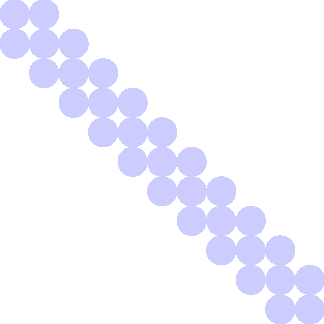
\includegraphics[scale=1]{figures/figure_17}
\end{minipage}
}
\end{center}
\label{fig:rosenbrock}
\end{figure}



% \begin{figure}
% \caption{Newton - La recherche lin\'eaire restreint \`a fournir des it\'er\'es dont la valeur de l'objectif est 
% toujours d\'ecroissante tandis que sans recherche, on s'\'eloigne pour converger plus vite.}
% \begin{center}
% \fbox{
% \begin{minipage}[c]{0.6\textwidth}
% 
% \end{minipage}
% }
% \end{center}
% \label{fig:Newton}
% \end{figure}




La fonction a \'et\'e propos\'ee par Rosenbrock en 1960 afin de comparer des algorithmes de descente. Dans 
le cas avec $n=2$, la fonction forme un sillon \'etroit, ce qui oblige les m\'ethodes de descente \`a suivre une courbe. 
L'agorithme du gradient par exemple est tr\`es m\'ediocre car il "rebondit" sur chaque parois sans avancer vraiment {\co \ref{fig:grarosenbrock}.
La figure de gauche montre les lignes de niveau de la fonction et les droites en bleues correnpondent aux it\'er\'es de l'algorithme du gradient.
L'it\'er\'e initial est \`a gauche et la solution \`a droite. Au milieu, le "saut" a \'et\'e trouv\'e par une recherche lin\'eaire avanc\'ee. La figure de droite
est un zoom de l'algorithme, nous pouvons observer la difficult\'e \`a trouver une direction qui permet d'avancer plus efficacement.}
En ce qui concerne la m\'ethode de Newton, augmenter la dimension de la fonction n'influencera pas le nombre d'it\'erations
car le probl\`eme pourra être vu comme $\frac{n}{2}$ probl\`emes de Rosenbrock qui s'effectuent parall\`element.




\begin{figure}[h]
\caption{Alogrithme du gradient sur Rosenbrock : 19436 it\'erations}
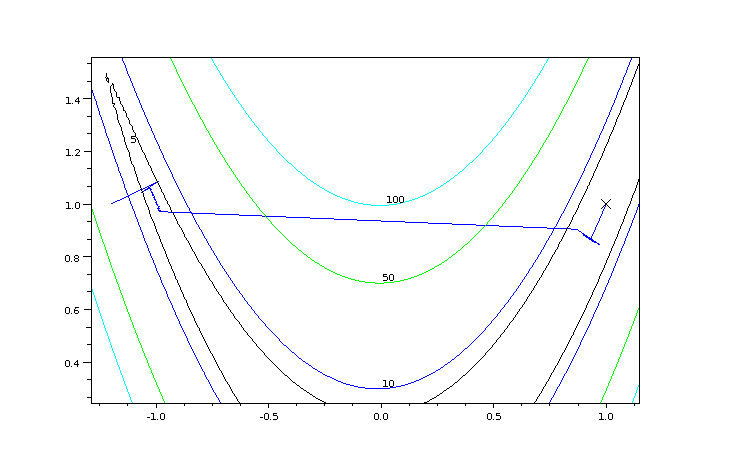
\includegraphics[scale=0.3]{figures/gradient.png}
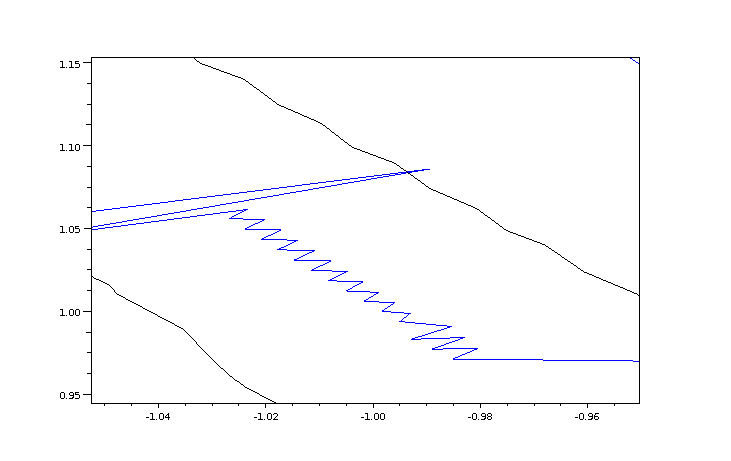
\includegraphics[scale=0.3]{figures/gradientzoom.png}
\label{fig:grarosenbrock}
\end{figure}




% \subsection{Fonction Chebyquad}
\paragraph{La fonction Chebyquad}

\begin{align*}
n \text{ variable, } m=n \\
f_i(x)=\frac{1}{n}\sum_{j=1}^{n}T_i(x_j)-\int_0^1 \! T_i(x)dx \\
\text{O\`u }T_i\text{ est le i\`eme polynôme de Chebychev r\'eduit \`a l'intervale } [0,\ 1] \\
\int_0^1 \! T_i(x)dx= 0 \text{ pour i paire}\\
\int_0^1 \! T_i(x)dx= \frac{-1}{i^2-1} \text{ pour i impaire}\\
x_0= (\xi_j) \text{ o\`u } \xi_j=j/(n+1)\\
f=0 \text{ pour } m=n \text{,}\ 1\leq n\leq 7\ \text{ et }\ n=9\\
f=3.51687... 10^{-3}\ \text{ pour }\ n=m=8 \\
f=6.50395... 10^{-3}\ \text{ pour }\ n=m=10 \\
\end{align*}



% \begin{figure}
% \caption{Matrice hessienne de la fonction de Chebyquad}
% \center
% 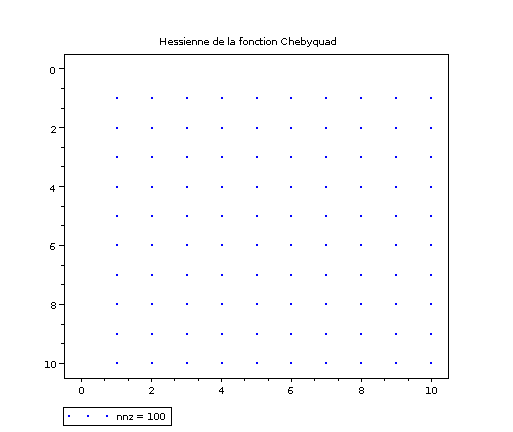
\includegraphics[scale=0.4]{figures/chebyquad.png}
% \label{fig:chebyquad}
% \end{figure}

\begin{figure}
\caption{Matrice hessienne de la fonction de Chebyquad}
\begin{center}
\fbox{
\begin{minipage}[c]{0.36\textwidth}
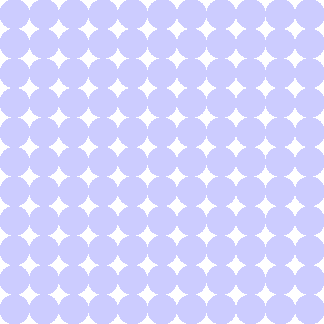
\includegraphics[scale=1]{figures/figure_16}
\end{minipage}
}
\end{center}
\label{fig:chebyquad}
\end{figure}




Ces trois fonctions ont des dimensions variables ; elle refl\`etent l'ensemble des r\'esultats qui sont \'equivalents pour les calculs des d\'eriv\'ees.
La fonction Chebyquad est plus particuli\`ere dans le sens o\`u le temps d'ex\'ecution de la fonction n'est pas proportionnel
\`a la dimension car les polynômes sont de plus en plus complexes \`a calculer en fonction de $n$. 





\paragraph{Temps de calcul du gradient fourni par la routine et du gradient recod\'e}
 Pour la fonction trigonom\'etrique, comme le montre \ref{fig:temps14},
 le calcul du gradient donn\'e par la routine de netlib n'est pas 
efficace. Ceci s'explique par le fait que pour l'obtenir, on utilise la relation $$ \nabla f(x)=F(x)^T\nabla F(x)$$ en notant que 
$$f(x)= \frac{1}{2}\sum_{i=1}^{m}F_i(x)^2$$
Le calcul de la Jacobienne $\nabla F(x)$ de taille $n$ par $m$ impose beaucoup de calculs qui peuvent être \'evit\'es.
En recodant le gradient de la fonction, les multiplications sur les lignes sont factorisables, et en \'evitant le calcul de la 
jacobienne, on am\'eliore nettement l'ex\'ecution. {\co Pour une dimension relativement grande, le temps de calcul du gradient fourni prend plusieurs seconde 
alors que celui de la fonction recod\'e de mani\`ere optimis\'e est instantan\'e.}




\begin{figure}
\caption{Temps d'\'evaluation du gradient en modifiant la taille
de $x$ et celui du gradient recod\'e}
\center
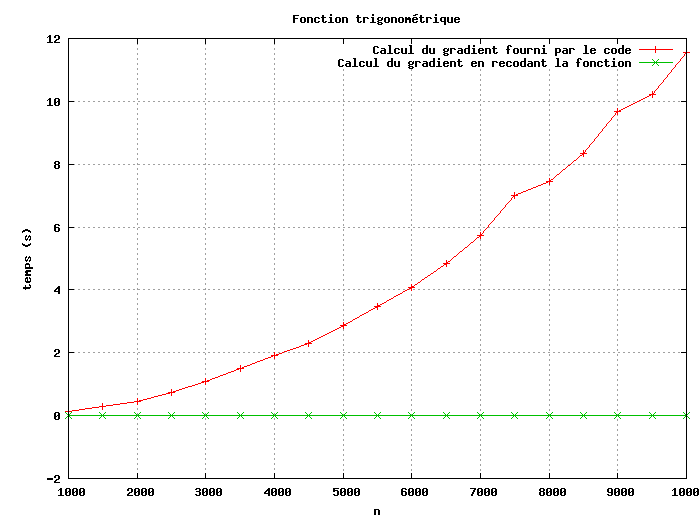
\includegraphics[scale=0.4]{figures/temps14.png}
\label{fig:temps14}
\end{figure}


% \begin{figure}
% \caption{Gradient de la fonction trigonom\'etrique dont le code \`a \'et\'e am\'elior\'e comparativement \`a celui d'origine}
% \center
% 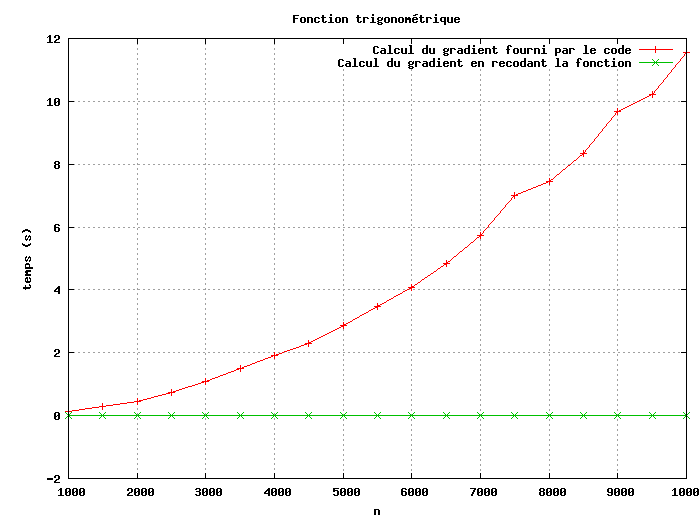
\includegraphics[scale=0.4]{figures/temps14.png}
% \label{fig:temps14}
% \end{figure}




% Avec le code g\'en\'er\'e par tapenade :
% Tableau pour calculer $f(x)$, $\nabla f(x)$,$\nabla^2 f(x)$, $\nabla f(x).v$, $\nabla^2 f(x).uv$



 \paragraph{Comparaison entre l'\'evaluation de la fonction et le mode inverse}

Afin de pouvoir comparer les temps d'ex\'ecution de la fonction et du mode inverse, les appels sont faits
plusieurs fois dans une boucle de mille it\'erations. En effet, même pour une dimension de $n=10000$,
 le temps pour \'evaluer la fonction est inf\'erieur au pas d'horloge unitaire de $4$ms. On remarque sur la
 figure \ref{fig:temps2} que l'obtention du gradient par le mode
inverse est clairement proportionnel au coût de la fonction avec un facteur de proportionnalit\'e d'environ
deux; pour rappel, la borne th\'eorique est de quatre. Le mode inverse est nettement plus performant qu'une implantation na\"ive.


\begin{figure}
\caption{Temps de calcul de la fonction et du gradient en mode direct par {\it Tapenade} dans une boucle de mille it\'erations, fonction trigonom\'etrique}
\center
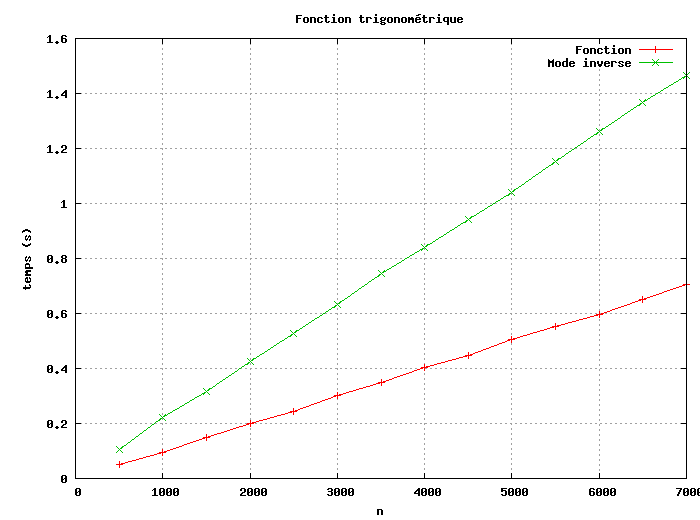
\includegraphics[scale=0.4]{figures/temps2.png}
\label{fig:temps2}
\end{figure}


% La figure \ref{fig:temps6} montre que l'\'evaluation de la fonction Chebyquad n'est pas proportionnelle \`a la dimension; il ne s'agit pas d'une droite.
% En revanche, le gradient ressemble \`a un facteur pr\`es \`a celle de l'\'evaluation. On peut observer que $\#(\nabla f)\simeq 3.5 \#(f)$.
% 
% 
% \begin{figure}
% \caption{Fonction chebyquad, mode inverse vs temps fonction, l'\'evaluation n'est pas proportionnelle \`a la dimension, par contre le gradient 
% ressemble \`a un facteur pr\`es \`a $f$}
% \center
% 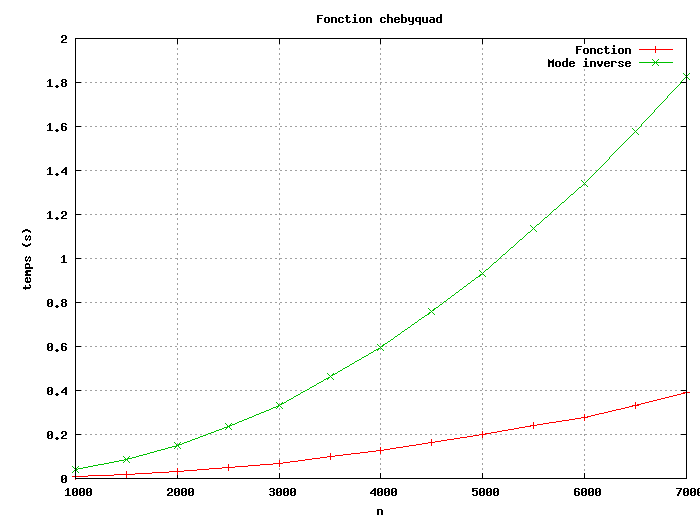
\includegraphics[scale=0.4]{figures/temps6.png}
% \label{fig:temps6}
% \end{figure}



\paragraph{Le mode multi-directionnel}
Le mode multi-directionnel correspond au mode direct appliqu\'e \`a chacune des composantes;
il \'equivaut \`a effectuer $\nabla f(x).(e_i)$ pour chaque $1\leq i\leq n$.
Dans la figure \ref{fig:temps1}, nous pouvons voir que le temps en mode multi-directionnel est
 environ le même que pour calculer le gradient par diff\'erences finies. Le mode multi-directionnel
n'est pas avantageux puisqu'il effectue le mode tangent $n$ fois. {\co La figure \ref{fig:temps4}
permet de comparer le mode multi-directionnel et le mode inverse; pour une dimension assez grande,
le temps de calcul pour le mode multi-directionnel est insatisfaisant et il sera pr\'ef\'erable de l'\'eviter
tant que c'est possible.}

\begin{figure}
\caption{Temps de calcul - fonction trigonom\'etrique}
\center
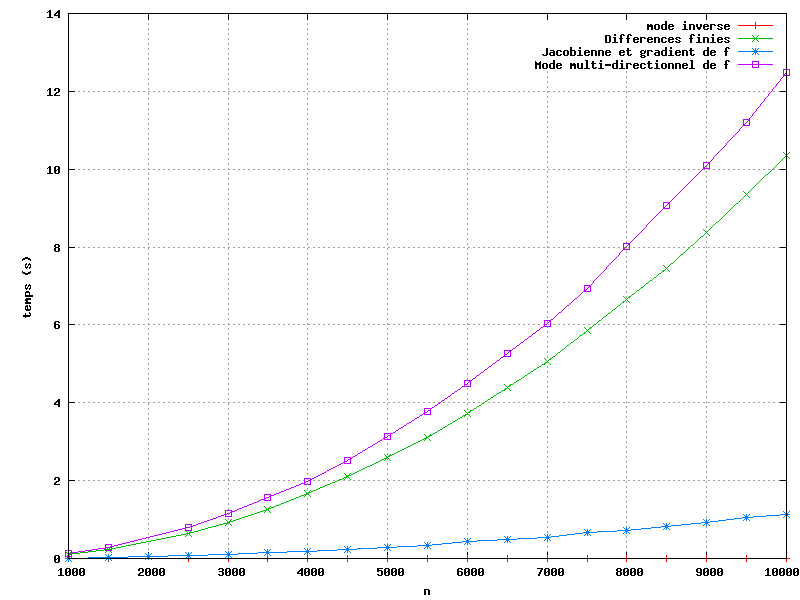
\includegraphics[scale=0.4]{figures/temps1.png}
\label{fig:temps1}
\end{figure}

\begin{figure}
\caption{Mode multi-directionnel : $\nabla f(x)$}
\center
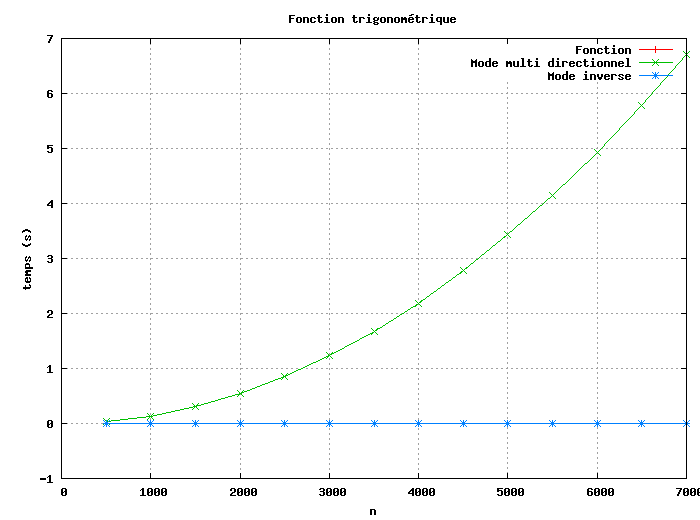
\includegraphics[scale=0.4]{figures/temps4.png}
\label{fig:temps4}
\end{figure}


\paragraph{Hessien$\times$vecteur}

Comme pour le mode inverse, le coût du hessien multipli\'e par un certain vecteur calcul\'e par mode direct sur mode inverse est proportionnel
 au coût de la foncion \ref{fig:temps3} environ 4$\times\#(f)$. {\co En effet, les trois courbes sont tr\`es proches de droites. Ainsi, nous validons
bien que la borne de complexit\'e de $\nabla^2f(x)\cdot v$ est $\mathcal{O}(\#(f))$.}


\begin{figure}
\caption{Mode tangent sur inverse (vert $\times$) sur une boucle de mille it\'erations, ce qui correspond au calcul de $\nabla^2 f(x).v$ pour un certain vecteur, le r\'esultat
est donc aussi un vecteur}
\center
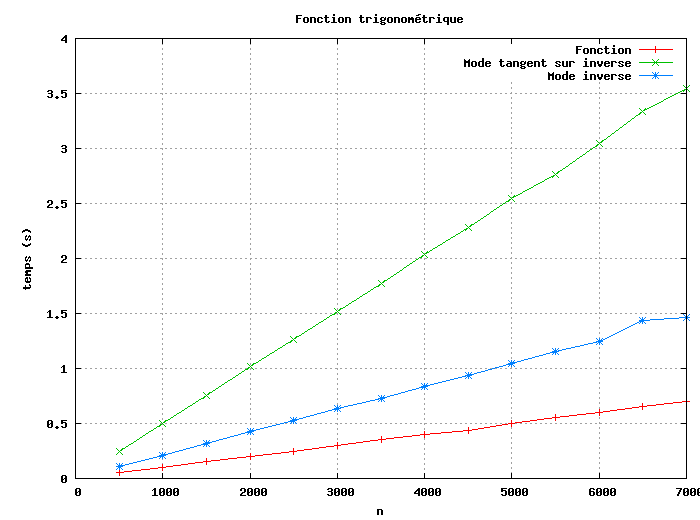
\includegraphics[scale=0.4]{figures/temps3.png}
\label{fig:temps3}
\end{figure}






\paragraph{Hessien}

Pour obtenir la matrice hessienne \ref{fig:temps16}, nous avons pas le choix d'appliquer le mode multi-directionnel. Nous observons cette 
fois ci que le coût est proportionnel \`a $n$ fois le coût de l'\'evaluation de la fonction.


\begin{figure}
\caption{Mode multi-directionnel sur inverse (vert $\times$) ce qui donne la hessienne $\nabla^2 f(x)$ pour un certain vecteur, le r\'esultat
est donc aussi un vecteur}
\center
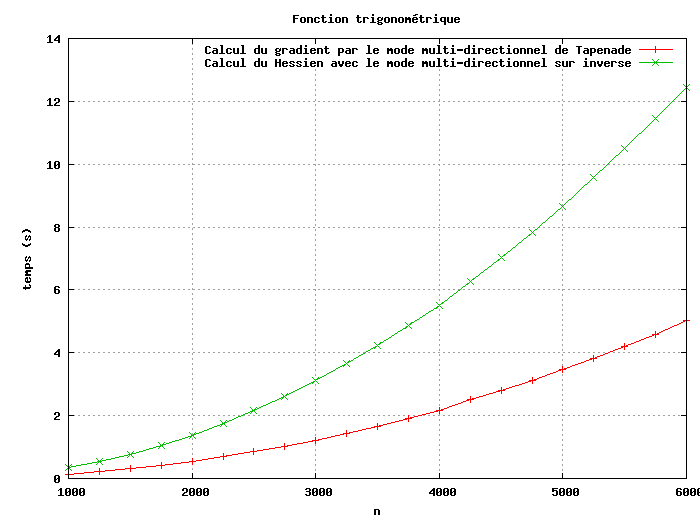
\includegraphics[scale=0.4]{figures/temps16.png}
\label{fig:temps16}
\end{figure}





\paragraph{Ordres sup\'erieurs}
Le coût des op\'erations $\nabla^3 f(x)\cdot u \cdot v$ et $\nabla^4f(x)\cdot u \cdot v \cdot w$ ne d\'ependent pas de $n$ comme le montre la figure
\ref{fig:temps17}. Toutes les courbes sont affines.

\begin{figure}
\caption{Temps des op\'erations  $\nabla^4f(x)\cdot u \cdot v \cdot w$ en vert et marron, $\nabla^3 f(x)\cdot u \cdot v$ en rouge : elles ne d\'ependent pas de $n$
et sont proportionnelles au coût de la fonction.}
\center
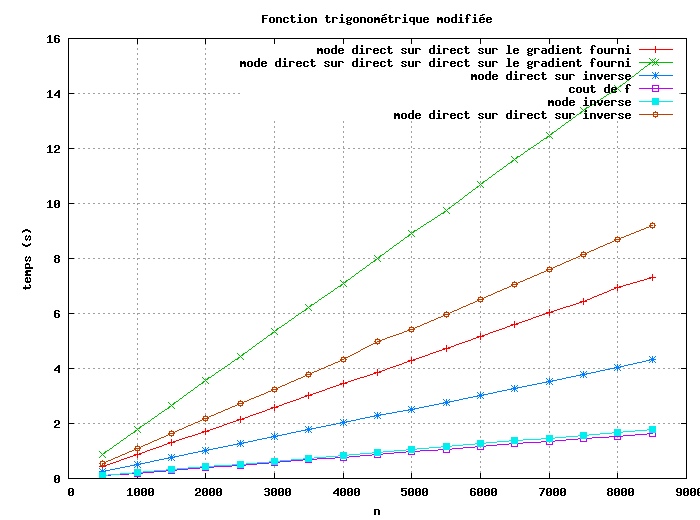
\includegraphics[scale=0.4]{figures/temps17.png}
\label{fig:temps17}
\end{figure}



    \subsection{Avantages et inconv\'enients de {\it Tapenade}}

La transformation du code est la meilleure approche pour la DA; elle donne la capacit\'e de calculer les gradients
\`a un faible coût puisqu'elle ex\'ecute de mani\`ere imp\'erative comme le programme original. De plus, il n'y a pas 
de restriction sur le style ou la taille de l'application \`a diff\'erentier. Au lieu de coder \`a la main une fonction
poss\'edant plusieurs millions de lignes, ce qui est source d'erreurs et demande un effort consid\'erable, il est plus pratique 
de le faire automatiquement. C'est un outil qui progresse encore; les performances du calcul de l'adjoint sont en cours 
d'am\'elioration.
Cependant, il ne traite que du code Fortran et C, même si th\'eoriquement, tous les langages peuvent être trait\'es. Le
sch\'ema optimal de checkpoints imbriqu\'es pour un programme quelconque reste un probl\`eme de recherche.
De plus, les boîtes noires ne peuvent \'evidemment pas être g\'er\'ees, ce qui n'est pas le cas pour la diff\'erentiation par diff\'erences
finies. Pour finir, la plus grosse difficult\'e vient du fait que le logiciel ne g\`ere pas l'ordre trois avec le mode inverse. Il a donc
fallu adapter la librairie mais malgr\'e tout, certains cas ne sont pas fiables, et donne par exemple une hessienne non sym\'etrique.




    \subsection{Difficult\'es pour les d\'eriv\'ees sup\'erieures}

La complexit\'e du stockage des variables lors de la diff\'erentiation automatique est expliqu\'ee dans le livre de Griewank
 \cite{Griewank2008EDP}. Il analyse entre autres le stockage des variables avec l'ordre des op\'erations atomiques et le 
mode inverse r\'ep\'et\'e. Bien qu'efficace, le mode inverse comporte des complications avec {\it Tapenade},
 lorsque l'on veut diff\'erentier \`a un ordre sup\'erieur.
Contrairement au mode tangent qui ne fait que rajouter des op\'erations \'el\'ementaires dans le code, le mode inverse
va faire apparaître des appels \`a des routines : {\tt PUSH} et {\tt POP}. Celles-ci vont permettre de g\'erer une pile qui 
alternativement stockera et restituera les variables tel que d\'ecrit \`a la section \ref{subsection:strategies}. Elles sont cod\'ees en C et appartiennent 
\`a une libraire ext\'erieure mais ne sont pas fournies \`a l'outil de diff\'erentiation. Leur propre code adjoint a \'et\'e cod\'e manuellement
mais seulement \`a l'ordre un par {\it Tapenade}. Pour obtenir des d\'eriv\'ees d'ordre trois, il a fallu coder leurs d\'eriv\'ees.
Lorsque l'on effectue le mode tangent sur tangent sur inverse, certaines routines correspondant aux PUSH et POP ne sont pas correct et il a fallu
les modifier de mani\`ere automatique. Malgr\'e cela, il existe de rares cas o\`u la matrice hessienne n'est pas sym\'etrique mais anti-sym\'etrique. 


{\co 
\section{Conclusion}

Ce chapitre valide les bornes de complexit\'e des calculs pour les d\'eriv\'ees d\'efinies dans le premier chapitre, \`a savoir que 
$\nabla f(x), \nabla^2 f(x)\cdot v$, $\nabla^3 f(x)\cdot v_1\cdot v_2$ et $\nabla^4 f(x)\cdot v_1\cdot v_2\cdot v_3$ ont des coûts 
proportionnels au coût de l'\'evaluation de la fonction. N\'eanmoins, nous avons vu certaines limites de la DA; la difficult\'es de traiter un
code faiblement typ\'e qui accepte certaines astuces et l'obtention des d\'eriv\'ees d'ordre trois et plus avec le mode inverse.
 \`A pr\'esent, comme nous venons d'obtenir ces bornes et que la r\'esolution des
syst\`emes lin\'eaires est efficace nous allons pouvoir comparer les diff\'erentes m\'ethodes de Newton d'ordre sup\'erieur. 
}

%  Pour une d\'ecomposition efficace, j'ai utilis\'e une routine de lapack \cite{lapack}; dsytrf. \\
% Ainsi, pour une matrice sym\'etrique, la d\'ecomposition utilise la m\'ethode de Bunch-Kaufman 
% en pivotant la diagonale\cite{choleskymod}.




 % fichier chapitre-3.tex
% Les choix d'impl\'ementations des op\'erations critiques

%=========================== CHAPITRE 5 ============================
\modeFrancais{}
\chapter[Comparaison des m\'ethodes d'ordres sup\'erieurs] 
        {\singlespacing%
         Comparaison des m\'ethodes de type Newton et d'ordres sup\'erieurs}
         \label{ch:chapitre-5}




\section{Introduction}
Sur l'ensemble des 35 probl\`emes, apr\`es avoir modifi\'e \`a la main les codes g\'en\'er\'es, seuls deux probl\`emes ne donnent
pas une valeur de Hessien correcte par {\it Tapenade}. Nous allons voir dans ce chapitre le temps d'ex\'ecution 
des d\'eriv\'ees et allons v\'erifier que les bornes th\'eoriques de complexit\'e sont respect\'ees. 
Ensuite, nous \'etudierons les variantes de m\'ethodes de descente sur la librairie MGH.


% \section{Temps de calcul des op\'erations critiques}
% Nous allons commencer par \'etudier les op\'erations \'el\'ementaires pour v\'erifier que les m\'ethodes sont comparables.
% Les tests ont \'et\'e effectu\'es sur des fonctions arbitrairement choisies.
% % 




\section{M\'ethode de descente avec recherche lin\'eaire}
Les m\'ethodes d'ordres sup\'erieurs requi\`erent souvent 
moins d'it\'erations. Nous pr\'esentons quelques exp\'eriences illustrant que notre implantation traduit cette r\'eduction du nombre
d'it\'erations dans une r\'eduction du temps de calcul. Les directions ont \'et\'e test\'ees avec et sans recherche lin\'eaire.
Il s'av\`ere que sans recherche lin\'eaire, les algorithmes n'aboutissent pas dans beaucoup de cas car $x_0$ est \'eloign\'e de la solution et
la direction peut être trop grande.
Pour les m\'ethodes de Newton et Chebychev, j'ai d'abord conserv\'e le point initial donn\'e dans les fonctions
de la librairie. Ce point est g\'en\'eralement assez proche de la solution. Dans le tableau, 
nous notons $x_{N_f}$ et $x_{C_f}$ les points finals des m\'ethodes de Newton et Chebychev respectivement. 
Cette norme confirme ou infirme le fait que les deux algorithmes convergent bien vers le même point.

On remarque sur la figure \ref{fig:vraies} que la m\'ethode de Chebychev comme celle d'extrapolation d'ordre trois,
 n'aboutit pas dans plusieurs cas, le maximum d'it\'erations \'etant fix\'e \`a $999$. Afin d'am\'eliorer ceci,
nous allons choisir la direction de Chebychev uniquement lorsqu'il s'agit bien d'une direction de descente.
 Dans le cas contraire nous reprendrons la direction de Newton.

% % Pourquoi n'est pas pertinent ?? On ne sais pas d\'ej\`a que les m\'ethodes convergent tr\`es mal 
% % a priori nous avons pas besoin de direction de descente -> 
% 
% \begin{table}%[h]
% 	\begin{center}
% 
% {\small
% \begin{tabular}{|l|c|c|c|c|c|c|}
%   \hline fonction & n & Iter Newton & Iter Cheb & temps Newton & temps Cheby & $\lVert x_{N_f}-x_{C_f}\rVert $\\
%  \hline
%    rose& $2$ & $22$ & $16$ & $0.020000$ & $0.016000$ & $0.000000$ \\\hline
%    froth& $2$ & $8$ & $6$ & $0.006000$ & $0.005000$ & $0.000000$ \\\hline
%    badscp& $2$ & $999$ & $999$ & $0.871000$ & $6.730000$ & $8.069786$ \\\hline
%    badscb& $2$ & $9$ & $999$ & $0.009000$ & $6.057000$ & $999792.981615$ \\\hline
%    beale& $2$ & $10$ & $999$ & $0.010000$ & $0.889000$ & $1043.480583$ \\\hline
%    jensam& $2$ & $11$ & $8$ & $0.010000$ & $0.007000$ & $0.000000$ \\\hline
%    helix& $3$ & $13$ & $14$ & $0.014000$ & $0.021000$ & $0.000000$ \\\hline
%    bard& $3$ & $13$ & $2$ & $0.013000$ & $0.003000$ & $Nan$ \\\hline
%    gauss& $3$ & $3$ & $3$ & $0.003000$ & $0.003000$ & $0.000000$ \\\hline
%    meyer& $3$ & $163^*$ & $13^*$ & $0.180000$ & $0.041000$ & $1.49\times 10^{10}$ \\\hline
%    gulf& $3$ & $2$ & $2$ & $0.003000$ & $0.027000$ & $Nan$ \\\hline
%    box& $3$ & $20$ & $999$ & $0.020000$ & $4.672000$ & $46.799375$ \\\hline
%    sing& $4$ & $22$ & $15$ & $0.020000$ & $0.013000$ & $0.000032$ \\\hline
%    wood& $4$ & $40$ & $29$ & $0.038000$ & $0.027000$ & $0.000000$ \\\hline
%    kowosb& $4$ & $9$ & $2$ & $0.009000$ & $0.003000$ & $Nan$ \\\hline
%    bd& $4$ & $9$ & $10$ & $0.008000$ & $0.009000$ & $0.000000$ \\\hline
%    rosex& $10$ & $22$ & $999$ & $0.021000$ & $4.290000$ & $2.837129$ \\\hline
%    singx& $12$ & $22$ & $17$ & $0.022000$ & $0.016000$ & $0.000134$ \\\hline
%    pen1& $4$ & $34$ & $999$ & $0.031000$ & $3.441000$ & $0.176609$ \\\hline
%    vardim& $10$ & $15$ & $11$ & $0.015000$ & $0.011000$ & $0.000000$ \\\hline
%    trig& $10$ & $10$ & $999$ & $0.012000$ & $1.080000$ & $2.883\times 10^{48}$ \\\hline
%    almost& $10$ & $9$ & $9$ & $0.008000$ & $0.010000$ & $0.214754$ \\\hline
%    bv& $10$ & $4$ & $3$ & $0.004000$ & $0.003000$ & $0.000000$ \\\hline
%    ie& $10$ & $4$ & $3$ & $0.004000$ & $0.003000$ & $0.000000$ \\\hline
%    band& $10$ & $9$ & $8$ & $0.009000$ & $0.008000$ & $0.000000$ \\\hline
%    cheb& $10$ & $18$ & $999$ & $0.025000$ & $5.302000$ & $0.235547$ \\\hline
%    \end{tabular}
% }
% 	\end{center}
% 	\label{tab:1}
% 	\caption{Tests des m\'ethodes de Newton et Chebychev sur l'ensemble de la librairie MGH avec $x_0$
% relativement proche de la solution. $Nb^*$ signifie que le crit\`ere d'Armijo plante.}
% 	\label{tab:newton}
% \end{table}










\begin{figure}
\caption{Profil des performances sur les fonctions de la librairie MGH, le point initial et les dimensions sont 
ceux par d\'efaut. Les m\'ethodes de Chebychev et Halley n'arrivent pas \`a la solution dans beaucoup de cas.}\center
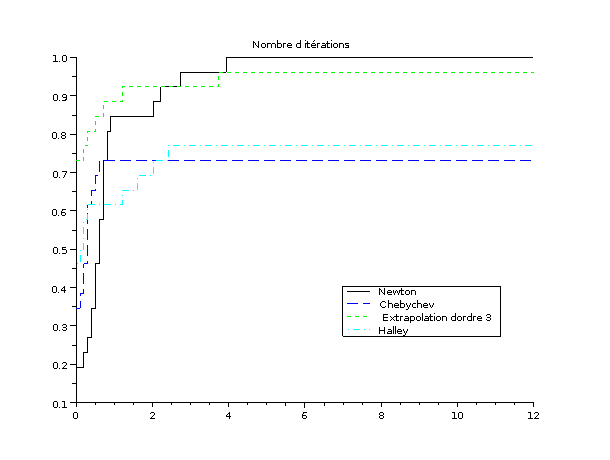
\includegraphics[scale=0.6]{figures/vraiesdirections.png}
\label{fig:vraies}
\end{figure}


L'utilisation de la direction de Newton lorsque celle de Chebychev n'est pas descendante am\'eliore significativement
l'algorithme. En revanche pour Halley, il n'y a presque pas de changement.
\begin{figure}
\caption{Profil des performances : les directions ne sont gard\'ees uniquement s'il s'agit de direction de descente, sinon on 
reprend celle de Newton. Cette fois-ci l'extrapolation d'ordre trois r\'eussit pour tous les probl\`emes.
}\center
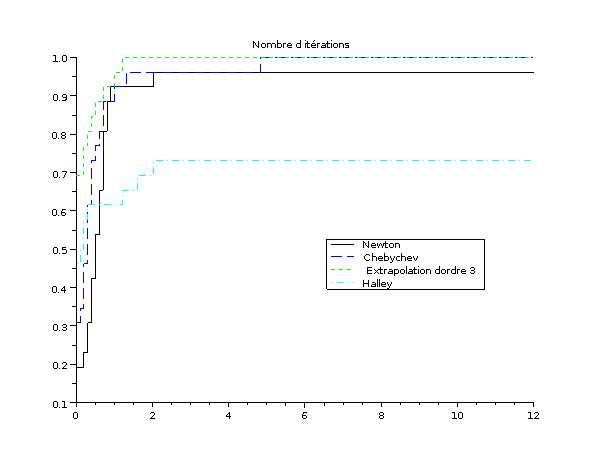
\includegraphics[scale=0.6]{figures/newtonquandpasdescendante.png}
\label{fig:dirnewton}
\end{figure}





% \begin{table}[h]
% 	\begin{center}
% {%\small
%  \footnotesize
% % ---------------------------------------sans l'extrapolation d'ordre 3
% % \begin{tabular}{|l|c|c|c|c|c|c|}
% %   \hline fonction & n & Iter Newton & Iter Cheb & temps Newton & temps Cheby &$\lVert x_{N_f}-x_{C_f}\rVert $\\
% %  \hline
% %    rose& $2$ & $22$ & $16$ & $0.020000$ & $0.017000$ & $0.000000$ \\\hline
% %    froth& $2$ & $8$ & $6$ & $0.007000$ & $0.005000$ & $0.000000$ \\\hline
% %    badscp& $2$ & $999$ & $545$ & $0.878000$ & $0.475000$ & $0.082534$ \\\hline
% %    badscb& $2$ & $9$ & $21$ & $0.009000$ & $0.037000$ & $0.000000$ \\\hline
% %    beale& $2$ & $10$ & $9$ & $0.011000$ & $0.011000$ & $0.000000$ \\\hline
% %    jensam& $2$ & $11$ & $8$ & $0.010000$ & $0.007000$ & $0.000000$ \\\hline
% %    helix& $3$ & $13$ & $14$ & $0.014000$ & $0.022000$ & $0.000000$ \\\hline
% %    bard& $3$ & $13$ & $13$ & $0.013000$ & $0.014000$ & $0.000000$ \\\hline
% %    gauss& $3$ & $3$ & $3$ & $0.003000$ & $0.003000$ & $0.000000$ \\\hline
% %    meyer& $3$ & $163^*$ & $133^*$ & $0.181000$ & $0.177000$ & $0.000000$ \\\hline
% %    gulf& $3$ & $2$ & $2$ & $0.003000$ & $0.004000$ & $Nan$ \\\hline
% %    box& $3$ & $20$ & $135$ & $0.020000$ & $0.132000$ & $66.947050$ \\\hline
% %    sing& $4$ & $22$ & $15$ & $0.020000$ & $0.013000$ & $0.000032$ \\\hline
% %    wood& $4$ & $40$ & $29$ & $0.038000$ & $0.027000$ & $0.000000$ \\\hline
% %    kowosb& $4$ & $9$ & $9$ & $0.009000$ & $0.009000$ & $0.000000$ \\\hline
% %    bd& $4$ & $9$ & $10$ & $0.009000$ & $0.009000$ & $0.000000$ \\\hline
% %    rosex& $10$ & $22$ & $20$ & $0.022000$ & $0.025000$ & $0.000000$ \\\hline
% %    singx& $12$ & $22$ & $17$ & $0.022000$ & $0.017000$ & $0.000134$ \\\hline
% %    pen1& $4$ & $34$ & $25$ & $0.031000$ & $0.023000$ & $0.000000$ \\\hline
% %    vardim& $10$ & $15$ & $11$ & $0.014000$ & $0.010000$ & $0.000000$ \\\hline
% %    trig& $10$ & $10$ & $9$ & $0.012000$ & $0.012000$ & $0.000000$ \\\hline
% %    almost& $10$ & $9$ & $9$ & $0.008000$ & $0.009000$ & $0.214754$ \\\hline
% %    bv& $10$ & $4$ & $3$ & $0.004000$ & $0.003000$ & $0.000000$ \\\hline
% %    ie& $10$ & $4$ & $3$ & $0.004000$ & $0.003000$ & $0.000000$ \\\hline
% %    band& $10$ & $9$ & $8$ & $0.009000$ & $0.008000$ & $0.000000$ \\\hline
% %    cheb& $10$ & $18$ & $20$ & $0.026000$ & $0.031000$ & $0.103538$ \\\hline
% %    \end{tabular}
% 
% \begin{tabular}{|l|c|c|c|c|c|c|c|c|c|}
%   \hline fonction & n & IN & IC & I3 & T N & T C& T E3 &  $\lVert x_{N_f}-x_{C_f}\rVert $ & $\lVert x_{N_f}-x_{3_f}\rVert $ \\
%  \hline
%    rose& $2$ & $22$ & $16$ & $15$ & $0.020$& $0.016$ & $0.019$  & $0.000000$ & $0.000000$ \\\hline
%    froth& $2$ & $8$ & $6$ & $5$ & $0.006$& $0.005$ & $0.005$  & $0.000000$ & $0.000000$ \\\hline
%    badscp& $2$ & $999$ & $545$ & $288$ & $0.874$& $0.477$ & $0.312$ & $0.082534$ & $0.235713$ \\\hline
%    badscb& $2$ & $9$ & $21$ & $18$ & $0.009$& $0.036$ & $0.075$ & $0.000000$ & $0.000000$ \\\hline
%    beale& $2$ & $10$ & $9$ & $8$ & $0.010$& $0.011$ & $0.020$ & $0.000000$ & $0.000000$ \\\hline
%    jensam& $2$ & $11$ & $8$ & $7$ & $0.009$& $0.007$ & $0.008$ & $0.000000$ & $0.000000$ \\\hline
%    helix& $3$ & $13$ & $14$ & $11$ & $0.013$& $0.022$ & $0.017$ & $0.000000$ & $0.000000$ \\\hline
%    bard& $3$ & $13$ & $13$ & $13$ & $0.013$& $0.014$ & $0.017$ & $0.000000$ & $0.000000$ \\\hline
%    gauss& $3$ & $3$ & $3$ & $3$ & $0.002$& $0.002$ & $0.003$ & $0.000000$ & $0.000000$ \\\hline
%    meyer& $3$ & $163^*$ & $133^*$ & $146^*$ & $0.196$& $0.184$ & $0.376$ & $0.000000$ & $0.000000$ \\\hline
%    gulf& $3$ & $2$ & $2$ & $2$ & $0.003$& $0.003$ & $0.010$ & $Nan$ & $Nan$ \\\hline
%    box& $3$ & $20$ & $135$ & $11$ & $0.020$& $0.131$ & $0.017$ & $66.947050$ & $0.000000$ \\\hline
%    sing& $4$ & $22$ & $15$ & $13$ & $0.020$& $0.014$ & $0.014$ & $0.000032$ & $0.000068$ \\\hline
%    wood& $4$ & $40$ & $29$ & $25$ & $0.038$& $0.027$ & $0.030$ & $0.000000$ & $0.000000$ \\\hline
%    kowosb& $4$ & $9$ & $9$ & $9$ & $0.010$& $0.009$ & $0.012$ & $0.000000$ & $0.000000$ \\\hline
%    bd& $4$ & $9$ & $10$ & $11$ & $0.008$& $0.009$ & $0.013$ & $0.000000$ & $0.000000$ \\\hline
%    rosex& $10$ & $22$ & $20$ & $13$ & $0.021$& $0.024$ & $0.023$ & $0.000000$ & $0.000000$ \\\hline
%    singx& $12$ & $22$ & $17$ & $16$ & $0.022$& $0.017$ & $0.020$ & $0.000134$ & $0.000155$ \\\hline
%    pen1& $4$ & $34$ & $25$ & $19$ & $0.031$& $0.023$ & $0.021$ & $0.000000$ & $0.000000$ \\\hline
%    vardim& $10$ & $15$ & $11$ & $10$ & $0.015$& $0.011$ & $0.012$ & $0.000000$ & $0.000000$ \\\hline
%    trig& $10$ & $10$ & $9$ & $9$ & $0.012$& $0.011$ & $0.017$ & $0.000000$ & $0.000000$ \\\hline
%    almost& $10$ & $9$ & $9$ & $12$ & $0.008$& $0.009$ & $0.020$ & $0.214754$ & $0.000000$ \\\hline
%    bv& $10$ & $4$ & $3$ & $3$ & $0.004$& $0.003$ & $0.004$ & $0.000000$ & $0.000000$ \\\hline
%    ie& $10$ & $4$ & $3$ & $3$ & $0.004$& $0.003$ & $0.003$ & $0.000000$ & $0.000000$ \\\hline
%    band& $10$ & $9$ & $8$ & $7$ & $0.009$& $0.008$ & $0.010$ & $0.000000$ & $0.000000$ \\\hline
%    cheb& $10$ & $18$ & $20$ & $13$ & $0.025$& $0.031$ & $0.039$ & $0.103538$ & $0.323658$ \\\hline
% 
% 
%    \end{tabular}
% }
% 	\end{center}
% 	\caption{Tests des m\'ethodes de Newton et Pseudo-Chebychev sur l'ensemble de la librairie MGH avec $x_0$
% relativement proche de la solution : pour Chebychev et l'extrapolation d'ordre 3 la direction n'est gard\'ee que s'il s'agit d'une 
% direction descendante sinon on reprend celle de Newton.}
% 	\label{tab:newton}
% \end{table}


Ensuite, j'ai effectu\'e les mêmes tests mais avec des dimensions plus grandes. Comme point de d\'epart,
j'ai d'abord choisi un nombre donn\'e par la fonction random, \`a valeurs comprises entre z\'ero et cent. Sachant que les algorithmes ne sont pas 
globalement convergents, le tableau \ref{tab:111} montre ce fait et en g\'en\'eral, ils ne convergent pas vers le même point.
Pour le tableau \ref{tab:dimplus}, j'ai choisi $1$, $10$ ou $100$ fois la valeur du point initial de la librairie MGH. Dans les cas o\`u 
les m\'ethodes convergent vers le même point, on peut noter une am\'elioration dans le nombre d'it\'erations. {\co
Pour la premi\`ere fonction du tableau, la diff\'erence des normes n'est pas \'egale mais les points finals obtenus ont un gradient v\'erifiant la condition
$\nabla f(x) \leq \epsilon$. L'\'ecart entre la valeur de l'objectif entre ces points est tr\`es faible. }
 En ce qui concerne le temps d'ex\'ecution,
il est meilleur pour Chebychev mais pour l'extrapolation d'ordre trois les temps sont moins bon car j'ai du partir du code fourni par le code des fonctions
car il n'est pas possible d'atteindre l'ordre $4$ avec Tapenade, même en essayant de modifier les routines PUSH et POP.
 



% \begin{table}%[h]
% 	\begin{center}
% {\small
% \begin{tabular}{|l|c|c|c|c|c|c|}
%   \hline fonction & $n$ & Iter Newton & Iter Cheb & temps Newton & temps Cheby & $\lVert x_{N_f}-x_{C_f}\rVert $ \\
%  \hline
% trig& $100 $&$ 6$ &$ 6 $&$ 0.072000 $&$ 0.056000 $&$ 0.000000$ \\\hline %en utilisant le x0
% ie& $300 $&$ 4 $&$ 3 $&$ 1.842000 $& $1.395000 $&$ 0.000000 $\\\hline % en utilisant le x0
% ie& $500 $&$ 4 $& $3 $& $8.047000$ &$ 6.110000 $&$ 0.000000$ \\\hline % en utilisant le x0
% ie& $800 $&$ 4 $& $3 $& $32.200000 $& $24.464000 $&$ 0.000000$ \\\hline % en utilisant le x0
% ie& $300 $&$ 7 $& $5 $& $3.204000$ & $2.324000$ & $0.000000$ \\\hline   % en utilisant le 10* x0
% ie& $500 $&$ 7 $& $5 $& $14.045000 $& $10.163000$ & $0.000000$ \\\hline % en utilisant le 10* x0
% ie& $800 $&$ 7 $&$ 5 $& $56.345000 $& $40.795000 $& $0.000000$ \\\hline % en utilisant le 10* x0
% band& $300$ &$ 9 $& $8$ &$ 0.352000 $& $0.345000 $& $0.000000 $\\\hline  % en utilisant le x0
% band& $500$ &$ 9 $& $8 $& $0.923000 $& $0.884000 $& $0.000000 $\\\hline  % en utilisant le x0
% band& $800$ &$ 9 $& $8 $& $2.566000 $& $2.450000 $& $0.000000 $\\\hline  % en utilisant le x0
% band& $300$ &$ 19$ & $15$ &$ 0.718000$ &$ 0.629000 $& $0.000000$ \\\hline
% \end{tabular}
% }
% 	\end{center}
% 	\caption{Point initial proche suffisamment proche de la solution pour que Chebychev converge : le gain en it\'eration
% n'est pas tr\`es grand. En revanche si la dimension est grande, le gain en temps peut être bon.}
% 	\label{tab:der}
% \end{table}

\begin{table}%[h]
	\begin{center}
{\small
\begin{tabular}{|l|c|c|c|c|c|c|c|c|c|c|}
  \hline fonction & $k*x_0$ & $n$ & IN & IC & I3 & TN & TC & T3 & $\lVert x_{N_f}-x_{C_f}\rVert $ & $\lVert x_{N_f}-x_{3_f}\rVert $  \\
 \hline
bv & 1 & 300 & 2 & 2 & 2 & 0.043 & 0.043 & 0.074 & 0.000042 & 0.000042 \\\hline 
bv & 10 & 300 & 4 & {\bf 3} & 4 & 0.082 & 0.065 & 0.149 & 0.000228 & 0.000308 \\\hline 
bv & 100 & 300 & 13 & {\bf 10 }& 11 & 0.266 & 0.218 & 0.413 & 0.000029 & 0.000267 \\\hline 
bv & 1 & 500 & 7 & 6 & {\bf 4} & 0.407 & 0.375 & 0.433 & 0.000725 & 0.000473 \\\hline 
bv & 10 & 500 & 13 & 13 & 15 & 0.747 & 0.815 & 1.626 & 0.001876 & 0.002417 \\\hline 
bv & 100 & 500 & 23 &{\bf 19} & 21 & 1.323 & 1.193 & 2.289 & 0.001084 & 0.000554 \\\hline 
bv & 1 & 800 & 6 & 5 &{\bf 3} & 1.062 & 0.942 & 0.920 & 0.016409 & 0.141987 \\\hline 
bv & 10 & 800 & 11 & 9 & {\bf 7} & 1.938 & 1.717 & 2.175 & 0.706669 & 0.924390 \\\hline 
bv & 100 & 800 & 21 &{\bf 20} & 17 & 3.720 & 3.841 & 5.325 & 0.798127 & 0.800345 \\\hline
ie & 1 & 300 & 4 & 3 & 3 & 1.834 & 1.398 & 1.468 & 0.000 & 0.000000 \\\hline 
ie & 10 & 300 & 7 & 5 & 5 & 3.205 & 2.330 & 2.474 & 0.000 & 0.000000 \\\hline 
ie & 1 & 500 & 4 & 3 & 3 & 8.044 & 6.105 & 6.348 & 0.000 & 0.000000 \\\hline 
ie & 10 & 500 & 7 & 5 & 5 & 14.054 & 10.155 & 10.556 & 0.000 & 0.000000 \\\hline 
ie & 1 & 800 & 4 & 3 & 3 & 32.521 & 24.463 & 25.169 & 0.000 & 0.000000 \\\hline 
ie & 10 & 800 & 7 & 5 & 5 & 56.313 & 40.456 & 41.555 & 0.000 & 0.000000 \\\hline 
trid & 1 & 300 & 7 & 6 & 6 & 0.152 & 0.129 & 0.204 & 0.000 & 0.000000 \\\hline 
trid & 10 & 300 & 12 & 10 & 10 & 0.246 & 0.215 & 0.344 & 0.000 & 0.000000 \\\hline 
trid & 100 & 300 & 18 & 15 & 14 & 0.369 & 0.325 & 0.482 & 0.000 & 0.000000 \\\hline 
trid & 1 & 500 & 7 & 6 & 6 & 0.397 & 0.366 & 0.579 & 0.000 & 0.000000 \\\hline 
trid & 10 & 500 & 12 & 10 & 10 & 0.673 & 0.613 & 0.967 & 0.000 & 0.000000 \\\hline 
trid & 100 & 500 & 18 & 15 &{\bf 14} & 1.015 & 0.906 & 1.333 & 0.000 & 0.000000 \\\hline 
trid & 1 & 800 & 7 & 6 & 6 & 1.177 & 1.080 & 1.656 & 0.000 & 0.000000 \\\hline 
trid & 10 & 800 & 12 & 10 & 10 & 2.043 & 1.842 & 2.757 & 0.000 & 0.000000 \\\hline 
trid & 100 & 800 & 18 & 15 & 14 & 3.067 & 2.760 & 3.854 & 0.000 & 0.000000 \\\hline 
band & 1 & 300 & 9 & 8 &{\bf 7} & 0.330 & 0.321 & 0.416 & 0.000 & 0.000000 \\\hline 
band & 10 & 300 & 19 & 15 & 15 & 0.695 & 0.608 & 0.894 & 0.000 & 0.000000 \\\hline 
band & 100 & 300 & 29 & 23 & 23 & 1.061 & 0.933 & 1.372 & 0.000 & 0.000000 \\\hline 
band & 1 & 500 & 9 & 8 &{\bf 7} & 0.904 & 0.895 & 1.149 & 0.000 & 0.000000 \\\hline 
band & 10 & 500 & 19 & 15 & 15 & 1.894 & 1.633 & 2.398 & 0.000 & 0.000000 \\\hline 
band & 100 & 500 & 29 & 23 & 23 & 2.892 & 2.508 & 3.680 & 0.000 & 0.000000 \\\hline 
band & 1 & 800 & 9 & 8 &{\bf 7} & 2.538 & 2.408 & 3.018 & 0.000 & 0.000000 \\\hline 
band & 10 & 800 & 19 & 15 & 15 & 5.391 & 4.570 & 6.468 & 0.000 & 0.000000 \\\hline 
band & 100 & 800 & 29 & 23 & 23 & 8.231 & 7.040 & 9.933 & 0.000 & 0.000000 \\\hline 
\end{tabular}
}
	\end{center}
	\caption{En testant avec des dimensions plus grandes. Comme point initial : 1, 10 ou 100 fois $x_0$. Le temps pour 
l'extrapolation d'odre 3 est plus grand car les d\'eriv\'ees sont calcul\'ees \`a partir du gradient fourni et non du mode inverse.
Les points finals de la premi\`ere fonction v\'erifient les conditions d'un gradient suffisamment petit.}
\label{tab:dimplus}


\end{table}

% \subsection{Avec r\'egion de confiance}
\subsection{Figures qui illustrent les parcours}


\paragraph{Rosenbrock}

Sur les figures \ref{fig:Newton} et \ref{fig:Chebychev}, j'ai trac\'e le chemin qu'emprunte 
l'algorithme de Newton et de Chebychev pour la fonction de Rosenbrock.
On observe bien que sans recherche lin\'eaire, l'algorithme est plus rapide,
cependant la valeur de l'objectif peut augmenter. \`A l'it\'eration $2$, la valeur de l'objectif
 atteint $1411.8$, et si l'algorithme revient vers la solution, c'est {$\scriptscriptstyle\ll$}par chance{$\scriptscriptstyle\gg$} car il n'y a pas de convergence globale.
 Lorsque l'on applique une recherche lin\'eaire, le parcours est mieux contrôl\'e et suit une {$\scriptscriptstyle\ll$}vall\'ee{$\scriptscriptstyle\gg$} o\`u la valeur de la
fonction objectif reste faible.

\begin{figure}
\caption{Newton - La recherche lin\'eaire restreint \`a fournir des it\'er\'es dont la valeur de l'objectif est 
toujours d\'ecroissante tandis que sans recherche, on s'\'eloigne pour converger plus vite.}
\begin{center}
\fbox{
\begin{minipage}[c]{0.6\textwidth}
\beginpgfgraphicnamed{figures/courbe_0}
\endpgfgraphicnamed \\
	  \begin{tabular}{|l|c|c|c|}
	  \hline
	  it\'eration & $x_1$ & $x_2$ &  $f(x)$ \\
	  \hline
	  $0$ & $-1.200000$ & $1.000000$ & $24.200000$ \\
	  $1$ & $-1.175281$ & $1.380674$ & $4.731884$ \\
	  $2$ & $0.763115$ & $-3.175034$ & $1411.845179$ \\
	  $3$ & $0.763430$ & $0.582825$ & $0.055966$ \\
	  $4$ & $0.999995$ & $0.944027$ & $0.313189$ \\
	  $5$ & $0.999996$ & $0.999991$ & $0.000000$ \\
	  $6$ & $1.000000$ & $1.000000$ & $0.000000$ \\
	  \hline
	  \end{tabular}\\
\end{minipage}
}
\end{center}
\label{fig:Newton}
\end{figure}

% \vspace{1cm}


% \begin{table}%[h]
% 	\begin{center}
% 	  \begin{tabular}{|l|c|c|c|}
% 	  \hline
% 	  it\'eration & $x_1$ & $x_2$ &  $f(x)$ \\
% 	  \hline
% 	  $0$ & $-1.200000$ & $1.000000$ & $24.200000$ \\
% 	  $1$ & $-1.175281$ & $1.380674$ & $4.731884$ \\
% 	  $2$ & $0.763115$ & $-3.175034$ & $1411.845179$ \\
% 	  $3$ & $0.763430$ & $0.582825$ & $0.055966$ \\
% 	  $4$ & $0.999995$ & $0.944027$ & $0.313189$ \\
% 	  $5$ & $0.999996$ & $0.999991$ & $0.000000$ \\
% 	  $6$ & $1.000000$ & $1.000000$ & $0.000000$ \\
% 	  \hline
% 	  \end{tabular}\\
% 	\end{center}
% 	\caption{It\'er\'es de la m\'ethode de Newton sur la fonction Rosenbrock sans recherche lin\'eaire.}
% 	\label{tab:newton}
% \end{table}





\begin{figure}
\caption{Chebychev - La direction de Chebychev est meilleure sur l'exemple, cependant qu'une seule it\'eration n'est gagn\'ee}
\begin{center}
\fbox{
\begin{minipage}[c]{0.6\textwidth}
% \begin{center}
\beginpgfgraphicnamed{figures/courbe_1}
\endpgfgraphicnamed \\
	\begin{tabular}{|l|c|c|c|}
	\hline
	it\'eration & $x_1$ & $x_2$ &  $f(x)$ \\
	\hline
	$0$ & $-1.200000$ & $1.000000$ & $24.200000$ \\
	$1$ & $-1.150840$ & $1.322626$ & $4.626437$ \\
	$2$ & $0.848588$ & $-0.780668$ & $225.254139$ \\
	$3$ & $0.849592$ & $0.721806$ & $0.022623$ \\
	$4$ & $1.000000$ & $0.999993$ & $0.000000$ \\
	$5$ & $1.000000$ & $1.000000$ & $0.000000$ \\
	\hline
	\end{tabular}
%\end{center}
\end{minipage}
}
\end{center}
% \beginpgfgraphicnamed{figures/courbe_1}
% \endpgfgraphicnamed

\label{fig:Chebychev}
\end{figure}


% \begin{table}%[h]
% 	\begin{center}
% 	\begin{tabular}{|l|c|c|c|}
% 	\hline
% 	it\'eration & $x_1$ & $x_2$ &  $f(x)$ \\
% 	\hline
% 	$0$ & $-1.200000$ & $1.000000$ & $24.200000$ \\
% 	$1$ & $-1.150840$ & $1.322626$ & $4.626437$ \\
% 	$2$ & $0.848588$ & $-0.780668$ & $225.254139$ \\
% 	$3$ & $0.849592$ & $0.721806$ & $0.022623$ \\
% 	$4$ & $1.000000$ & $0.999993$ & $0.000000$ \\
% 	$5$ & $1.000000$ & $1.000000$ & $0.000000$ \\
% 	\hline
% 	\end{tabular}
% 	\end{center}
% 	\caption{It\'er\'es de la m\'ethode de Chebychev sur la fonction Rosenbrock}
% 	\label{tab:chebychev}
% \end{table}




\begin{figure}%[!h]
\caption{Ordre sup\'erieur : la direction s'\'eloigne encore moins de la vall\'ee que les proc\'ed\'es de Newton ou Chebychev.}
\begin{center}
\fbox{
\begin{minipage}[c]{0.7\textwidth}
\beginpgfgraphicnamed{figures/courbe_2}
\endpgfgraphicnamed \\
	\begin{tabular}{|l|c|c|c|}
	\hline
	it\'eration & $x_1$ & $x_2$ &  $f(x)$ \\
	\hline
	$0$ & $-1.200000$ & $1.000000$ & $24.200000$ \\
	$1$ & $-1.126673$ & $1.265834$ & $4.524003$ \\
	$2$ & $0.847210$ & $-0.350714$ & $114.187943$ \\
	$3$ & $0.849335$ & $0.721366$ & $0.022700$ \\
	$4$ & $1.000000$ & $1.000000$ & $0.000000$ \\
	$5$ & $1.000000$ & $1.000000$ & $0.000000$ \\
	\hline
	\end{tabular}\\
\end{minipage}
}
\end{center}
\label{fig:sup}
\end{figure}





% \begin{table}%[!h]
% 	\begin{center}
% 	\begin{tabular}{|l|c|c|c|}
% 	\hline
% 	it\'eration & $x_1$ & $x_2$ &  $f(x)$ \\
% 	\hline
% 	$0$ & $-1.200000$ & $1.000000$ & $24.200000$ \\
% 	$1$ & $-1.126673$ & $1.265834$ & $4.524003$ \\
% 	$2$ & $0.847210$ & $-0.350714$ & $114.187943$ \\
% 	$3$ & $0.849335$ & $0.721366$ & $0.022700$ \\
% 	$4$ & $1.000000$ & $1.000000$ & $0.000000$ \\
% 	$5$ & $1.000000$ & $1.000000$ & $0.000000$ \\
% 	\hline
% 	\end{tabular}\\
% 	\end{center}
% 	\caption{It\'er\'es de la m\'ethode d'extrapolation d'ordre 3 sur la fonction Rosenbrock}
% 	\label{tab:extra3}
% \end{table}


% \cite{historical}\cite{cauchy}

{\co
\section{Conclusion}
Par l'interpr\'etation de ces r\'esultats, nous pouvons conclure qu'il est possible d'obtenir des m\'ethodes convergant plus rapidement
que la m\'ethode de Newton dans un cas g\'en\'eral. De plus, l'efficacit\'e est meilleure; les temps de calcul sont r\'eduits. Malheureusement,
la DA est encore immature pour fournir l'ordre 4 de mani\`ere efficace. On peut cependant esp\'erer que les outils de DA seront bientôt capable
d'atteindre ces ordres de d\'erivations de mani\`ere syst\'ematique. En ce sens, nous pourrons gagner du temps grâce au m\'ethodes d'ordre sup\'erieur
et ce, d'autant que la dimension du probl\`eme est grande.
}
 % fichier chapitre-4.tex

\modeFrancais{}
% \include{contenu_maitrise/conclusion}
\Conclusion

Nous avons r\'eussi \`a d\'evelopper un environnement au sein de {\it Scilab}, grâce \`a une interface avec 
fortran, nous permettant d'obtenir les d\'eriv\'ees d'ordres sup\'erieurs de la librairie de Mor\'e, Garbow, Hilstrom.
Le logiciel Tapenade a \'et\'e adapt\'e pour fournir ces d\'eriv\'ees de mani\`ere efficace, y compris l'ordre trois alors 
qu'il n'est pas conçu pour le faire en mode inverse.
D'autre part, la g\'en\'ericit\'e des fonctions de la librairie de MGH a permis une automatisation de la g\'en\'eration des codes 
diff\'erenti\'es. \'Etant donn\'e que ces fonctions ont toutes les mêmes arguments, la diff\'erentiation se fait toujours par rapport 
aux mêmes variables. Ainsi, pour automatiser le traitement et la g\'en\'eration des codes diff\'erenti\'es, il suffit
d'avoir des fonctions ayant les mêmes param\`etres.
Enfin, grâce \`a cet environnement nous avons impl\'ement\'e des m\'ethodes efficaces notamment avec 
une d\'ecomposition de Cholesky modifi\'ee
provenant de la librairie {\it Fortran} LAPACK pour la r\'esolution des syst\`emes lin\'eaires.
Ainsi, plusieurs m\'ethodes ont pu être test\'ees, parfois sold\'ees par des directions non pertinentes, parfois par des
directions meilleures que les classiques de Newton et Chebychev.
Cependant, la g\'en\'eration du code demande un pr\'e-traitement du code source lorsqu'il n'est pas \'ecrit de mani\`ere rigoureuse
 ou trop astucieuse. De plus, comme Tapenade n'a pas \'et\'e conçu pour utiliser le mode inverse \`a un ordre sup\'erieur \`a deux,
des incoh\'erences apparaissent \`a l'ordre trois avec ce mode et il faut modifier le code que Tapenade produit. Le r\'esultat n'est pas fiable 
\`a cent pourcent. Par cons\'equent, ces parties de code \`a modifier ne peuvent pas être automatis\'ees. Voir l'annexe \ref{annexe:C} pour plus de d\'etails.
 Même si le gain en temps n'est pas 
\'enorme, on peut esp\'erer que les versions futures de Tapenade pour les ordres trois et quatre permettront cette avanc\'ee.

Il est certain que les progr\`es de la DA vont ouvrir la voie \`a des m\'ethodes d'optimisation plus \'elabor\'ees. Comme nous l'avons
vu, la complexit\'e est d'utiliser la tranformation de code pour l'efficacit\'e. En effet, la surcharge des op\'erateurs 
est beaucoup plus flexible et facile \`a utiliser mais plus lente. La transformation de code requiert des calculs 
explicites et sans astuces. 
{\co 
 Une fois cette \'etape franchie, nous pourrions voir apparaître des m\'ethodes plus 
performantes remplaçant la m\'ethode de Newton. En r\'ealit\'e, ce genre de m\'ethodes ne seraient qu'applicables sur 
des probl\`emes o\`u la m\'ethode de Newton marche, sinon il y a de fortes chances pour que ces m\'ethodes \'echouent aussi. 
N\'eanmoins, dans ce cas, pour des dimensions relativement grandes, elles pourraient permettre un gain de temps.

On peut imaginer qu'\`a l'avenir, certains compilateurs pourraient int\'egrer des outils de DA permettant d'obtenir des ordres sup\'erieurs sans
l'intervention humaine, c'est-\`a-dire que le proc\'ed\'e serait enti\`erement automatis\'e. En effet, en analysant le code source du programme principal,
il serait en mesure de savoir quel ordre \`a atteindre et quels param\`etres utiliser.

}
\nocite{choleskymod}
\nocite{355936}
\nocite{Iri89onautomatic}
% \nocite{autodiff} ,
% \nocite{librairie},
% \nocite{tapenade}, 
% \nocite{lapack}, 
\nocite{convnewton}
\nocite{diffautoopa}
\nocite{Griewank2008EDP}
\nocite{paresseuse} 
\nocite{differentiaauto}
\nocite{historical}
\nocite{cauchy}
\nocite{implementation}
\nocite{Kantorovich}
\nocite{Higham}
\nocite{Baur}
\nocite{Ulbrich}
\nocite{Kchouk}
\nocite{Bunch}
\nocite{More}
\nocite{Corliss1991b}
\nocite{opt}
\nocite{nocedal99}

%%=================================================================
%%========================== ANNEXES ==============================
%%=================================================================

\appendix
\renewcommand{\chaptermark}[1]{\markboth{\textsc{\appendixname\ \thechapter.\ #1}}{}}
%% Les annexes peuvent \^etre en fran\c{c}ais ou en anglais
%% Si elles sont en anglais, elles doivent contenir \modeAnglais ou \englishMode
%% juste apr\`es la commande \chapter{xxx}

%%=========================== ANNEXE A ============================

\modeFrancais{}
\chapter{Premi\`ere annexe}
\label{annexe:A}


\section{D\'efinitions}
\label{annexe:A:def}

\begin{frdefinition}\textbf {(Fonction continue)} \\
Soient $f:X\subseteq\mathbb{R}^n\rightarrow\mathbb{R}^m$ et $x_0\in X$. La fonction f est continue en $x_0$ 
si et seulement si
 $$\lim_{x\rightarrow x_0} f(x)=f(x_0)$$
c'est-\`a-dire que si, pour tout $\epsilon \in \mathbb{R}$, $\epsilon>0$, il existe $\eta>0$ tel que 
$$\lVert x-x_0\rVert < \eta \text{ et } x \in X \Rightarrow \lVert f(x)-f(x_0)\rVert < \epsilon$$
\end{frdefinition}


\begin{frdefinition}\textbf {(Valeurs et vecteurs propres)} \\
Soit une matrice carr\'ee $M\in \mathbb{R}^{n\times n}$. Les valeurs propres de $A$ sont les racines 
de son polyn\^ome caract\'eristique
$$p_M(z)=\det(zI-M)$$
o\`u $I$ est la matrice identit\'e de dimension $n$. Si $\lambda$ est une valeur propre de $A$, les vecteurs
$x\in \mathbb{R}^n$ non nuls tels que $$ Mx=\lambda x$$
sont appel\'es vecteurs propres.
\end{frdefinition}


\begin{frdefinition}\textbf {(Matrice d\'efinie positive)} \\
Une matrice carr\'ee $A \in \mathbb{R}^{n\times n}$ est dite d\'efinie lorsque \\
$$x^TAx>0, \ \forall x\in \mathbb{R}^n, \ x\neq 0$$
si de plus $A$ est sym\'etrique, toutes ses valeurs propres sont strictement positives. 
\end{frdefinition}



\begin{frdefinition}\textbf {(Matrice bande)} \\
Une matrice carr\'ee $A \in \mathbb{R}^{n\times n}$ est dite matrice bande si tout ses \'el\'ements 
en dehors de la bande diagonale born\'ee par deux constantes $k_1$ et $k_2$ sont nuls:
\begin{equation*}
 a_{ij}=0 \text{  si  }  j < i-k_1 \text{  ou  } j >i+k_2, \ k_1,k_2 \geq 0 
\end{equation*}



\end{frdefinition}





\begin{frdefinition}\textbf {(Fonction lipschitzienne)} \\
Soit $I$ un intervalle de $\mathbb{R}$ non vide et non r\'eduit \`a un point et 
$f:I\rightarrow \mathbb{R}$ une application alors on dit que f est 
$k$-lipschitzienne s'il existe un $k$ r\'eel strictement positif tel que
\begin{equation}
 \forall (x,y)\in I^2, |f(x)-f(y)|\leq k|x-y|
\end{equation}
La constante k est dite constante de Lipschitz.
\end{frdefinition}


 % fichier annexe-A.tex

%%=========================== ANNEXE B ============================

\modeFrancais{}



\chapter{Les difficult\'es rencontr\'ees}
\label{annexe:C}

\section{Librairie Mor\'e, Garbow et Hillstrom}


Sur le site de netlib\footnote{\url{http://www.netlib.org}}, on peut retrouver plusieurs librairies \'ecrites en fortran.
Celle qui nous int\'eresse se trouve plus pr\'ecis\'ement dans les probl\`emes sans contraintes\footnote{\url{http://www.netlib.org/uncon/data/}}.


Pour faciliter l'utilisation de tapenade, les fichiers sources ont dû être modifi\'es.
Tout d'abord, j'ai nomm\'e les fonctions par leur nom (\`a la place de {\tt getfun}) pour pouvoir avoir un appel
unique \`a la routine. J'ai remplac\'e tous les appels \`a la fonction {\tt ddot} par les op\'erations 
qu'effectue cette routine (produit scalaire). 
Il arrive qu'au lieu de passer un vecteur en argument, on donne un scalaire : {\tt g(j) = ddot( m, fj( 1, j), 1, f, 1)} l.155
 dans rose.f par exemple, ce qui a pour effet de multiplier la $j$\`eme colonne de {\tt fj} par {\tt f}. Cependant, Tapenade ne peut analyser
ce code pour le diff\'erentier parce qu'il s'agit d'une astuce sur l'incr\'ementation de {\tt fj(1,j)} qui donne {\tt fj(2,j)} ce qui est 
propre au fonctionnement interne de Fortran.




De plus, certains param\`etres ne sont initialis\'es que pour le mode $-1$ lors de l'appel \`a la fonction or 
ces param\`etres sont utilis\'es pour les autres modes. J'ai donc rajout\'e cette initialisation au d\'ebut de 
la fonction. Par exemple {\tt nqrtr  = 1} au d\'ebut sing.f.





\begin{itemize}
\item Changement du nom des routines getfun par le nom de la fonction (celui du fichier)
\item Remplacement des ddot par la somme des carr\'es
\item Remplacement des dcopy par copie \'el\'ements par \'el\'ements
\item Rajout des initialisations des param\`etres qui le sont uniquement dans le mode $-1$
\item parameter (one = 1.d0) n'est pas d\'efini dans badscp.f !! 
\item Rajout de {\tt ftf=0d0} pour \'eviter d'additionner les valeurs lorsque l'on fait plusieurs appels
\end{itemize}

L'ensemble de ces modifications peut être retrouv\'e dans le script {\tt make}.





\section{M\'ethodes d'ordres sup\'erieurs}

Comme le montre le tableau suivant, le point initial a une grande importance dans l'ex\'ecution des m\'ethodes. 
En choisissant un point al\'eatoire, il y a moins de chance pour que les algorithmes convergent vers le même point. D'autre part,
la convergence n'est pas garantie.

\begin{table}%[h]
	\begin{center}
{\small
%%%%%%%%%%%%%%%%%%%%%%%%%%%%%%%%%%%%%% Si la m\'ethode de Chebychev n'est pas une direction de Descente 
%on la garde quand meme!!!!!!!!!!!!!!!!!!!!!!!!!!!!!!!!!!!!!!!!!!!
\begin{tabular}{|l|c|c|c|c|c|c|}
  \hline fonction & $n$ & Iter Newton & Iter Cheb & temps Newton & temps Cheby & Norme diff \\
 \hline
   rose& 2 & 77 & 5 & 0.075 & 0.004 & 0.000000 \\\hline
   froth& 2 & 17 & 12 & 0.015 & 0.011 & 0.000000 \\\hline
   badscp& 2 & $19^*$ & 999 & 0.104 & 5.140 & 73081.313391 \\\hline
   badscb& 2 & 18 & 999 & 0.024 & 5.814 & 999915.027828 \\\hline
   beale& 2 & $14^*$ & 999 & 0.074 & 4.536 & 28470.397921 \\\hline
   jensam& 2 & 1 & 1 & 0.001 & 0.002 & Nan \\\hline
   helix& 3 & 14 & 10 & 0.013 & 0.014 & 0.000000 \\\hline
   bard& 3 & 9 & 2 & 0.009 & 0.002 & Nan \\\hline
   gauss& 3 & 1 & 1 & 0.001 & 0.001 & 0.000000 \\\hline
   meyer& 3 & $271^*$ & 999 & 0.302 & 6.159 & 6168.587560 \\\hline
   gulf& 3 & 1 & 1 & 0.001 & 0.001 & 0.000000 \\\hline
   box& 3 & 21 & 6 & 0.021 & 0.016 & Nan \\\hline
   sing& 4 & 26 & 19 & 0.024 & 0.017 & 0.000136 \\\hline
   wood& 4 & 27 & 21 & 0.025 & 0.024 & 0.000000 \\\hline
   kowosb& 4 & 230 & 2 & 0.221 & 0.003 & Nan \\\hline
   bd& 4 & 13 & 12 & 0.013 & 0.011 & 0.000000 \\\hline
   rosex& 10 & 203 & 5 & 0.207 & 0.005 & 0.000000 \\\hline
   singx& 12 & 30 & 24 & 0.030 & 0.023 & 0.000553 \\\hline
   pen1& 4 & 42 & 30 & 0.038 & 0.027 & 0.000000 \\\hline
   vardim& 10 & 26 & 19 & 0.025 & 0.018 & 0.000000 \\\hline
   trig& 10 & 20 & 2 & 0.023 & 0.027 & Nan \\\hline
   almost& 10 & 25 & 28 & 0.078 & 0.297 & Nan \\\hline
   bv& 10 & 22 & 999 & 0.022 & 5.438 & 185.331743 \\\hline
   ie& 10 & 21 & 17 & 0.025 & 0.029 & 0.000000 \\\hline
   band& 10 & 31 & 25 & 0.033 & 0.034 & 0.000000 \\\hline
   cheb& 10 & 167 & 999 & 0.208 & 5.010 & 1.674059 \\\hline
   ie & 100 & 89 & 360 & 2.251 & 11.208 & 0.000000 \\\hline 
   ie& 200 & 177 & 234 & 27.493 & 39.950 & 0.000000 \\\hline
   trig& 100 & 46 & 45 & 0.340 & 0.343 & 0.069866 \\\hline 
   trig& 250 & 61 & 58 & 2.104 & 2.114 & 14217.789748 \\\hline  
   trig& 350 & 61 & 65 & 4.270 & 4.700 & 0.022663 \\\hline  
   bv& 500 & 20 & 16 & 1.172 & 1.016 & 0.0066708 \\\hline
   bv& 1 & 19 & 15 & 5.404 & 4.585 &  0.1489379 \\\hline
   bv& 1500 & 17 & 14 & 10.86 & 9.613 & 12.905217 \\\hline
   bv& 2 & 17 & 13 & 19.097 & 15.863 & 17.806732 \\\hline
\end{tabular}
}
	\end{center}
	\caption{Nombre d'it\'eration des m\'ethodes de Newton et Chebychev mais sur un point initial loin de la 
solution. Les algorithmes convergent rarement au même point.}
	\label{tab:111}
\end{table}
 % fichier annexe-B.tex

%%=========================== ANNEXE C ============================

\modeFrancais{}
\chapter{Troisi\`eme annexe}
\label{annexe:C}

\section{La surcharge des op\'erateurs}

\paragraph{Programmation paresseuse}

Pour commencer \`a me familiariser avec la diff\'erentiation automatique, j'ai d'abord essay\'e de 
concevoir un programme qui d\'erive en programmation fonctionnelle. D'apr\`es l'article de Karczmarczuk \cite{paresseuse}, il est possible 
de calculer la diff\'erentiation automatique avec un langage fonctionnel de mani\`ere paresseuse.
La s\'emantique du programme original va être \'etendue par surcharge des op\'erateurs en utilisant
les r\`egles usuelles de d\'erivation. Par exemple, la r\`egle de Leibniz $(fg)'=f'g+fg'$ o\`u la r\`egle
d'encha\^inement : $(f(g(x))'=f'(g(x))g(x)$. Pour toutes op\'erations \'el\'ementaires, nous allons surcharger
par les op\'erations de d\'erivation. Pour cela, on consid\`ere une paire $(e,e')$ qui repr\'esente la valeur
orginale et sa d\'eriv\'ee. De cette mani\`ere, les constantes seront repr\'esent\'ees par $(c,0)$ et la variable
$(x,1)$. Toutes les op\'erations vont être surcharg\'ees pour ce type : $(f,f')+(g,g')=(f+g,f'+g')$, 
$(f,f')\cdot(g,g')=(f\cdot g,f'\cdot g+f\cdot g')$, $cos(f,f')=(cos(f),cos(f)\cdot f')$ et ainsi de suite.

Le langage fonctionnel que j'ai choisi est caml. On commence par d\'efinir un type expression qui traduit les op\'erations \'el\'ementaires. Comme il
 s'agit d'un exemple, la liste est non exhaustive. Le type expression est d'abord introduit, il va nous permettre d'analyser le type d'op\'eration.
En caml, il est impossible de faire un "match" sur une fonction par exemple : \begin{verbatim}| cos -> sin \end{verbatim}
c'est pour cette raison que l'on d\'efinit un constructeur de type : expression. 
{\small
\begin{verbatim}
type expression= 
    Const of float
  | Var of string
  | Opp of expression
  | Plus of expression*expression
  | Moins of expression*expression
  | Mult of expression*expression
  | Quot of expression*expression
  | Puiss of expression*float
  | Cos of expression
  | Sin of expression
  | Exp of expression
  | Log of expression
;;
\end{verbatim}
}
\noindent
Pour diff\'erentier nos constantes de nos variables, il faut introduire lors de l'\'evaluation un
environnement qui fournira la valeur de chaque variable. Par exemple si $x=3.5$ et $y=-2.1$,
$env=[("x",3.5);("y",-2.1)]$ (les parenth\`eses ne sont pas n\'ecessaires mais permettent de bien
comprendre qu'il s'agit d'une liste de couples).


Ainsi, pour \'evaluer une expression, nous n'aurons plus qu'\`a faire :

\begin{verbatim}
let rec evaluer env expr = match expr with
    Const c-> c 
  | Var v->(try List.assoc v env with Not_found ->
 raise(Unbound_variable v))
  | Opp f-> -.evaluer env f
  | Plus(f,g) -> evaluer env f +. evaluer env g
  | Moins(f,g) -> evaluer env f -. evaluer env g
  | Mult(f,g) -> evaluer env f *. evaluer env g
  | Quot(f,g) -> evaluer env f /. evaluer env g
  | Puiss(f,g) ->(evaluer env f)**g
  | Cos(f) -> cos(evaluer env f)
  | Sin(f) -> sin(evaluer env f)
  | Log(f) -> log (evaluer env f)
  | Exp(f) ->  exp (evaluer env f)
 ;;
\end{verbatim}
\noindent
{\tt List.assoc v env} permet de renvoyer l'\'el\'ement correspondant \`a {\tt v} dans la liste de couple {\tt env}. Avec notre exemple,
{\tt List.assoc "x" env} retourne {\tt 3.5}. Cette \'evaluation est la traduction du GAO. Le point apr\`es l'op\'erateur signifie que les composantes sont des {\it float}. (Les op\'erateurs
ne sont pas surcharg\'es et le \verb!+! est pour les entiers).


Pour \'evaluer la d\'eriv\'ee: 

{\small
\begin{verbatim}
let rec derive expr dv =
    match expr with
      Const c -> Const 0.0
    | Var v -> if v = dv then Const 1.0 else Const 0.0
    | Opp f -> Opp(derive f dv)
    | Plus(f, g) -> Plus(derive f dv, derive g dv)
    | Moins(f, g) -> Moins(derive f dv, derive g dv)
    | Mult(f, g) -> Plus(Mult(f, derive g dv), Mult(derive f dv, g))
    | Quot(f, g) -> Quot(Moins(Mult(derive f dv, g), Mult(f, derive g dv)),
                         Mult(g, g))
    | Puiss(f,g) -> Mult(Const g,Mult(derive f dv,f))
    | Cos(f) -> Opp(Mult(Sin(f),derive f dv))
    | Sin(f) -> Mult(Cos(f),derive f dv)
    | Exp(f) -> Mult(derive f dv,Exp(f))
    | Log(f) -> Quot(derive f dv,f)
 ;;
\end{verbatim}
}
\noindent
Karczmarczuk a propos\'e une mani\`ere d'obtenir les d\'eriv\'ees d'ordres sup\'erieurs de mani\`ere paresseuse avec Haskell,
un langage fonctionnel. La d\'efinition pr\'ec\'edente est reprise et \'etendue mais sur une liste infinie $f::f'::f''::f^{(3)}\cdots $
repr\'esentant l'expression avec l'ensemble de ses d\'eriv\'ees. 
De la même mani\`ere, les constantes seront repr\'esent\'ees par $c::0::0\cdots$
et la variable $x::1::0::0\cdots$. En notant $f=(f_0::\bar f)$ et $g=(g_0::\bar g)$ o\`u $f_0$, $g_0$ sont
les \'el\'ements en tête de liste et $\bar f$, $\bar g$ sont les listes queues, les op\'erations seront d\'efinies :
$$f+g = (f_0+g_0::\bar f+\bar g)$$
$$f\cdot g = (f_0\cdot g_0::f\cdot \bar g+\bar f\cdot g)$$
$$f/g = w \text{  o\`u  }(f_0/g_0::(\bar f\cdot g+f \cdot\bar g)\cdot w^2)$$


\noindent
On observe que la d\'efinition est auto-r\'ecursive. \'Evidemment, nous ne devrons pas \'evaluer toute la liste mais seulement les 
d\'eriv\'ees qui nous int\'eressent. Si on essaye d'obtenir {\tt w}, on boucle \`a l'infini! 
\'Etant donn\'e que {\it Caml}\footnote{{\url http://caml.inria.fr/}} n'est pas un langage paresseux, contrairement \`a Haskell, il a fallu construire un nouveau type que l'on 
\'evaluera uniquement quand nous en aurons besoin.


{\small
\begin{verbatim}
type 'a glacon =
| Inconnu of (unit -> 'a)
| Connu of ' a;;
\end{verbatim}
}
\noindent
Le type \verb!(unit -> 'a)! repr\'esente une fonction sans argument. Le r\'esutlat n'est que potentiellement pr\'esent; uniquement 
lorsque l'on \'evaluera cette fonction.

{\small
\begin{verbatim}
type 'a liste_paresseuse =
| Nil
| Cons of 'a cellule
and 'a cellule = { hd : 'a; mutable tl : 'a liste_paresseuse glacon};;
\end{verbatim}
}


{\small
\begin{verbatim}
let force cellule =
  let glacon = cellule.tl in
  match glacon with
  | Connu valeur -> valeur
  | Inconnu g ->
     let valeur = g () in
     cellule.tl <- Connu valeur;
     valeur;;
\end{verbatim}
}
\noindent
Forcer la cellule revient \`a \'evaluer la fonction \verb!g!.
\begin{figure}
\caption{Temps d'\'evaluation du gradient en mode direct par surcharge des op\'erateurs sur 
des listes et vecteurs avec caml}
\begin{center}
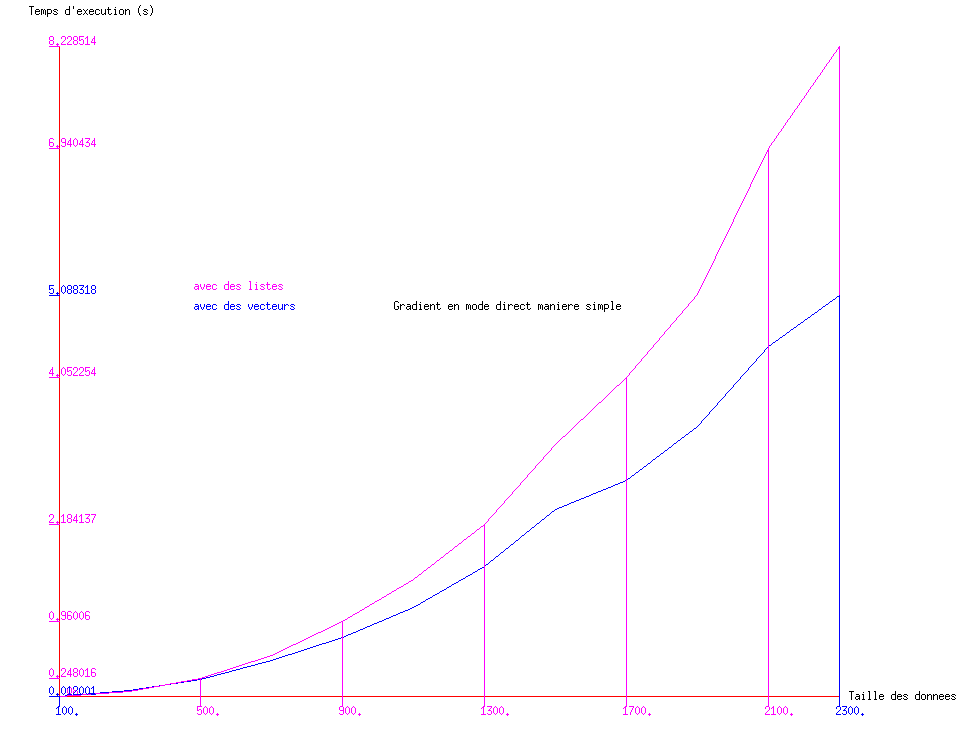
\includegraphics[scale=0.6]{figures/caml1.png}
\end{center}
\label{fig:caml1}
\end{figure}
La figure \ref{fig:caml1} illustre le fait que ces op\'erations impliquent des structures de plus en plus complexes \`a g\'erer.




On peut g\'en\'eraliser les listes infinies \`a plusieurs dimensions avec des d\'eriv\'ees partielles :
$f=(f_0,[\bar f_1,\cdots, \bar f_n] $ o\`u $\bar f_k=(\partial f/\partial f_k,[\cdots \text{ d\'eriv\'ees de }f_k' \cdots])$.
L'inconv\'enient d'une telle m\'ethode vient de la structure qui est rapidement lourde \`a g\'erer; les listes sont tr\`es dures
\`a manipuler lorsqu'elles sont de grandes tailles; $\mathcal{O}(n)$ dans le pire des cas et les vecteurs ne sont pas dynamiques.\\


 % fichier annexe-C.tex

%=================================================================
%=================== BIBLIOGRAPHIE ET INDEX ======================
%=================================================================

% --- Bibliographie
\bibliographystyle{style/frplainUDS}
% le contenu est dans un fichier bibliographie.bib. 
% Il est possible de mettre plusieurs noms de fichiers s\'epar\'es par une virgule.
\bibliography{bibliographie}  
% --- Bibliographie

\end{document}













